\documentclass[12pt,a4paper]{article}

%------------------------------------------------
% PAQUETES
%------------------------------------------------
\usepackage[utf8]{inputenc}
\usepackage[T1]{fontenc}
\usepackage[spanish,es-tabla]{babel}
\usepackage{geometry}
\geometry{margin=2.5cm}

\usepackage{setspace}
\onehalfspacing

\usepackage{graphicx}
\usepackage{float}
\usepackage{booktabs}
\usepackage{caption}
\usepackage{amsmath,amssymb,amsfonts}
\usepackage{xcolor}
\usepackage{listings}
\usepackage{fancyhdr}
\usepackage{hyperref}

%------------------------------------------------
% ESTILO PARA EL CÓDIGO PYTHON
%------------------------------------------------
\definecolor{codegreen}{rgb}{0,0.45,0}
\definecolor{codegray}{rgb}{0.45,0.45,0.45}
\definecolor{codepurple}{rgb}{0.55,0,0.75}
\definecolor{backcolour}{rgb}{0.96,0.96,0.93}

\lstdefinestyle{mystyle}{
    backgroundcolor=\color{backcolour},
    commentstyle=\color{codegreen},
    keywordstyle=\color{magenta},
    numberstyle=\tiny\color{codegray},
    stringstyle=\color{codepurple},
    basicstyle=\ttfamily\footnotesize,
    breaklines=true,
    captionpos=b,
    keepspaces=true,
    numbers=left,
    numbersep=5pt,
    showspaces=false,
    showstringspaces=false,
    showtabs=false,
    tabsize=4,
    % permite tildes dentro del código
    literate={á}{{\'a}}1 {é}{{\'e}}1 {í}{{\'i}}1 {ó}{{\'o}}1 {ú}{{\'u}}1 {ñ}{{\~n}}1
}
\lstset{style=mystyle}

%------------------------------------------------
% ENCABEZADOS
%------------------------------------------------
\pagestyle{fancy}
\fancyhf{}
\fancyhead[L]{Cálculo Aplicado}
\fancyhead[R]{Integración numérica}
\fancyfoot[C]{\thepage}

\hypersetup{
colorlinks=true,
linkcolor=blue,
urlcolor=blue
}

%------------------------------------------------
\begin{document}

%%%%%%%%%%%%%%%%%%%%%%%%%%%%%%%%%%%%%%%%%%%%%%%%%%
% PORTADA
%%%%%%%%%%%%%%%%%%%%%%%%%%%%%%%%%%%%%%%%%%%%%%%%%%

\begin{titlepage}
\thispagestyle{empty}

\begin{center}

\vspace*{1.5cm}

%-------------------------------------------------
% Logo de la UCU
% Subir el archivo "logo.png" al proyecto de Overleaf
%-------------------------------------------------
% \includegraphics[width=10cm]{logo.png}

\vspace{1.8cm}

{\Huge\textbf{Comparación de Métodos de Integración Numérica}}

\vspace{0.6cm}

{\Large Proyecto grupal}

\vspace{2cm}

\renewcommand{\arraystretch}{1.6}

\begin{tabular}{rl}
\textbf{Asignatura:} & Cálculo Aplicado \\
\textbf{Estudiantes:} & Mikaela Dominguez \\
                      & Juliana Hernandez \\
                
\textbf{Docente:} & Renzo Ferradini\\
\textbf{Fecha:} & \today \\
\end{tabular}

\vfill

{\large Universidad Católica del Uruguay}
\vspace{0.3cm}

{\Large Campus Punta del Este}

\end{center}

\end{titlepage}

%%%%%%%%%%%%%%%%%%%%%%%%%%%%%%%%%%%%%%%%%%%%%%%%%%
% NUMERACIÓN ROMANA
%%%%%%%%%%%%%%%%%%%%%%%%%%%%%%%%%%%%%%%%%%%%%%%%%%

\pagenumbering{roman}

\section*{Resumen}

En este trabajo aproximamos numéricamente la integral \(\int_{-1}^{1}2\sqrt{1-x^2}\,dx=\pi\) con distintos métodos de integración numérica implementados en Python. En el Ejercicio 1 calculamos las sumas inferior y superior con particiones equiespaciadas y comprobamos que ambas convergen a \(\pi\), lo que confirma que la función es integrable de Riemann. En el Ejercicio 2 comparamos tres formas de construir la partición (equiespaciada, aleatoria uniforme y cosenoidal) y encontramos que la cosenoidal da el menor error en todos los casos, porque concentra los puntos cerca de los extremos, donde la curva es más empinada. En el Ejercicio 3 comparamos los métodos de rectángulos, trapecio y punto medio sobre una misma partición equiespaciada: el punto medio fue el más preciso, rectángulos y trapecio coincidieron porque la función vale cero en los extremos, y tanto el trapecio como el punto medio convergieron mucho más rápido que las sumas de Darboux.
\clearpage

\tableofcontents

\clearpage

%%%%%%%%%%%%%%%%%%%%%%%%%%%%%%%%%%%%%%%%%%%%%%%%%%
% NUMERACIÓN ARÁBIGA
%%%%%%%%%%%%%%%%%%%%%%%%%%%%%%%%%%%%%%%%%%%%%%%%%%

\pagenumbering{arabic}

%=====================================================================
% informe.tex  —  SOLO CONTENIDO (sin \documentclass ni \begin{document})
% Se incluye desde main.tex con %=====================================================================
% informe.tex  —  SOLO CONTENIDO (sin \documentclass ni \begin{document})
% Se incluye desde main.tex con %=====================================================================
% informe.tex  —  SOLO CONTENIDO (sin \documentclass ni \begin{document})
% Se incluye desde main.tex con \input{informe}
%=====================================================================

% Los bloques de código se llaman "Código 1, 2, 3" en lugar de "Listing"
\renewcommand{\lstlistingname}{Código}

%=====================================================================
\section{Ejercicio 1: Convergencia de las sumas inferior y superior}
%=====================================================================

\subsection{Introducción y análisis teórico}

La función y el intervalo bajo estudio son:
\[
f(x)=2\sqrt{1-x^2}, \qquad x\in[-1,1].
\]

La ecuación \(x^2+y^2=1\) describe el círculo unitario. Su semicircunferencia superior corresponde a \(y=\sqrt{1-x^2}\). La función del ejercicio es el doble de dicha altura, es decir, \(f(x)=2y\). El área de la semicircunferencia unitaria es \(\pi/2\); al duplicar las alturas, el área exacta bajo la curva es:
\[
\int_{-1}^{1}2\sqrt{1-x^2}\,dx=\pi.
\]

\subsection{Cómo se forman las sumas}

Para un valor de \(N\), se consideran \(N\) puntos equiespaciados, que generan \(N-1\) subintervalos de igual ancho:
\[
\Delta x=\frac{1-(-1)}{N-1}=\frac{2}{N-1}.
\]
Los puntos de la partición son \(x_i=-1+i\Delta x\), para \(i=0,1,\ldots,N-1\). Si \(m_i\) y \(M_i\) son, respectivamente, el mínimo y el máximo de la función en cada subintervalo, las sumas de Darboux son:
\[
L_N=\sum_{i=1}^{N-1}m_i\Delta x,\qquad
U_N=\sum_{i=1}^{N-1}M_i\Delta x.
\]

Como la función es simétrica respecto del eje \(y\), su valor aumenta desde los extremos hasta alcanzar \(2\) en \(x=0\), y luego disminuye. Por eso, en cada subintervalo, el máximo corresponde al punto más cercano a cero y el mínimo al extremo con mayor valor absoluto.

\subsection{Implementación en Python}

El programa, escrito en Python (Python Software Foundation, s.f.), calcula las sumas inferior y superior para cada valor de \(N\), obtiene los residuos respecto de \(\pi\), exporta los resultados a archivos CSV y genera las gráficas que se insertan en este informe. Las gráficas se realizaron con la librería Matplotlib (Hunter, 2007).

\begin{lstlisting}[language=Python,caption={Código de Python para calcular las sumas y generar tablas y gráficas}]
import csv
import math
from pathlib import Path
import matplotlib.pyplot as plt

A, B = -1.0, 1.0
VALOR_EXACTO = math.pi
SALIDA = Path("resultados_ejercicio1")
SALIDA.mkdir(exist_ok=True)

RANGOS_N = {
    "10_a_100": list(range(10, 101, 10)),
    "100_a_1000": list(range(100, 1001, 100)),
    "1000_a_10000": list(range(1000, 10001, 1000)),
}

def f(x):
    return 2.0 * math.sqrt(max(0.0, 1.0 - x * x))

def sumas_darboux(n):
    if not isinstance(n, int) or isinstance(n, bool) or n < 2:
        raise ValueError("N debe ser un entero mayor o igual que 2")

    ancho = (B - A) / (n - 1)
    inferior = 0.0
    superior = 0.0

    for i in range(n - 1):
        x_izq = A + i * ancho
        x_der = A + (i + 1) * ancho

        if x_izq <= 0.0 <= x_der:
            menor_distancia = 0.0
        else:
            menor_distancia = min(abs(x_izq), abs(x_der))

        mayor_distancia = max(abs(x_izq), abs(x_der))
        superior += f(menor_distancia) * ancho
        inferior += f(mayor_distancia) * ancho

    return inferior, superior

def generar_registros(valores_n):
    registros = []
    for n in valores_n:
        inferior, superior = sumas_darboux(n)
        registros.append({
            "N": n,
            "suma_inferior": inferior,
            "residuo_inferior": inferior - VALOR_EXACTO,
            "suma_superior": superior,
            "residuo_superior": superior - VALOR_EXACTO,
        })
    return registros

def guardar_csv(nombre, registros):
    archivo = SALIDA / f"tabla_{nombre}.csv"
    with archivo.open("w", newline="", encoding="utf-8") as f_csv:
        escritor = csv.DictWriter(f_csv, fieldnames=registros[0].keys())
        escritor.writeheader()
        escritor.writerows(registros)

def graficar(nombre, registros):
    n = [r["N"] for r in registros]
    li = [r["suma_inferior"] for r in registros]
    us = [r["suma_superior"] for r in registros]

    plt.figure(figsize=(9, 5.5))
    plt.plot(n, li, "o-", label="Suma inferior")
    plt.plot(n, us, "o-", label="Suma superior")
    plt.axhline(VALOR_EXACTO, linestyle="--", label="Valor exacto: pi")
    plt.xlabel("N (cantidad de puntos)")
    plt.ylabel("Valor de la suma")
    plt.title(f"Convergencia de las sumas: {nombre.replace('_', ' ')}")
    plt.grid(True, alpha=0.3)
    plt.legend()
    plt.tight_layout()
    plt.savefig(SALIDA / f"grafica_{nombre}.png", dpi=300)
    plt.close()

def main():
    todos = []
    for nombre, valores in RANGOS_N.items():
        registros = generar_registros(valores)
        guardar_csv(nombre, registros)
        graficar(nombre, registros)
        todos.extend(registros)

    guardar_csv("todos_los_N", todos)
    graficar("todos_los_N", todos)
    print(f"Archivos guardados en: {SALIDA.resolve()}")
    print(f"Valor exacto de la integral: pi = {VALOR_EXACTO:.15f}")

if __name__ == "__main__":
    main()
\end{lstlisting}

\subsection{Tablas comparativas de resultados}

Los residuos se definen como la diferencia entre cada aproximación y el valor exacto \(\pi\). Por tanto, se espera que los residuos de las sumas inferiores sean negativos y los de las sumas superiores positivos.

\begin{table}[H]
\centering
\caption{Resultados para \(N\) entre 10 y 100, en incrementos de 10.}
\label{tab:10a100}
\small
\begin{tabular}{r r r r r}
\toprule
\(N\) & Suma inferior & Residuo inferior & Suma superior & Residuo superior \\
\midrule
10  & 2.577539 & \(-0.564053\) & 3.463676 & \(+0.322084\) \\
20  & 2.891325 & \(-0.250268\) & 3.312086 & \(+0.170493\) \\
30  & 2.982490 & \(-0.159103\) & 3.258270 & \(+0.116677\) \\
40  & 3.025427 & \(-0.116166\) & 3.230521 & \(+0.088929\) \\
50  & 3.050292 & \(-0.091301\) & 3.213540 & \(+0.071947\) \\
60  & 3.066474 & \(-0.075119\) & 3.202057 & \(+0.060465\) \\
70  & 3.077830 & \(-0.063763\) & 3.193766 & \(+0.052173\) \\
80  & 3.086230 & \(-0.055362\) & 3.187492 & \(+0.045900\) \\
90  & 3.092693 & \(-0.048900\) & 3.182578 & \(+0.040985\) \\
100 & 3.097816 & \(-0.043777\) & 3.178622 & \(+0.037029\) \\
\bottomrule
\end{tabular}
\end{table}

\begin{table}[H]
\centering
\caption{Resultados para \(N\) entre 100 y 1000, en incrementos de 100.}
\label{tab:100a1000}
\small
\begin{tabular}{r r r r r}
\toprule
\(N\) & Suma inferior & Residuo inferior & Suma superior & Residuo superior \\
\midrule
100  & 3.097816 & \(-0.043777\) & 3.178622 & \(+0.037029\) \\
200  & 3.120308 & \(-0.021285\) & 3.160509 & \(+0.018916\) \\
300  & 3.127572 & \(-0.014021\) & 3.154327 & \(+0.012735\) \\
400  & 3.131150 & \(-0.010442\) & 3.151200 & \(+0.009608\) \\
500  & 3.133278 & \(-0.008314\) & 3.149310 & \(+0.007718\) \\
600  & 3.134688 & \(-0.006905\) & 3.148044 & \(+0.006451\) \\
700  & 3.135690 & \(-0.005902\) & 3.147135 & \(+0.005542\) \\
800  & 3.136439 & \(-0.005154\) & 3.146452 & \(+0.004859\) \\
900  & 3.137020 & \(-0.004573\) & 3.145919 & \(+0.004326\) \\
1000 & 3.137483 & \(-0.004109\) & 3.145491 & \(+0.003899\) \\
\bottomrule
\end{tabular}
\end{table}

\begin{table}[H]
\centering
\caption{Resultados para \(N\) entre 1000 y 10000, en incrementos de 1000.}
\label{tab:1000a10000}
\small
\begin{tabular}{r r r r r}
\toprule
\(N\) & Suma inferior & Residuo inferior & Suma superior & Residuo superior \\
\midrule
1000  & 3.137483 & \(-0.004109\) & 3.145491 & \(+0.003899\) \\
2000  & 3.139554 & \(-0.002038\) & 3.143556 & \(+0.001964\) \\
3000  & 3.140239 & \(-0.001354\) & 3.142906 & \(+0.001314\) \\
4000  & 3.140579 & \(-0.001013\) & 3.142580 & \(+0.000987\) \\
5000  & 3.140783 & \(-0.000810\) & 3.142383 & \(+0.000791\) \\
6000  & 3.140919 & \(-0.000674\) & 3.142252 & \(+0.000660\) \\
7000  & 3.141015 & \(-0.000577\) & 3.142158 & \(+0.000566\) \\
8000  & 3.141088 & \(-0.000505\) & 3.142088 & \(+0.000495\) \\
9000  & 3.141144 & \(-0.000448\) & 3.142033 & \(+0.000441\) \\
10000 & 3.141189 & \(-0.000403\) & 3.141989 & \(+0.000397\) \\
\bottomrule
\end{tabular}
\end{table}

\subsection{Análisis de las gráficas}

Las gráficas permiten observar cómo las sumas inferior y superior se aproximan al valor exacto de la integral, \(\pi\), a medida que aumenta \(N\).

\begin{figure}[H]
\centering
\includegraphics[width=0.88\textwidth]{1grafica_10_a_100.png}
\caption{Convergencia de las sumas de Darboux para \(N\) entre 10 y 100.}
\label{fig:grafica10a100}
\end{figure}

\begin{figure}[H]
\centering
\includegraphics[width=0.88\textwidth]{1grafica_100_a_1000.png}
\caption{Convergencia de las sumas de Darboux para \(N\) entre 100 y 1000.}
\label{fig:grafica100a1000}
\end{figure}

\begin{figure}[H]
\centering
\includegraphics[width=0.88\textwidth]{1grafica_1000_a_10000.png}
\caption{Convergencia de las sumas de Darboux para \(N\) entre 1000 y 10000.}
\label{fig:grafica1000a10000}
\end{figure}

\begin{figure}[H]
\centering
\includegraphics[width=0.88\textwidth]{1grafica_todos_los_N.png}
\caption{Comparación global de las sumas inferiores y superiores con el valor exacto \(\pi\).}
\label{fig:graficaTodos}
\end{figure}

\subsection{Conclusión sobre la integrabilidad de Riemann}

La función \(f(x)=2\sqrt{1-x^2}\) es continua en todo el intervalo cerrado y acotado \([-1,1]\). Por el teorema que establece que toda función continua en un intervalo cerrado y acotado es integrable de Riemann (Stewart, 2012, p.~373), se concluye que la función es integrable. Al refinar la partición, las sumas inferior y superior convergen al valor exacto de la integral:
\[
\lim_{N\to\infty}L_N=\lim_{N\to\infty}U_N=\pi.
\]
Los resultados numéricos muestran este comportamiento: la suma inferior se aproxima a \(\pi\) desde abajo y la suma superior desde arriba.

%=====================================================================
\section{Ejercicio 2: Influencia de la partición}
%=====================================================================

\subsection{Introducción}

En esta sección exploramos cómo la distribución de los puntos en \([-1,1]\) afecta la precisión de la aproximación. Como la consigna indica que es indiferente usar sumas superiores o inferiores (Universidad Católica del Uruguay, 2026), utilizamos \textbf{sumas superiores} de forma consistente, por lo que todos los residuos \(U_N-\pi\) son positivos: cuanto más chico, mejor. Evaluamos tres tipos de particiones:
\begin{enumerate}
    \item \textbf{Equiespaciada:} subintervalos de igual longitud, \(\Delta x = 2/N\).
    \item \textbf{Aleatoria uniforme:} además de los extremos \(-1\) y \(1\), se eligen \(N-1\) puntos al azar con distribución uniforme en \((-1,1)\) y se ordenan. Se usa una semilla fija para que los resultados se puedan repetir.
    \item \textbf{Cosenoidal (Chebyshev):} definida por \(x_i = \cos\left(\frac{i\pi}{N}\right)\), para \(i=0,1,\ldots,N\).
\end{enumerate}

En este ejercicio \(N\) representa la \textbf{cantidad de subintervalos}, por lo que cada partición tiene \(N+1\) puntos. Se eligió así porque la fórmula cosenoidal, con \(i=0,\ldots,N\), genera exactamente \(N+1\) puntos. (En el Ejercicio 1, en cambio, \(N\) era la cantidad de puntos.)

La partición cosenoidal tiene una interpretación geométrica: si se divide la semicircunferencia en \(N\) arcos de igual ángulo y se proyecta cada marca sobre el eje \(x\), se obtienen exactamente los puntos \(\cos(i\pi/N)\). Por eso quedan muy juntos cerca de \(x=\pm1\) y más separados en el centro.

\subsection{Implementación en Python}

A continuación se muestra el código implementado en Python para generar las particiones, calcular las aproximaciones y armar los registros de las tablas (versión resumida; las funciones que guardan los CSV y dibujan las gráficas se omiten):

\begin{lstlisting}[language=Python, caption={Código fuente del Ejercicio 2 (versión resumida)}]
"""Compara tres particiones para aproximar la integral de f en [-1, 1].

Se usan sumas superiores de Darboux para las particiones equiespaciada,
aleatoria uniforme y cosenoidal x_i = cos(i*pi/N). Aquí N es el número de
subintervalos: la partición tiene N+1 puntos, como requiere esa fórmula.
"""

import csv
import math
import random
from pathlib import Path

A = -1.0
B = 1.0
PI = math.pi
SEMILLA_ALEATORIA = 20261016
DIRECTORIO_RESULTADOS = Path(__file__).parent / "resultados_ejercicio2"

RANGOS_N = {
    "10_a_100": range(10, 101, 10),
    "100_a_1000": range(100, 1001, 100),
    "1000_a_10000": range(1000, 10001, 1000),
}

def f(x: float) -> float:
    return 2.0 * math.sqrt(max(0.0, 1.0 - x * x))

def particion_equiespaciada(n: int) -> list[float]:
    validar_n(n)
    return [A + (B - A) * i / n for i in range(n + 1)]

def particion_aleatoria_uniforme(n: int) -> list[float]:
    validar_n(n)
    rng = random.Random(SEMILLA_ALEATORIA + n)
    puntos = {A, B}
    while len(puntos) < n + 1:
        puntos.add(rng.uniform(A, B))
    return sorted(puntos)

def particion_cosenoidal(n: int) -> list[float]:
    validar_n(n)
    puntos_descendentes = [math.cos(i * math.pi / n) for i in range(n + 1)]
    puntos_descendentes[0] = B
    puntos_descendentes[-1] = A
    return list(reversed(puntos_descendentes))

def validar_n(n: int) -> None:
    if not isinstance(n, int) or isinstance(n, bool) or n < 1:
        raise ValueError("N debe ser un entero positivo")

def suma_superior(puntos: list[float]) -> float:
    resultado = 0.0
    for x_izquierda, x_derecha in zip(puntos, puntos[1:]):
        if x_izquierda <= 0.0 <= x_derecha:
            distancia_minima = 0.0
        else:
            distancia_minima = min(abs(x_izquierda), abs(x_derecha))
        maximo = f(distancia_minima)
        resultado += maximo * (x_derecha - x_izquierda)
    return resultado

def generar_registros(valores_n: list[int]) -> list[dict[str, float | int]]:
    constructores = {
        "equiespaciada": particion_equiespaciada,
        "aleatoria_uniforme": particion_aleatoria_uniforme,
        "cosenoidal": particion_cosenoidal,
    }
    registros = []
    for n in valores_n:
        registro: dict[str, float | int] = {"N": n}
        for nombre, construir in constructores.items():
            aproximacion = suma_superior(construir(n))
            registro[f"suma_{nombre}"] = aproximacion
            registro[f"residuo_{nombre}"] = aproximacion - PI
        registros.append(registro)
    return registros
\end{lstlisting}

\subsection{Tablas comparativas de resultados}

Las siguientes tablas muestran la suma superior \(U_N\) y su residuo \(U_N-\pi\) para cada tipo de partición.

\begin{table}[H]
\centering
\caption{Suma superior según la partición, \(N\) entre 10 y 100, en incrementos de 10.}
\label{tab:e2_10a100}
\small
\setlength{\tabcolsep}{4pt}
\begin{tabular}{r r r r r r r}
\toprule
\(N\) & Equiespaciada & Residuo & Aleatoria & Residuo & Cosenoidal & Residuo \\
\midrule
10    & 3.437049 & \(+0.295456\) & 3.696294 & \(+0.554701\) & 3.406939 & \(+0.265346\) \\
20    & 3.304518 & \(+0.162926\) & 3.402279 & \(+0.260686\) & 3.286093 & \(+0.144500\) \\
30    & 3.254725 & \(+0.113132\) & 3.295570 & \(+0.153978\) & 3.240669 & \(+0.099077\) \\
40    & 3.228465 & \(+0.086872\) & 3.260897 & \(+0.119304\) & 3.216944 & \(+0.075351\) \\
50    & 3.212196 & \(+0.070604\) & 3.246421 & \(+0.104828\) & 3.202379 & \(+0.060786\) \\
60    & 3.201110 & \(+0.059517\) & 3.241643 & \(+0.100050\) & 3.192529 & \(+0.050937\) \\
70    & 3.193061 & \(+0.051468\) & 3.266311 & \(+0.124718\) & 3.185426 & \(+0.043833\) \\
80    & 3.186948 & \(+0.045355\) & 3.218553 & \(+0.076961\) & 3.180060 & \(+0.038468\) \\
90    & 3.182144 & \(+0.040551\) & 3.215437 & \(+0.073845\) & 3.175865 & \(+0.034272\) \\
100   & 3.178269 & \(+0.036676\) & 3.205792 & \(+0.064199\) & 3.172494 & \(+0.030902\) \\
\bottomrule
\end{tabular}
\end{table}

\begin{table}[H]
\centering
\caption{Suma superior según la partición, \(N\) entre 100 y 1000, en incrementos de 100.}
\label{tab:e2_100a1000}
\small
\setlength{\tabcolsep}{4pt}
\begin{tabular}{r r r r r r r}
\toprule
\(N\) & Equiespaciada & Residuo & Aleatoria & Residuo & Cosenoidal & Residuo \\
\midrule
100   & 3.178269 & \(+0.036676\) & 3.205792 & \(+0.064199\) & 3.172494 & \(+0.030902\) \\
200   & 3.160417 & \(+0.018824\) & 3.171349 & \(+0.029757\) & 3.157172 & \(+0.015579\) \\
300   & 3.154286 & \(+0.012693\) & 3.161665 & \(+0.020073\) & 3.152007 & \(+0.010415\) \\
400   & 3.151177 & \(+0.009584\) & 3.160123 & \(+0.018530\) & 3.149414 & \(+0.007822\) \\
500   & 3.149295 & \(+0.007703\) & 3.157166 & \(+0.015573\) & 3.147855 & \(+0.006263\) \\
600   & 3.148033 & \(+0.006440\) & 3.155221 & \(+0.013628\) & 3.146814 & \(+0.005222\) \\
700   & 3.147127 & \(+0.005535\) & 3.153217 & \(+0.011624\) & 3.146070 & \(+0.004477\) \\
800   & 3.146446 & \(+0.004853\) & 3.151448 & \(+0.009855\) & 3.145512 & \(+0.003919\) \\
900   & 3.145914 & \(+0.004321\) & 3.149587 & \(+0.007995\) & 3.145077 & \(+0.003484\) \\
1000  & 3.145487 & \(+0.003895\) & 3.149027 & \(+0.007434\) & 3.144729 & \(+0.003136\) \\
\bottomrule
\end{tabular}
\end{table}

\begin{table}[H]
\centering
\caption{Suma superior según la partición, \(N\) entre 1000 y 10000, en incrementos de 1000.}
\label{tab:e2_1000a10000}
\small
\setlength{\tabcolsep}{4pt}
\begin{tabular}{r r r r r r r}
\toprule
\(N\) & Equiespaciada & Residuo & Aleatoria & Residuo & Cosenoidal & Residuo \\
\midrule
1000  & 3.145487 & \(+0.003895\) & 3.149027 & \(+0.007434\) & 3.144729 & \(+0.003136\) \\
2000  & 3.143555 & \(+0.001963\) & 3.145579 & \(+0.003986\) & 3.143162 & \(+0.001570\) \\
3000  & 3.142906 & \(+0.001313\) & 3.144267 & \(+0.002674\) & 3.142639 & \(+0.001047\) \\
4000  & 3.142580 & \(+0.000987\) & 3.143588 & \(+0.001996\) & 3.142378 & \(+0.000785\) \\
5000  & 3.142383 & \(+0.000791\) & 3.143162 & \(+0.001569\) & 3.142221 & \(+0.000628\) \\
6000  & 3.142252 & \(+0.000660\) & 3.142830 & \(+0.001238\) & 3.142116 & \(+0.000523\) \\
7000  & 3.142158 & \(+0.000566\) & 3.142687 & \(+0.001094\) & 3.142041 & \(+0.000449\) \\
8000  & 3.142088 & \(+0.000495\) & 3.142575 & \(+0.000982\) & 3.141985 & \(+0.000393\) \\
9000  & 3.142033 & \(+0.000441\) & 3.142485 & \(+0.000893\) & 3.141942 & \(+0.000349\) \\
10000 & 3.141989 & \(+0.000397\) & 3.142361 & \(+0.000769\) & 3.141907 & \(+0.000314\) \\
\bottomrule
\end{tabular}
\end{table}

En todas las filas la partición cosenoidal tiene el residuo más chico, la equiespaciada queda segunda y la aleatoria es la peor. La aleatoria, además, no siempre mejora al aumentar \(N\): con \(N=70\) su residuo (\(0.1247\)) es mayor que con \(N=60\) (\(0.1001\)).

\subsection{Análisis de las gráficas}

Las gráficas muestran las tres sumas superiores junto con el valor exacto \(\pi\) para cada rango de \(N\).

\begin{figure}[H]
\centering
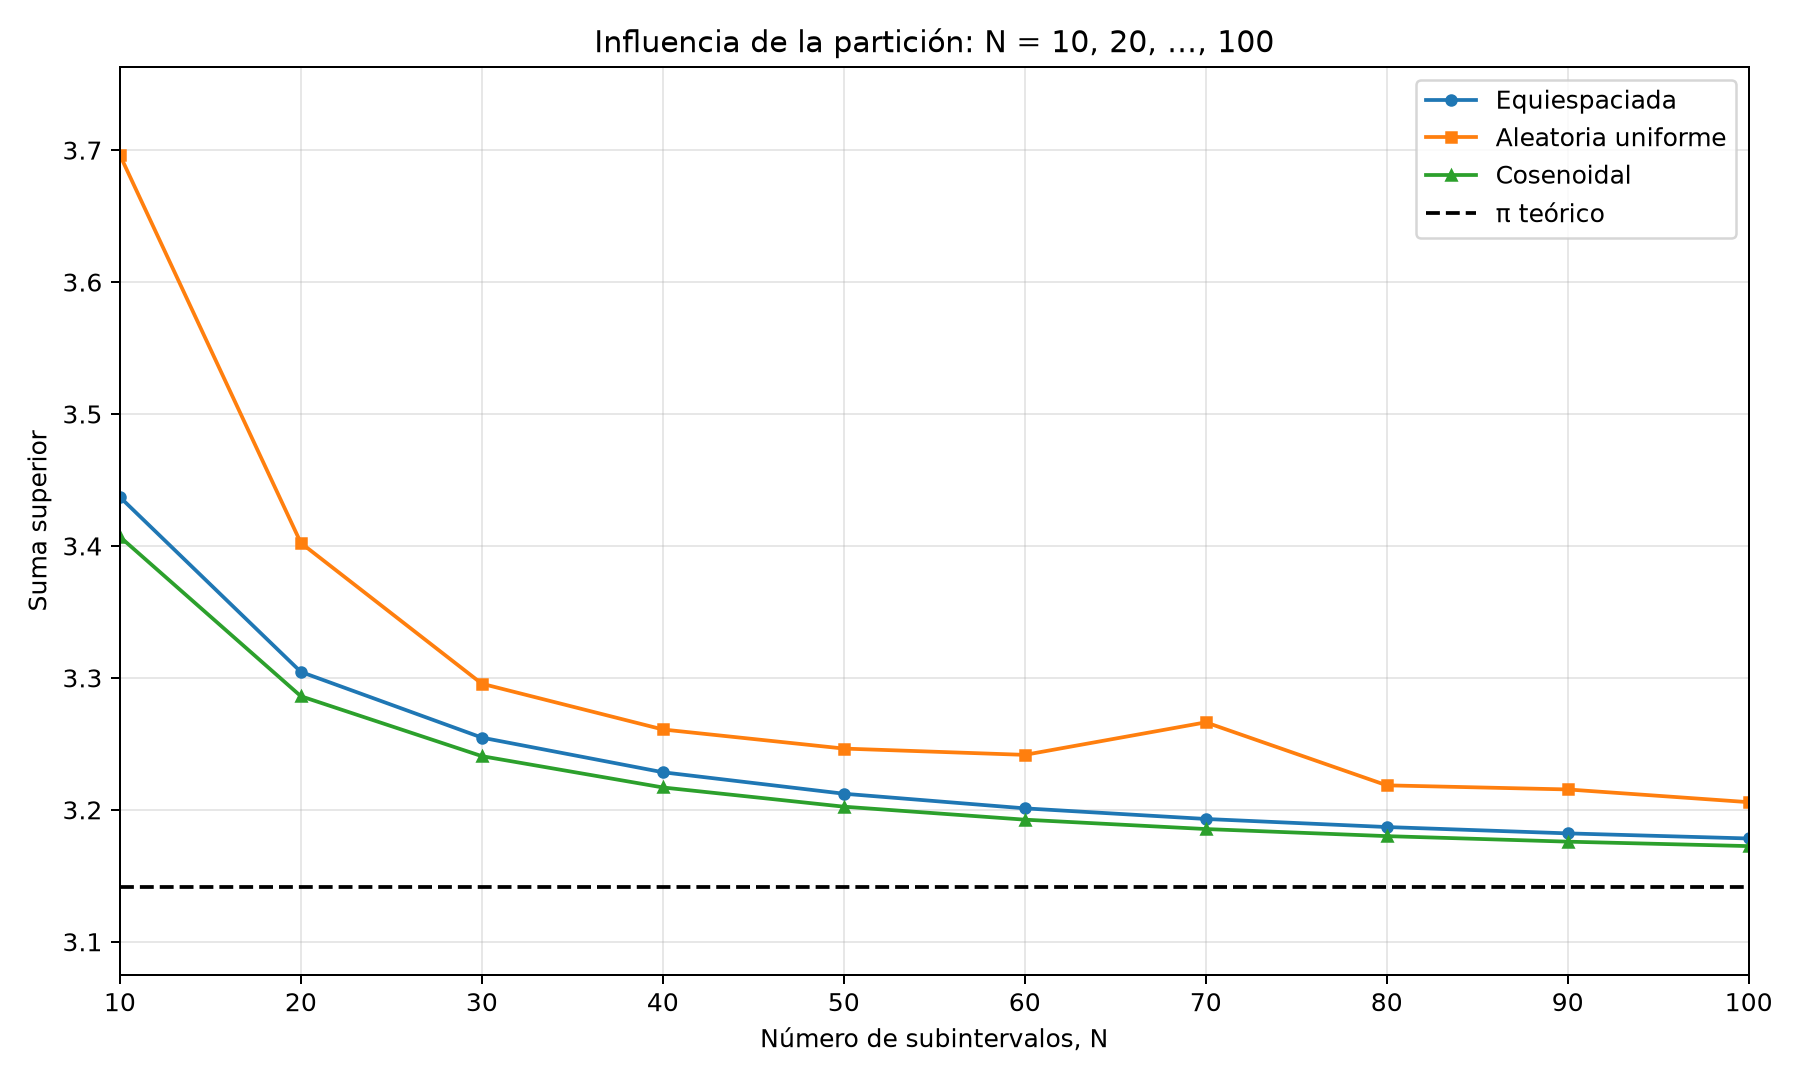
\includegraphics[width=0.88\textwidth]{2grafica_10_a_100.png}
\caption{Suma superior según el tipo de partición para \(N\) entre 10 y 100.}
\label{fig:e2_10a100}
\end{figure}

\begin{figure}[H]
\centering
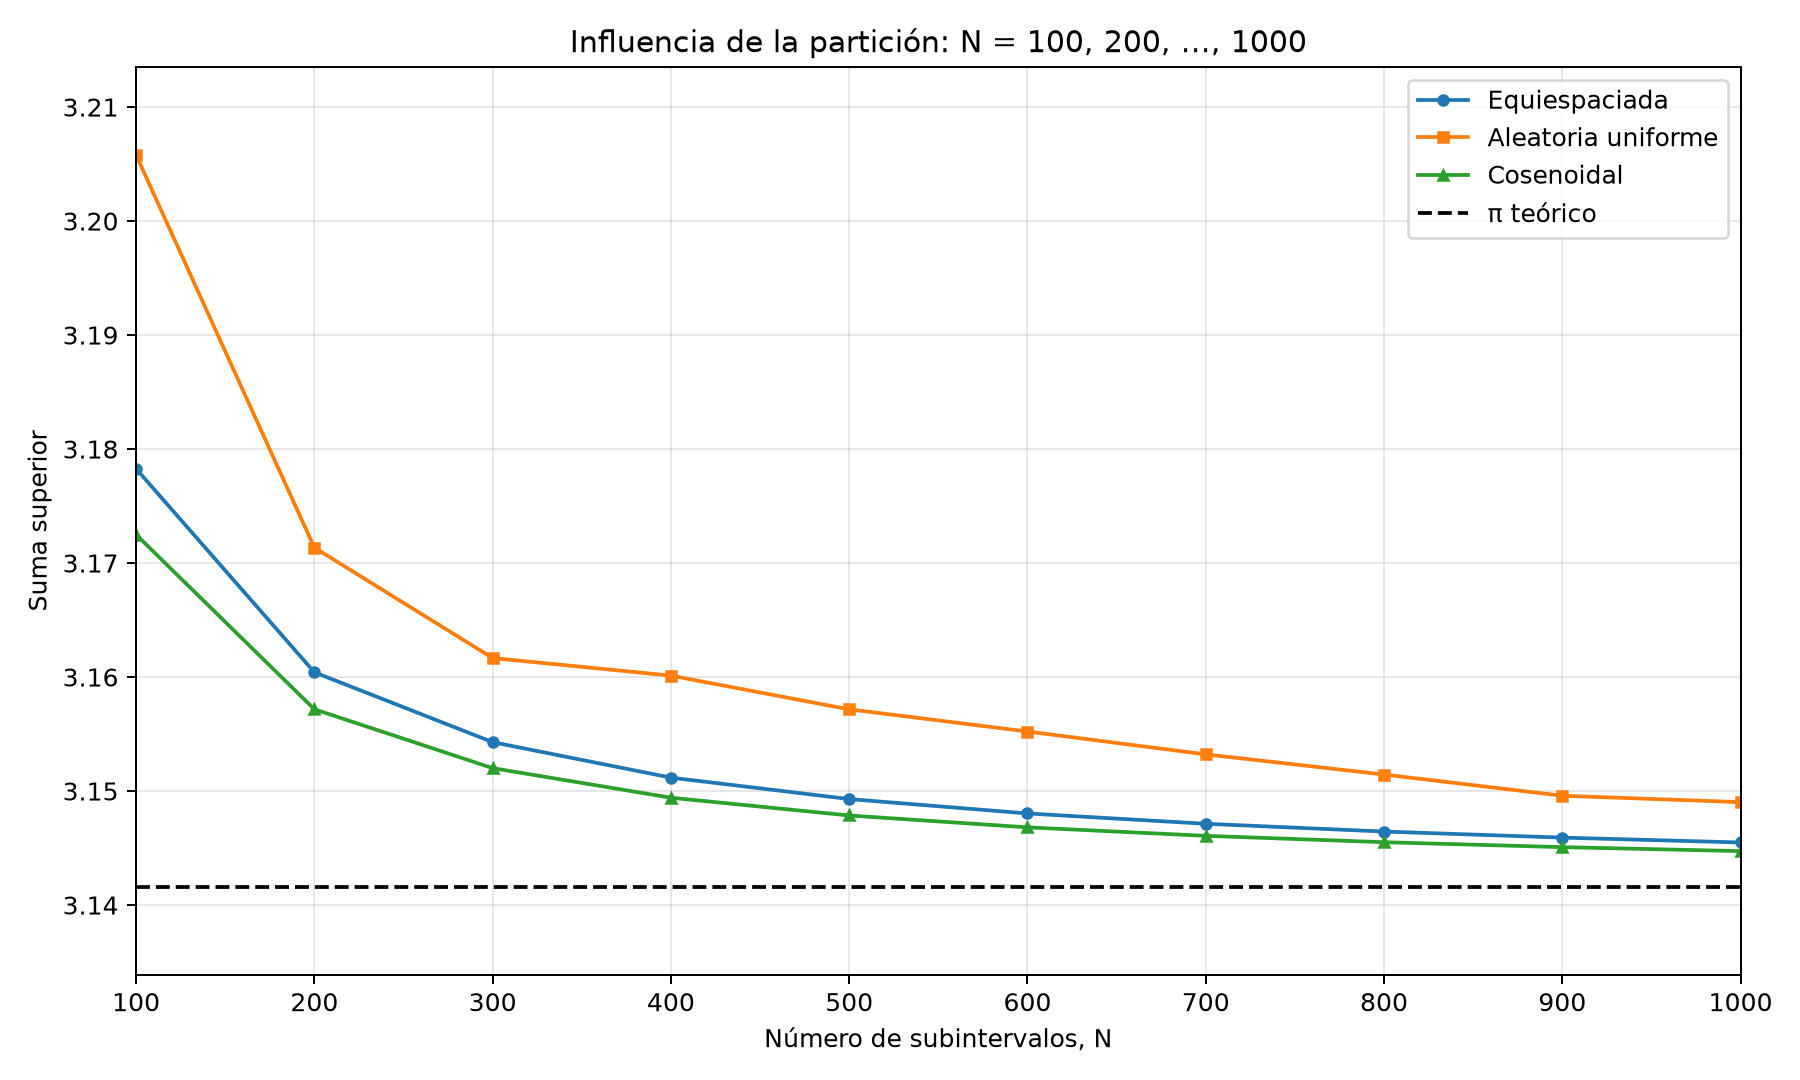
\includegraphics[width=0.88\textwidth]{2grafica_100_a_1000.png}
\caption{Suma superior según el tipo de partición para \(N\) entre 100 y 1000.}
\label{fig:e2_100a1000}
\end{figure}

\begin{figure}[H]
\centering
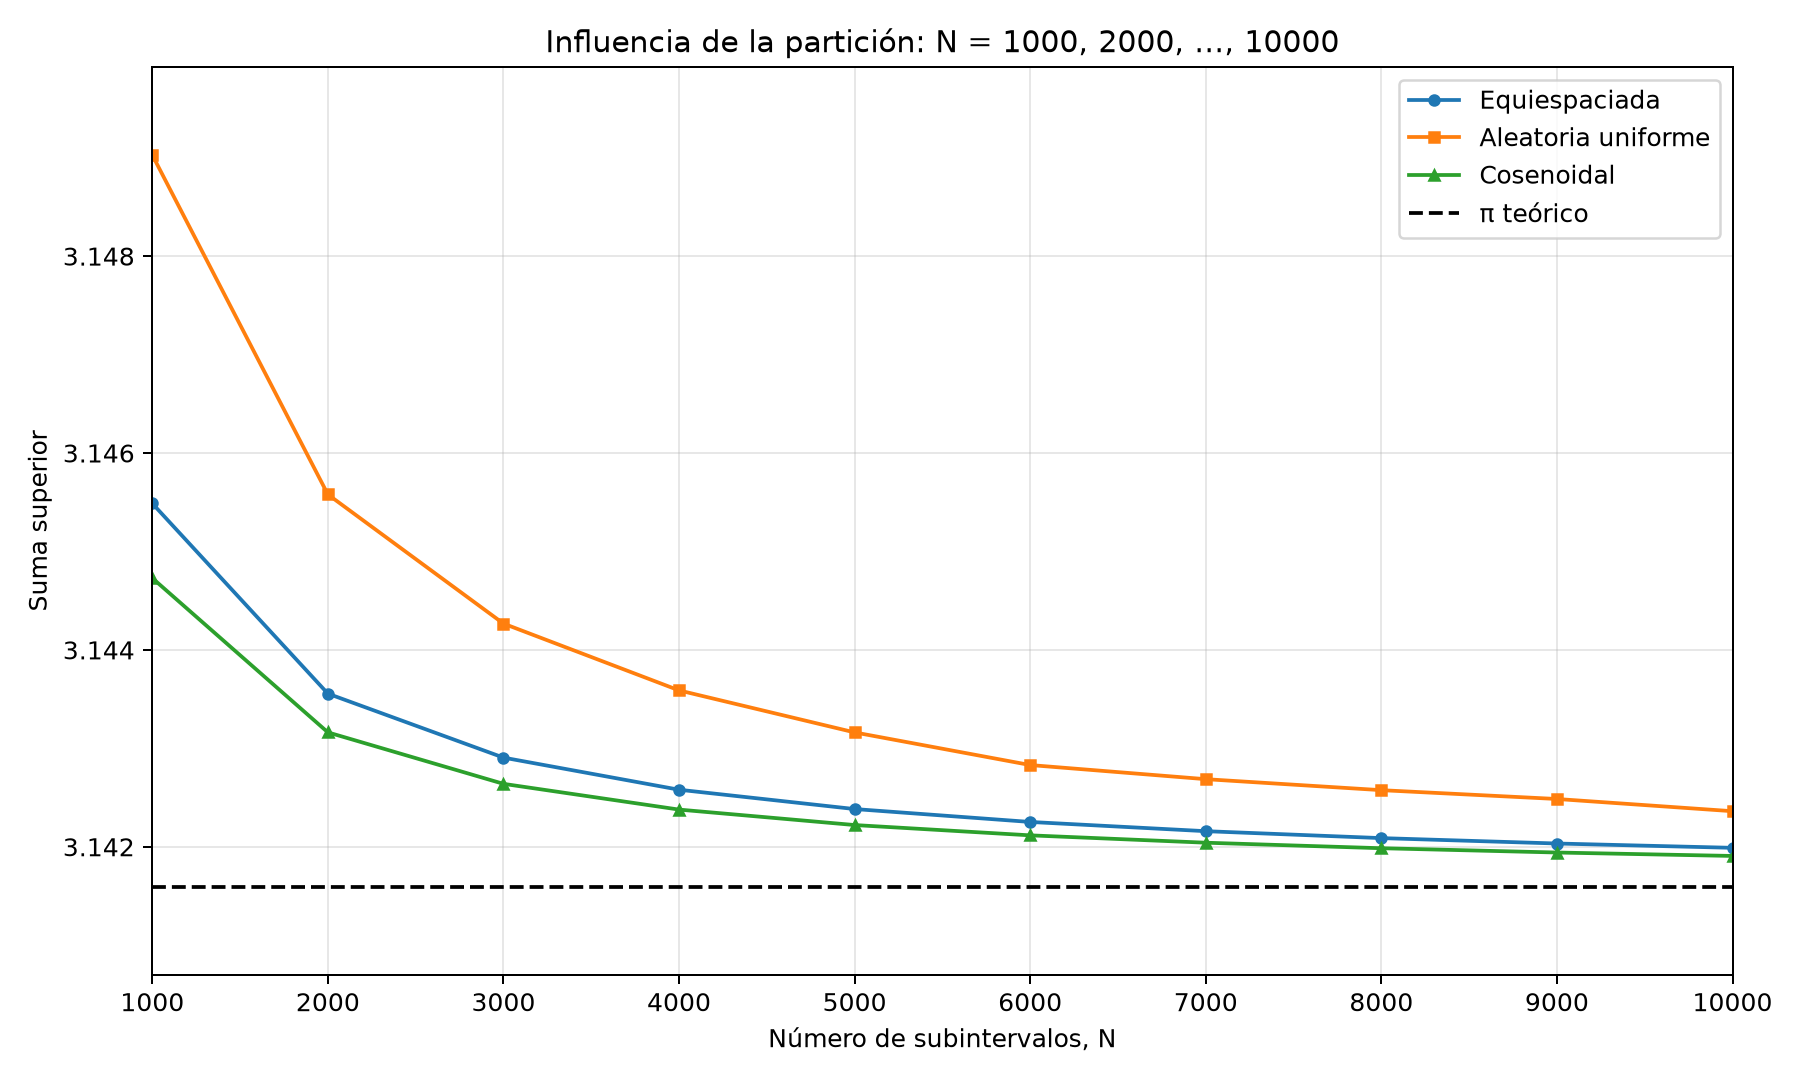
\includegraphics[width=0.88\textwidth]{2grafica_1000_a_10000.png}
\caption{Suma superior según el tipo de partición para \(N\) entre 1000 y 10000.}
\label{fig:e2_1000a10000}
\end{figure}

La consigna también pide graficar la función \(f\) y los rectángulos de la aproximación para cada partición con \(N=100\) (Figura~\ref{fig:e2_rect}). En la equiespaciada todos los rectángulos tienen el mismo ancho; en la aleatoria aparecen rectángulos muy finos junto a otros muy anchos, que sobresalen mucho de la curva; y en la cosenoidal los rectángulos son anchos en el centro y cada vez más finos hacia los bordes.

\begin{figure}[H]
\centering
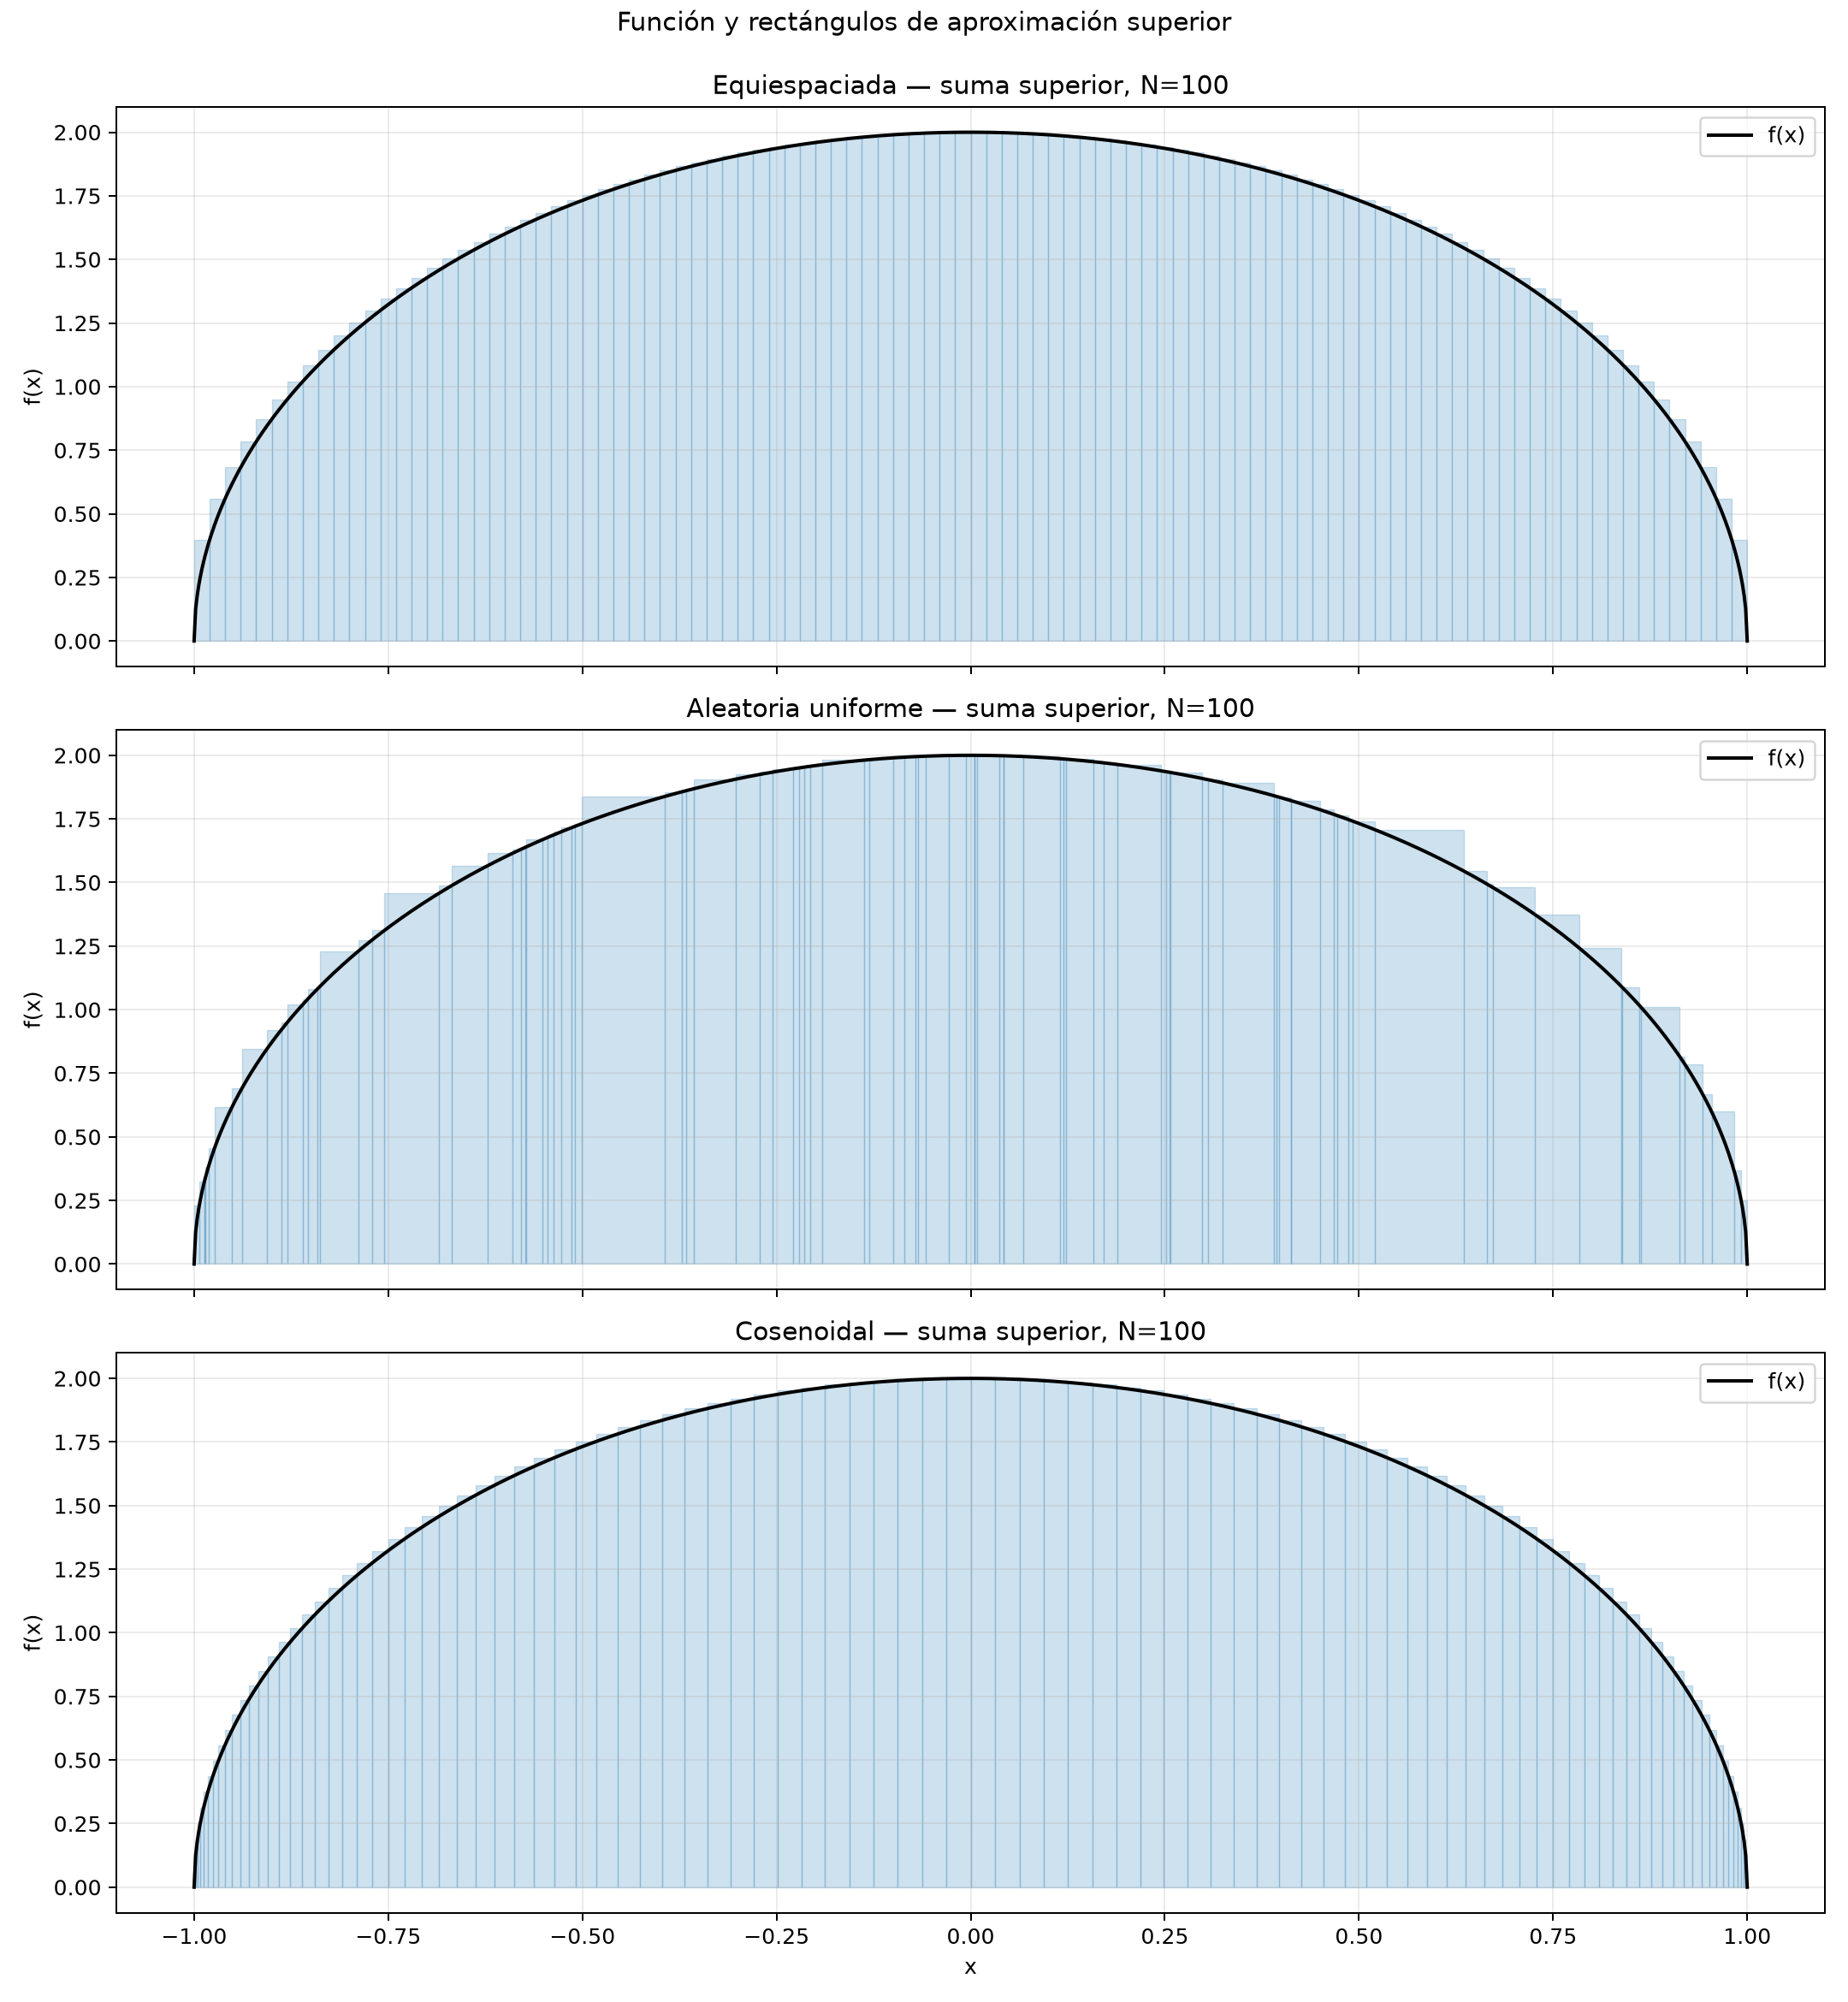
\includegraphics[width=0.85\textwidth]{2rectangulos_N100.png}
\caption{Función \(f\) y rectángulos de la suma superior para cada partición, con \(N=100\).}
\label{fig:e2_rect}
\end{figure}

\subsection{Conclusiones y respuestas analíticas}

\paragraph{¿Qué conclusiones puede tomar? ¿Hay particiones mejores que otras?}
Sí. Las tres particiones convergen a \(\pi\), pero no con la misma precisión: la cosenoidal tiene el menor error en todos los valores de \(N\), seguida por la equiespaciada. La aleatoria uniforme tiene un comportamiento irregular y un error consistentemente mayor (casi el doble que la equiespaciada), porque el azar siempre deja algunos subintervalos desproporcionadamente grandes. Hay que destacar que la mejora de la cosenoidal es moderada: su error es entre un 10\,\% (\(N=10\)) y un 21\,\% (\(N=10000\)) menor que el de la equiespaciada, y en las tres particiones el error disminuye aproximadamente como \(1/N\). Es decir, cambiar la partición reduce el error, pero no cambia la velocidad con la que converge el método.

\paragraph{¿Qué partición dio el mejor resultado? ¿Tiene sentido?}
La partición cosenoidal, \(x_i=\cos\left(\frac{i\pi}{N}\right)\). Tiene sentido: la función \(f(x)=2\sqrt{1-x^2}\) representa una semicircunferencia, cuya pendiente se vuelve vertical en los extremos \(x=\pm1\). En la suma superior, lo que sobra por encima de la curva en cada rectángulo depende de su ancho y de cuánto baja la curva dentro de él. Cerca de los bordes la curva baja muy rápido, así que ahí conviene usar rectángulos finos; en el centro la curva es casi plana y los rectángulos anchos casi no sobresalen. La partición cosenoidal hace exactamente eso: concentra los puntos en los bordes y los separa en el centro.

\paragraph{¿Afecta la geometría de la función a este resultado?}
Sí, la geometría es la explicación. La pendiente vertical en los extremos castiga a las particiones equiespaciada y aleatoria, que dejan subintervalos relativamente grandes justo donde la función cambia más. Los puntos cosenoidales provienen de dividir la circunferencia en ángulos iguales, por lo que se adaptan naturalmente a esta curva. Si la función fuera empinada en el centro y plana en los bordes, juntar los puntos en los extremos no ayudaría: no existe una partición que sea la mejor para todas las funciones, sino que conviene poner más puntos donde la función cambia más rápido.

%=====================================================================
\section{Ejercicio 3: Comparación de métodos}
%=====================================================================

\subsection{Introducción}

En esta sección comparamos tres métodos de integración numérica sobre una misma partición equiespaciada de \([-1,1]\). Como en el Ejercicio 1, \(N\) es la \textbf{cantidad de puntos} de la partición, que forman \(N-1\) subintervalos de ancho
\[
h=\frac{1-(-1)}{N-1}=\frac{2}{N-1},
\qquad x_i=-1+ih,\quad i=0,1,\ldots,N-1.
\]
Los tres métodos son:
\begin{enumerate}
    \item \textbf{Rectángulos (el método usual):} la altura de cada rectángulo es el valor de la función en el extremo izquierdo del subintervalo:
    \[
    R_N=h\sum_{i=0}^{N-2}f(x_i).
    \]
    \item \textbf{Trapecio:} en cada subintervalo se une con una recta los dos puntos de la curva en sus extremos, y se suma el área del trapecio que queda debajo:
    \[
    T_N=\sum_{i=0}^{N-2}\frac{f(x_i)+f(x_{i+1})}{2}\,h.
    \]
    \item \textbf{Punto medio:} la altura de cada rectángulo es el valor de la función en el centro del subintervalo:
    \[
    M_N=h\sum_{i=0}^{N-2}f\!\left(\frac{x_i+x_{i+1}}{2}\right).
    \]
\end{enumerate}
El residuo de cada método se define como \(Q_N-\pi\), donde \(Q_N\) es la aproximación. Un residuo negativo indica que el método subestima la integral y uno positivo, que la sobreestima; para comparar la precisión se mira su valor absoluto.

La Figura~\ref{fig:e3_ilustracion} muestra cómo aproxima el área cada método con solo \(N=6\) puntos.

\begin{figure}[H]
\centering
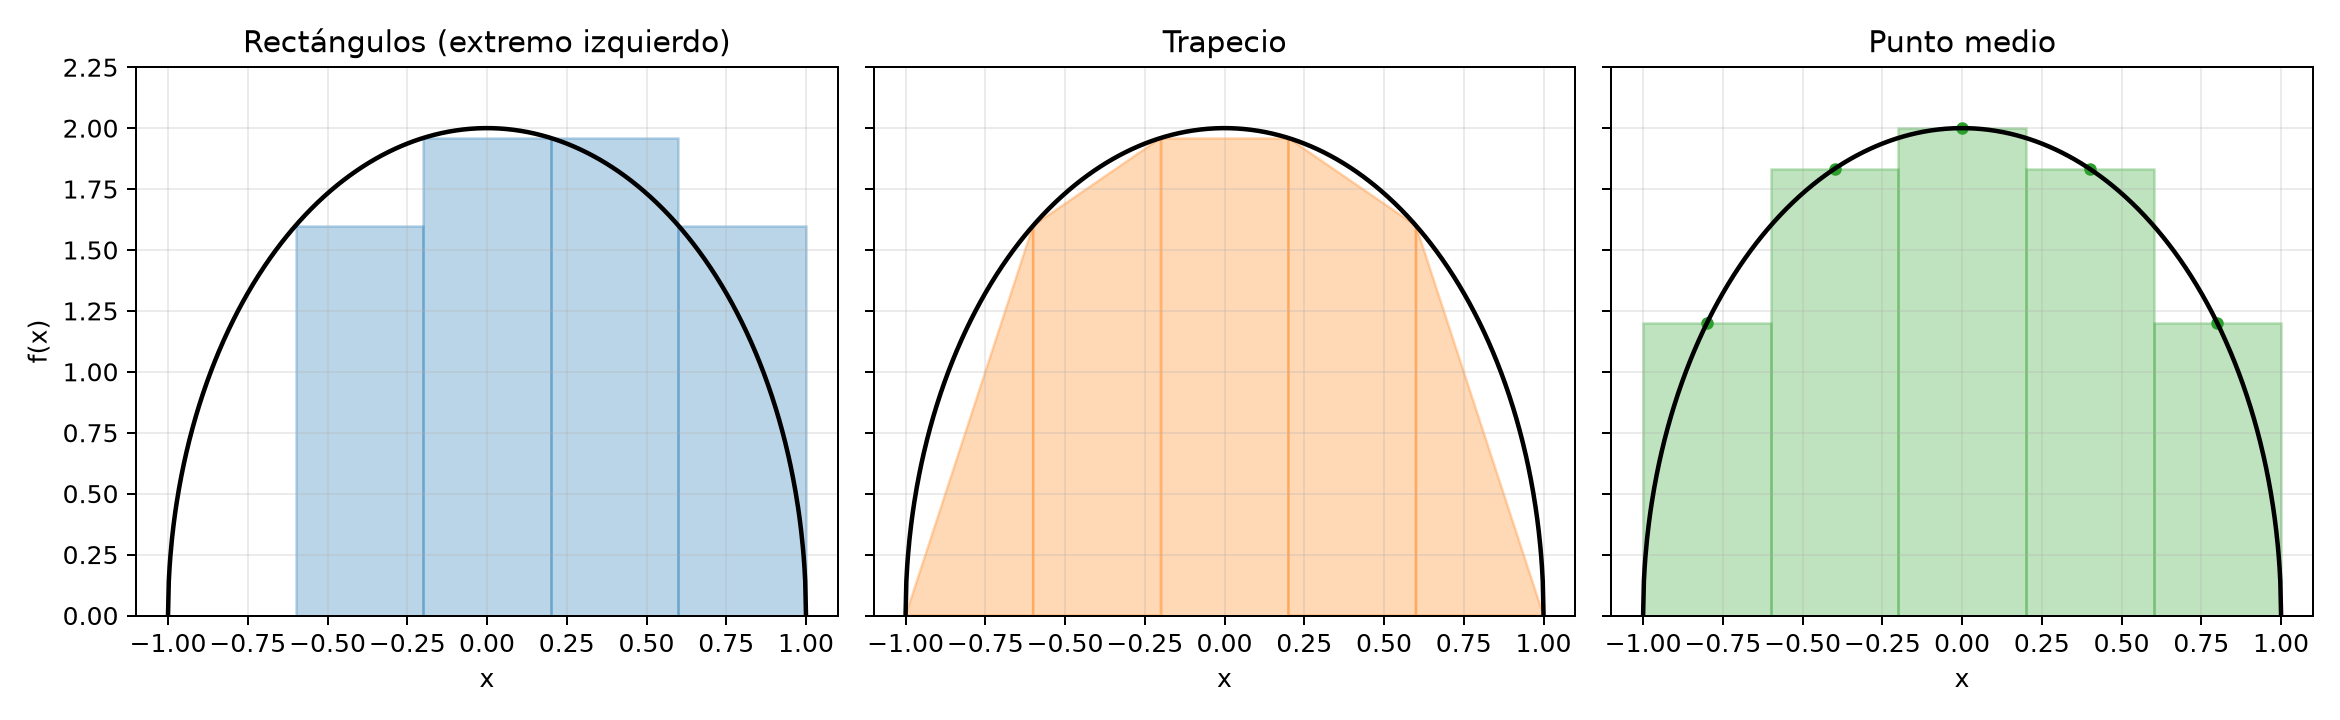
\includegraphics[width=\textwidth]{3metodos_ilustracion.png}
\caption{Aproximación del área con rectángulos (extremo izquierdo), trapecios y punto medio, con \(N=6\) puntos.}
\label{fig:e3_ilustracion}
\end{figure}

\subsection{Implementación en Python}

A continuación se muestra el código implementado en Python para construir la partición y calcular las tres aproximaciones (versión resumida; las funciones que imprimen las tablas, guardan los CSV y dibujan las gráficas se omiten):

\begin{lstlisting}[language=Python, caption={Código fuente del Ejercicio 3 (versión resumida)}]
import math

A = -1.0
B = 1.0
PI = math.pi

RANGOS_N = {
    "10_a_100": range(10, 101, 10),
    "100_a_1000": range(100, 1001, 100),
    "1000_a_10000": range(1000, 10001, 1000),
}

def f(x: float) -> float:
    return 2.0 * math.sqrt(max(0.0, 1.0 - x * x))

def particion_equiespaciada(n: int) -> list[float]:
    """N puntos equiespaciados, incluyendo -1 y 1 (N-1 subintervalos)."""
    if not isinstance(n, int) or isinstance(n, bool) or n < 2:
        raise ValueError("N debe ser un entero de al menos 2 puntos")
    return [A + (B - A) * i / (n - 1) for i in range(n)]

def metodo_rectangulos(puntos: list[float]) -> float:
    suma = 0.0
    for x_izq, x_der in zip(puntos, puntos[1:]):
        suma += f(x_izq) * (x_der - x_izq)
    return suma

def metodo_trapecio(puntos: list[float]) -> float:
    suma = 0.0
    for x_izq, x_der in zip(puntos, puntos[1:]):
        suma += (f(x_izq) + f(x_der)) * (x_der - x_izq) / 2.0
    return suma

def metodo_punto_medio(puntos: list[float]) -> float:
    suma = 0.0
    for x_izq, x_der in zip(puntos, puntos[1:]):
        punto_medio = (x_izq + x_der) / 2.0
        suma += f(punto_medio) * (x_der - x_izq)
    return suma

def generar_registros(valores_n: list[int]) -> list[dict[str, float | int]]:
    metodos = {
        "rectangulos": metodo_rectangulos,
        "trapecio": metodo_trapecio,
        "punto_medio": metodo_punto_medio,
    }
    registros = []
    for n in valores_n:
        puntos = particion_equiespaciada(n)
        registro: dict[str, float | int] = {"N": n}
        for nombre, funcion_metodo in metodos.items():
            aprox = funcion_metodo(puntos)
            registro[f"aprox_{nombre}"] = aprox
            registro[f"residuo_{nombre}"] = aprox - PI
        registros.append(registro)
    return registros
\end{lstlisting}

\subsection{Tablas comparativas de resultados}

Las siguientes tablas muestran la aproximación de cada método y su residuo. Como los residuos se hacen muy chicos, se escriben en notación científica.

\begin{table}[H]
\centering
\caption{Aproximación según el método, \(N\) entre 10 y 100, en incrementos de 10.}
\label{tab:e3_10a100}
\footnotesize
\setlength{\tabcolsep}{3pt}
\begin{tabular}{r r r r r r r}
\toprule
\(N\) & Rectángulos & Residuo & Trapecio & Residuo & Punto medio & Residuo \\
\midrule
10    & 3.01923183 & \(-1.2236\times10^{-1}\) & 3.01923183 & \(-1.2236\times10^{-1}\) & 3.17713893 & \(+3.5546\times10^{-2}\) \\
20    & 3.10155965 & \(-4.0033\times10^{-2}\) & 3.10155965 & \(-4.0033\times10^{-2}\) & 3.15327255 & \(+1.1680\times10^{-2}\) \\
30    & 3.12033906 & \(-2.1254\times10^{-2}\) & 3.12033906 & \(-2.1254\times10^{-2}\) & 3.14780184 & \(+6.2092\times10^{-3}\) \\
40    & 3.12795728 & \(-1.3635\times10^{-2}\) & 3.12795728 & \(-1.3635\times10^{-2}\) & 3.14557880 & \(+3.9861\times10^{-3}\) \\
50    & 3.13190745 & \(-9.6852\times10^{-3}\) & 3.13190745 & \(-9.6852\times10^{-3}\) & 3.14442511 & \(+2.8325\times10^{-3}\) \\
60    & 3.13426075 & \(-7.3319\times10^{-3}\) & 3.13426075 & \(-7.3319\times10^{-3}\) & 3.14373743 & \(+2.1448\times10^{-3}\) \\
70    & 3.13579454 & \(-5.7981\times10^{-3}\) & 3.13579454 & \(-5.7981\times10^{-3}\) & 3.14328906 & \(+1.6964\times10^{-3}\) \\
80    & 3.13685931 & \(-4.7333\times10^{-3}\) & 3.13685931 & \(-4.7333\times10^{-3}\) & 3.14297772 & \(+1.3851\times10^{-3}\) \\
90    & 3.13763387 & \(-3.9588\times10^{-3}\) & 3.13763387 & \(-3.9588\times10^{-3}\) & 3.14275119 & \(+1.1585\times10^{-3}\) \\
100   & 3.13821804 & \(-3.3746\times10^{-3}\) & 3.13821804 & \(-3.3746\times10^{-3}\) & 3.14258032 & \(+9.8766\times10^{-4}\) \\
\bottomrule
\end{tabular}
\end{table}

\begin{table}[H]
\centering
\caption{Aproximación según el método, \(N\) entre 100 y 1000, en incrementos de 100.}
\label{tab:e3_100a1000}
\footnotesize
\setlength{\tabcolsep}{3pt}
\begin{tabular}{r r r r r r r}
\toprule
\(N\) & Rectángulos & Residuo & Trapecio & Residuo & Punto medio & Residuo \\
\midrule
100   & 3.13821804 & \(-3.3746\times10^{-3}\) & 3.13821804 & \(-3.3746\times10^{-3}\) & 3.14258032 & \(+9.8766\times10^{-4}\) \\
200   & 3.14040816 & \(-1.1845\times10^{-3}\) & 3.14040816 & \(-1.1845\times10^{-3}\) & 3.14193945 & \(+3.4680\times10^{-4}\) \\
300   & 3.14094945 & \(-6.4321\times10^{-4}\) & 3.14094945 & \(-6.4321\times10^{-4}\) & 3.14178100 & \(+1.8834\times10^{-4}\) \\
400   & 3.14117538 & \(-4.1727\times10^{-4}\) & 3.14117538 & \(-4.1727\times10^{-4}\) & 3.14171485 & \(+1.2219\times10^{-4}\) \\
500   & 3.14129429 & \(-2.9836\times10^{-4}\) & 3.14129429 & \(-2.9836\times10^{-4}\) & 3.14168003 & \(+8.7375\times10^{-5}\) \\
600   & 3.14136579 & \(-2.2686\times10^{-4}\) & 3.14136579 & \(-2.2686\times10^{-4}\) & 3.14165909 & \(+6.6438\times10^{-5}\) \\
700   & 3.14141269 & \(-1.7997\times10^{-4}\) & 3.14141269 & \(-1.7997\times10^{-4}\) & 3.14164536 & \(+5.2705\times10^{-5}\) \\
800   & 3.14144539 & \(-1.4726\times10^{-4}\) & 3.14144539 & \(-1.4726\times10^{-4}\) & 3.14163578 & \(+4.3128\times10^{-5}\) \\
900   & 3.14146926 & \(-1.2339\times10^{-4}\) & 3.14146926 & \(-1.2339\times10^{-4}\) & 3.14162879 & \(+3.6137\times10^{-5}\) \\
1000  & 3.14148732 & \(-1.0533\times10^{-4}\) & 3.14148732 & \(-1.0533\times10^{-4}\) & 3.14162350 & \(+3.0849\times10^{-5}\) \\
\bottomrule
\end{tabular}
\end{table}

\begin{table}[H]
\centering
\caption{Aproximación según el método, \(N\) entre 1000 y 10000, en incrementos de 1000.}
\label{tab:e3_1000a10000}
\footnotesize
\setlength{\tabcolsep}{3pt}
\begin{tabular}{r r r r r r r}
\toprule
\(N\) & Rectángulos & Residuo & Trapecio & Residuo & Punto medio & Residuo \\
\midrule
1000  & 3.14148732 & \(-1.0533\times10^{-4}\) & 3.14148732 & \(-1.0533\times10^{-4}\) & 3.14162350 & \(+3.0849\times10^{-5}\) \\
2000  & 3.14155544 & \(-3.7215\times10^{-5}\) & 3.14155544 & \(-3.7215\times10^{-5}\) & 3.14160355 & \(+1.0899\times10^{-5}\) \\
3000  & 3.14157240 & \(-2.0252\times10^{-5}\) & 3.14157240 & \(-2.0252\times10^{-5}\) & 3.14159859 & \(+5.9316\times10^{-6}\) \\
4000  & 3.14157950 & \(-1.3153\times10^{-5}\) & 3.14157950 & \(-1.3153\times10^{-5}\) & 3.14159651 & \(+3.8522\times10^{-6}\) \\
5000  & 3.14158324 & \(-9.4106\times10^{-6}\) & 3.14158324 & \(-9.4106\times10^{-6}\) & 3.14159541 & \(+2.7562\times10^{-6}\) \\
6000  & 3.14158550 & \(-7.1585\times10^{-6}\) & 3.14158550 & \(-7.1585\times10^{-6}\) & 3.14159475 & \(+2.0967\times10^{-6}\) \\
7000  & 3.14158697 & \(-5.6805\times10^{-6}\) & 3.14158697 & \(-5.6805\times10^{-6}\) & 3.14159432 & \(+1.6638\times10^{-6}\) \\
8000  & 3.14158800 & \(-4.6493\times10^{-6}\) & 3.14158800 & \(-4.6493\times10^{-6}\) & 3.14159402 & \(+1.3617\times10^{-6}\) \\
9000  & 3.14158876 & \(-3.8963\times10^{-6}\) & 3.14158876 & \(-3.8963\times10^{-6}\) & 3.14159379 & \(+1.1412\times10^{-6}\) \\
10000 & 3.14158933 & \(-3.3267\times10^{-6}\) & 3.14158933 & \(-3.3267\times10^{-6}\) & 3.14159363 & \(+9.7435\times10^{-7}\) \\
\bottomrule
\end{tabular}
\end{table}

Lo primero que llama la atención es que \textbf{rectángulos y trapecio dan exactamente el mismo resultado} en todas las filas. No es un error del programa: como \(f(-1)=f(1)=0\), el primer rectángulo tiene altura cero, y en la fórmula del trapecio los dos extremos también aportan cero, así que las dos fórmulas terminan sumando exactamente los mismos términos:
\[
R_N=h\sum_{i=1}^{N-2}f(x_i)=T_N.
\]
Además, rectángulos y trapecio siempre quedan por debajo de \(\pi\) (residuo negativo), mientras que el punto medio siempre queda por encima (residuo positivo) y con un error absoluto unas tres veces menor.

\subsection{Análisis de las gráficas}

Las gráficas muestran las tres aproximaciones junto con el valor exacto \(\pi\) para cada rango de \(N\). Las curvas de rectángulos y trapecio aparecen superpuestas porque sus valores coinciden.

\begin{figure}[H]
\centering
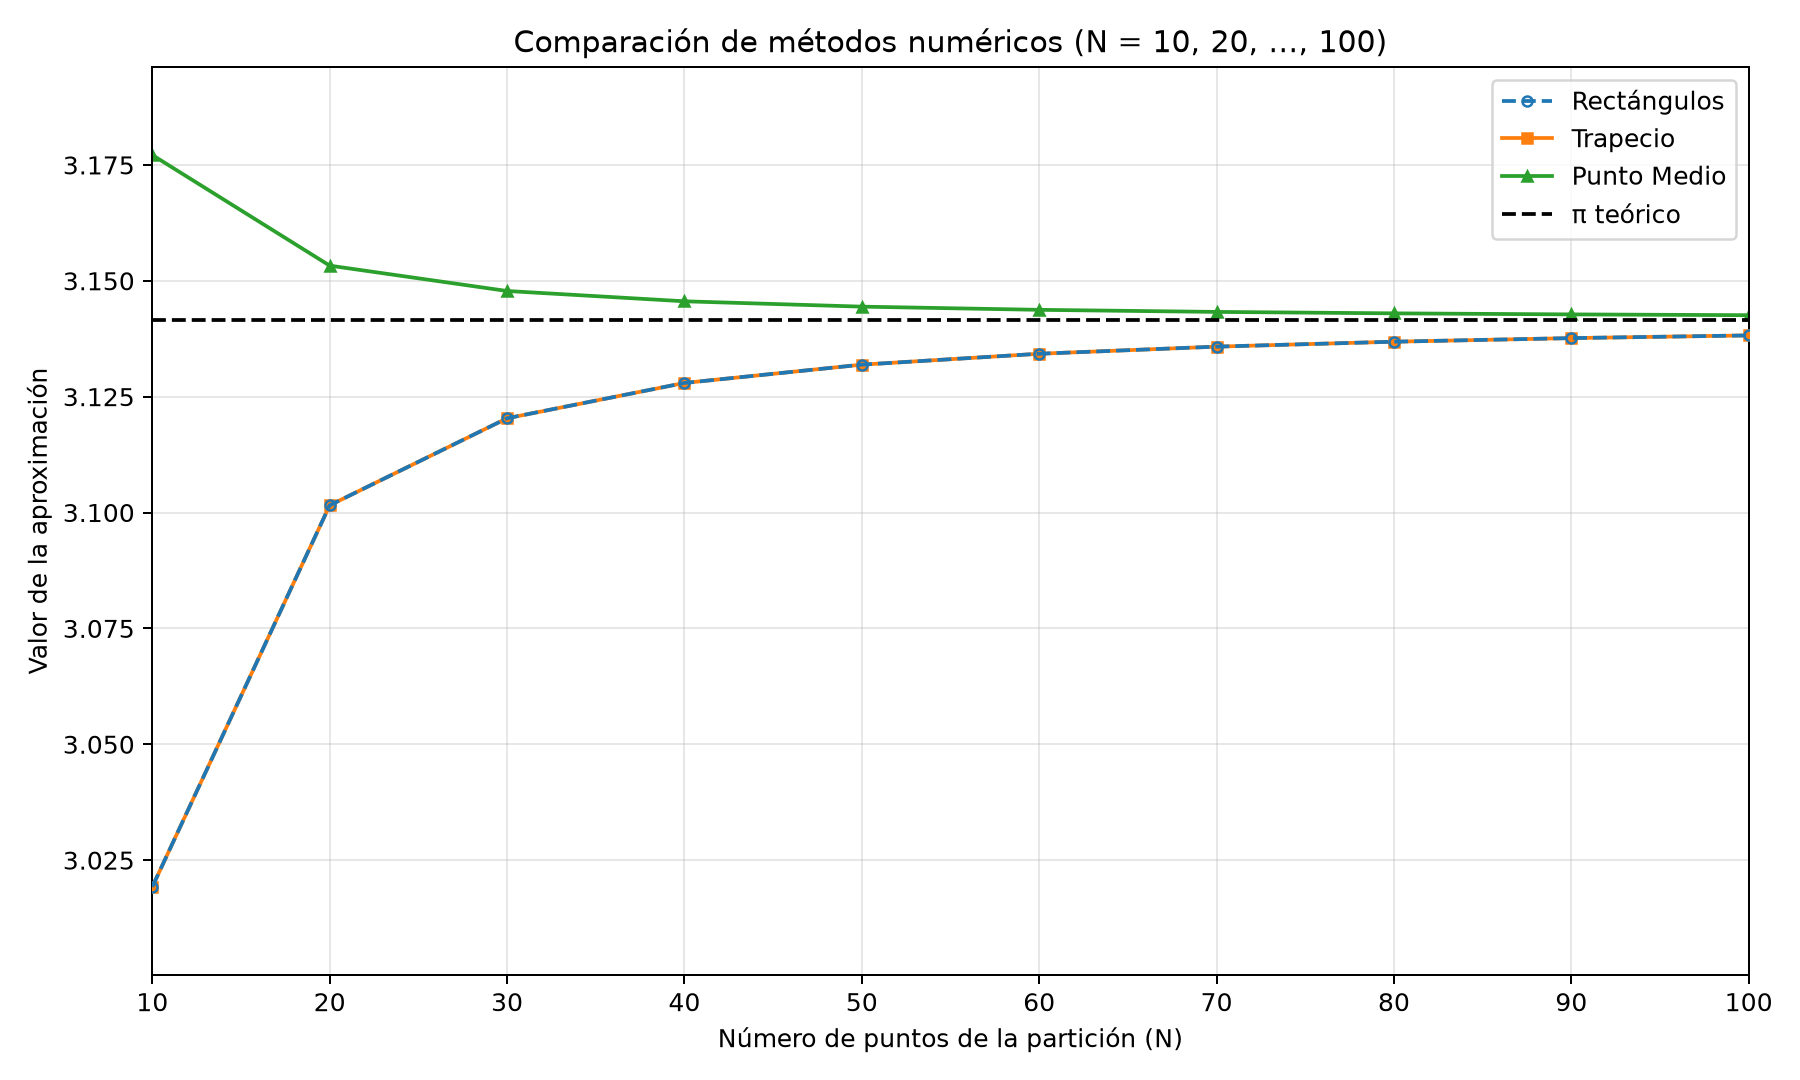
\includegraphics[width=0.88\textwidth]{3grafica_metodos_10_a_100.png}
\caption{Aproximación según el método para \(N\) entre 10 y 100.}
\label{fig:e3_10a100}
\end{figure}

\begin{figure}[H]
\centering
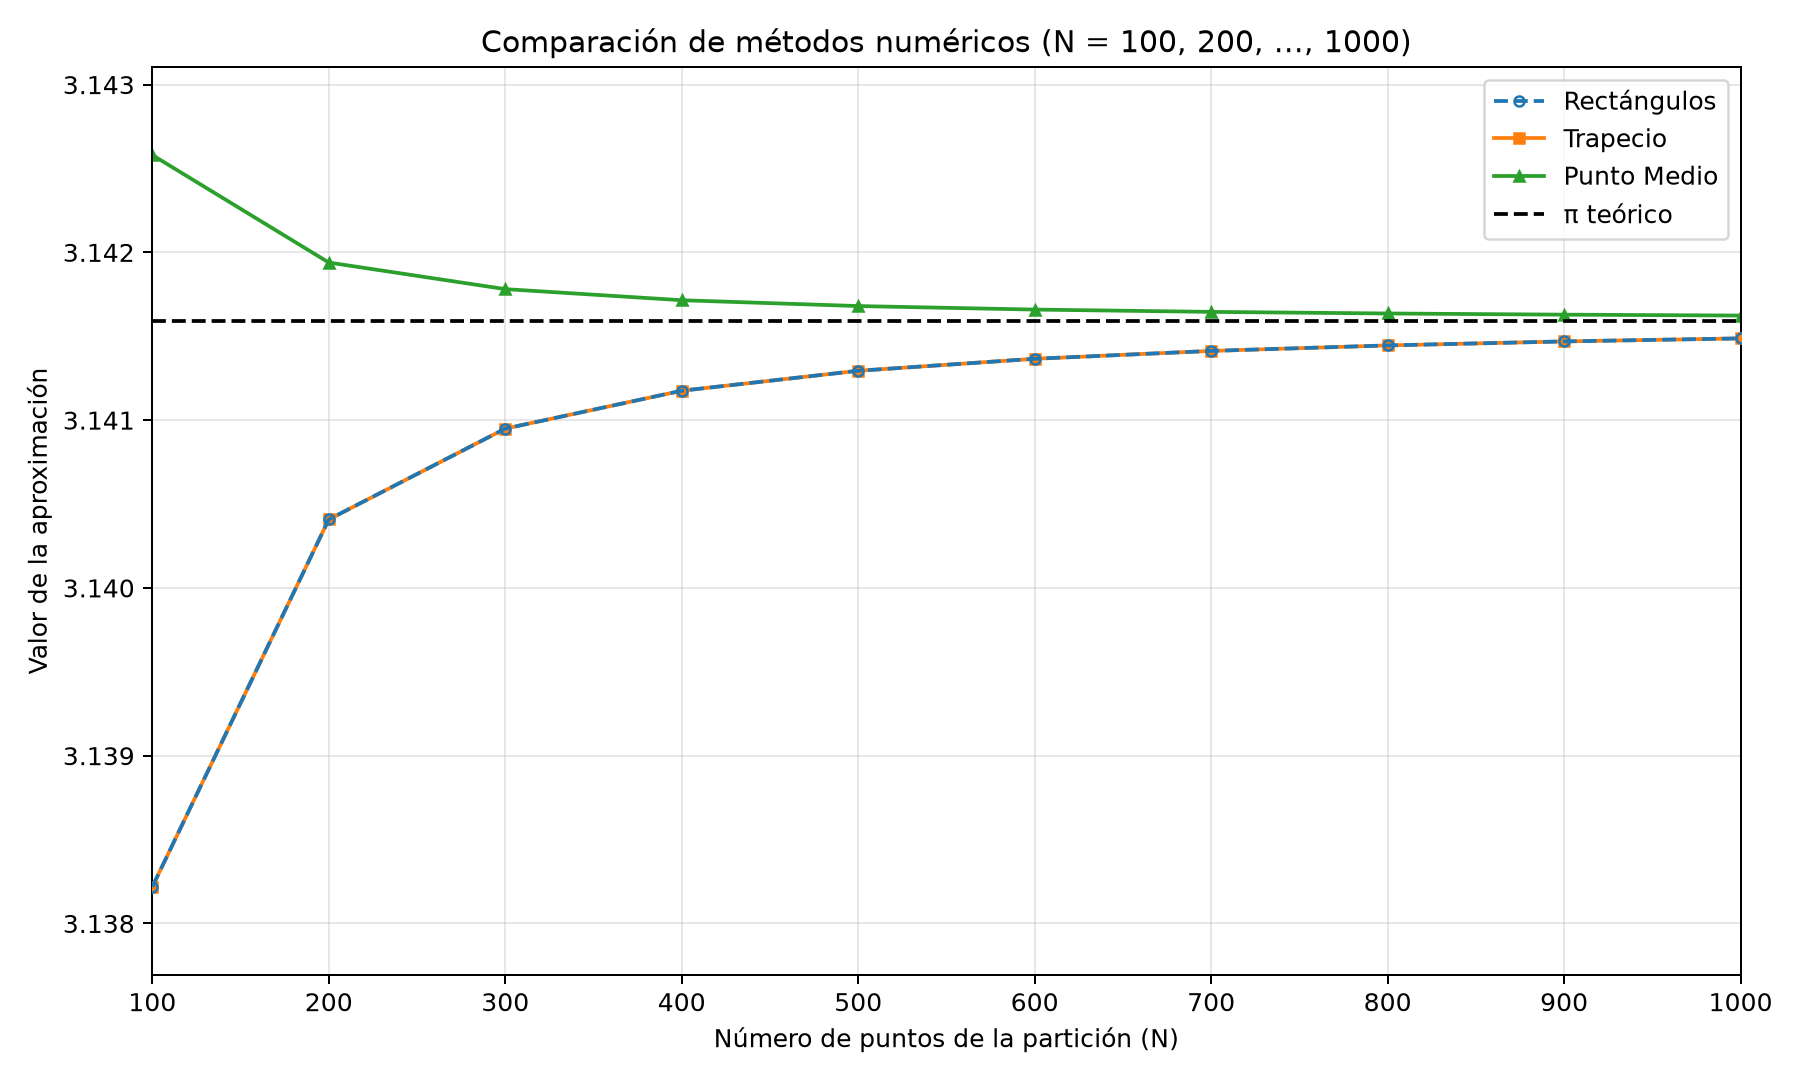
\includegraphics[width=0.88\textwidth]{3grafica_metodos_100_a_1000.png}
\caption{Aproximación según el método para \(N\) entre 100 y 1000.}
\label{fig:e3_100a1000}
\end{figure}

\begin{figure}[H]
\centering
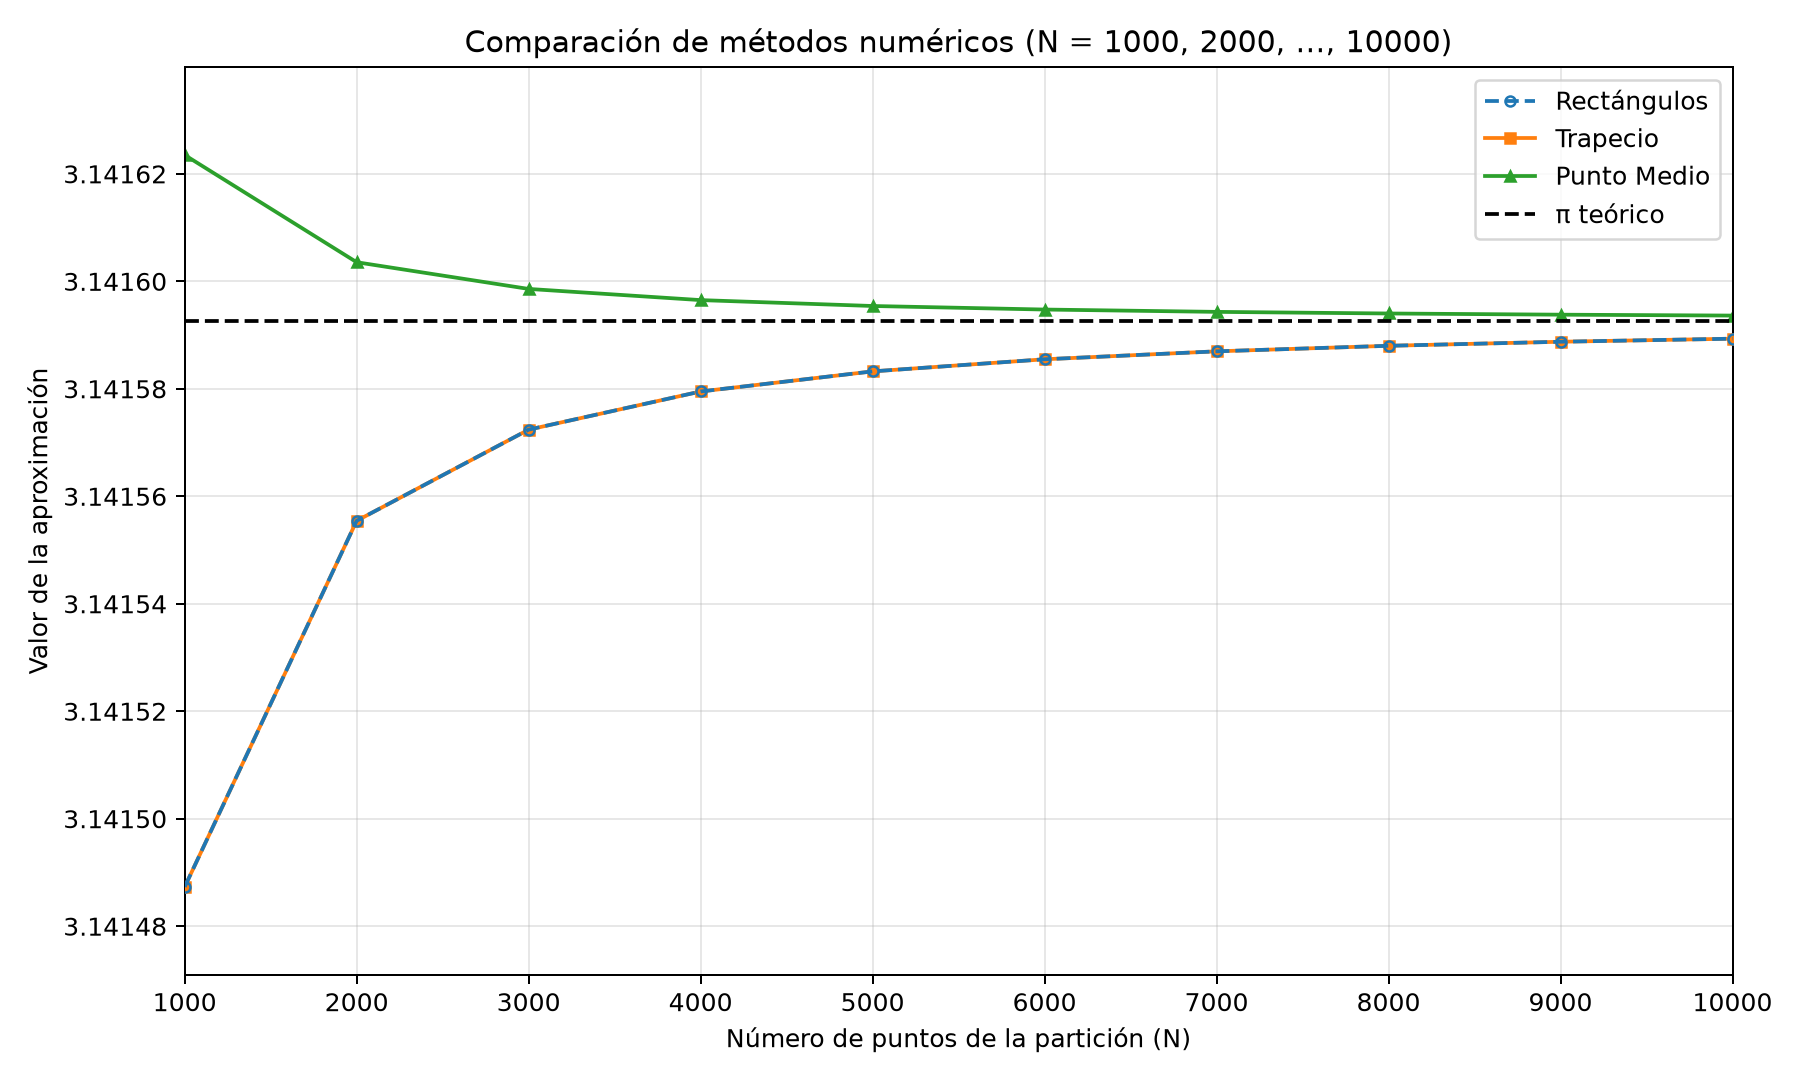
\includegraphics[width=0.88\textwidth]{3grafica_metodos_1000_a_10000.png}
\caption{Aproximación según el método para \(N\) entre 1000 y 10000.}
\label{fig:e3_1000a10000}
\end{figure}

Para ver mejor qué tan rápido baja el error, la Figura~\ref{fig:e3_log} muestra el valor absoluto del residuo en escala logarítmica (cada marca de los ejes representa multiplicar por 10).

\begin{figure}[H]
\centering
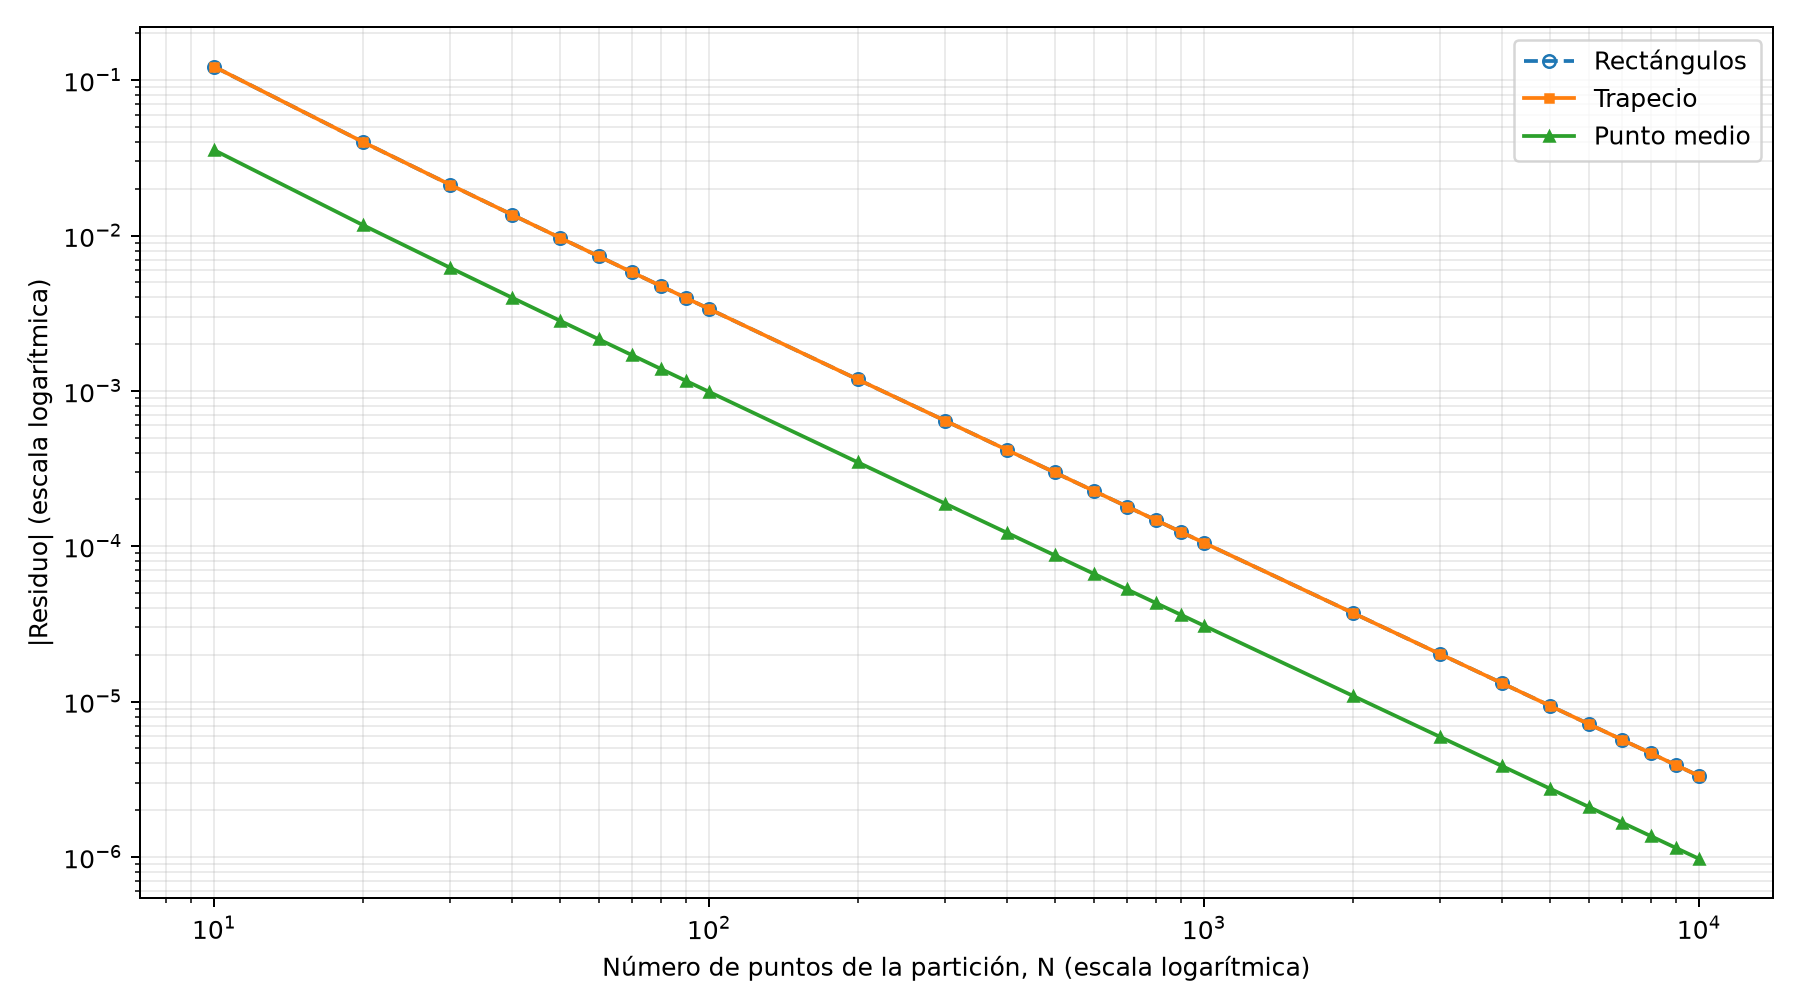
\includegraphics[width=0.88\textwidth]{3errores_log.png}
\caption{Valor absoluto del residuo de cada método según \(N\), en escala logarítmica.}
\label{fig:e3_log}
\end{figure}

Las tres líneas son rectas y paralelas: cada vez que \(N\) se multiplica por 10, el error se divide aproximadamente por 32 (por ejemplo, el residuo del trapecio pasa de \(3.37\times10^{-3}\) con \(N=100\) a \(1.05\times10^{-4}\) con \(N=1000\)). Esto es mucho mejor que las sumas de Darboux de los Ejercicios 1 y 2, donde el error solo se dividía por 10. Con \(N=10000\), el trapecio tiene un error de \(3.3\times10^{-6}\), unas 100 veces menor que el de la suma superior con la misma partición (\(4.0\times10^{-4}\)).

\subsection{Conclusiones y respuestas analíticas}

\paragraph{¿Qué método dio mejores resultados?}
El \textbf{punto medio}. En todos los valores de \(N\) su residuo es el más chico en valor absoluto: aproximadamente un 29\,\% del error del trapecio (por ejemplo, \(9.88\times10^{-4}\) contra \(3.37\times10^{-3}\) con \(N=100\)). Rectángulos y trapecio quedan empatados, porque en este problema dan exactamente el mismo resultado.

\paragraph{¿Hay métodos mejores que otros?}
Sí, pero hay que matizarlo. En general, el trapecio es mejor que los rectángulos, porque reemplaza la ``escalera'' de rectángulos por segmentos que siguen la inclinación de la curva. En este ejercicio esa ventaja no se ve, porque la función vale cero en los dos extremos del intervalo y las dos fórmulas coinciden. Si la función no se anulara en los extremos, los resultados serían distintos. El punto medio, en cambio, sí resulta mejor que los otros dos para esta función.

\paragraph{Justificación geométrica.}
La clave es que la función es \textbf{cóncava hacia abajo} (tiene forma de cúpula):
\[
f''(x)=-\frac{2}{(1-x^2)^{3/2}}<0,\qquad -1<x<1.
\]
\begin{itemize}
    \item \textbf{Trapecio:} el lado de arriba de cada trapecio es una cuerda que une dos puntos de la curva. En una curva cóncava hacia abajo, las cuerdas quedan siempre \textbf{por debajo} de la curva, así que cada trapecio deja un pequeño hueco sin cubrir y la suma total queda por debajo de \(\pi\) (Figura~\ref{fig:e3_ilustracion}, centro).
    \item \textbf{Punto medio:} el área del rectángulo de punto medio es igual al área del trapecio que se forma con la \textbf{recta tangente} a la curva en el centro del subintervalo (lo que el rectángulo agrega de un lado de la tangente lo quita del otro). En una curva cóncava hacia abajo, la tangente queda \textbf{por encima} de la curva, así que el punto medio sobreestima la integral y su residuo es positivo.
    \item \textbf{¿Por qué el punto medio se equivoca menos?} Cerca del centro del subintervalo, la tangente se ``pega'' a la curva mucho más que la cuerda, que solo la toca en los extremos. Por eso el espacio entre la tangente y la curva es más chico que el espacio entre la cuerda y la curva. En funciones suaves el error del punto medio suele ser la mitad del error del trapecio; en nuestra función resultó todavía menor (alrededor del 29\,\%).
\end{itemize}

Por último, el error de los tres métodos baja a un ritmo de aproximadamente \(N^{-1.5}\) (dividido por 32 cada vez que \(N\) se multiplica por 10), y no como \(N^{-2}\), que es lo habitual para el trapecio y el punto medio. Esto también se explica por la geometría: en los extremos \(x=\pm1\) la curva cae en vertical, y ahí ninguna recta (ni la cuerda ni la tangente) la puede seguir bien, así que la mayor parte del error se concentra en los subintervalos de los bordes.

%=====================================================================
\section{Conclusiones generales}
%=====================================================================

En los tres ejercicios aproximamos \(\pi\) como el área bajo \(f(x)=2\sqrt{1-x^2}\), y todos los métodos convergieron al valor exacto al aumentar \(N\), como corresponde a una función continua e integrable de Riemann. Sin embargo, no todas las estrategias mejoran igual. Cambiar la forma de la partición (Ejercicio 2) redujo el error de la suma superior entre un 10\,\% y un 21\,\%, pero mantuvo el mismo ritmo de convergencia que en el Ejercicio 1, donde el error se dividía por 10 cada vez que \(N\) se multiplicaba por 10. En cambio, cambiar la forma de calcular el área de cada subintervalo (Ejercicio 3) cambió el ritmo: con trapecio y punto medio el error se dividió por 32, y el punto medio fue el método más preciso de todos los que probamos.

%=====================================================================
\section*{Referencias}
\addcontentsline{toc}{section}{Referencias}
%=====================================================================

\begingroup
\setlength{\parindent}{-1.27cm}
\setlength{\leftskip}{1.27cm}
\setlength{\parskip}{6pt}

Hunter, J. D. (2007). Matplotlib: A 2D graphics environment. \textit{Computing in Science \& Engineering, 9}(3), 90--95. \url{https://doi.org/10.1109/MCSE.2007.55}

Python Software Foundation. (s.f.). \textit{Python} [Software]. \url{https://www.python.org}

Stewart, J. (2012). \textit{Cálculo de una variable: Trascendentes tempranas} (7.ª ed.; M. C. Rodríguez Pedroza, Trad.). Cengage Learning.

Universidad Católica del Uruguay. (2026). \textit{Comparación de métodos de integración numérica} [Consigna del proyecto grupal, Cálculo Aplicado]. Facultad de Ingeniería y Tecnología.

\endgroup

%=====================================================================

% Los bloques de código se llaman "Código 1, 2, 3" en lugar de "Listing"
\renewcommand{\lstlistingname}{Código}

%=====================================================================
\section{Ejercicio 1: Convergencia de las sumas inferior y superior}
%=====================================================================

\subsection{Introducción y análisis teórico}

La función y el intervalo bajo estudio son:
\[
f(x)=2\sqrt{1-x^2}, \qquad x\in[-1,1].
\]

La ecuación \(x^2+y^2=1\) describe el círculo unitario. Su semicircunferencia superior corresponde a \(y=\sqrt{1-x^2}\). La función del ejercicio es el doble de dicha altura, es decir, \(f(x)=2y\). El área de la semicircunferencia unitaria es \(\pi/2\); al duplicar las alturas, el área exacta bajo la curva es:
\[
\int_{-1}^{1}2\sqrt{1-x^2}\,dx=\pi.
\]

\subsection{Cómo se forman las sumas}

Para un valor de \(N\), se consideran \(N\) puntos equiespaciados, que generan \(N-1\) subintervalos de igual ancho:
\[
\Delta x=\frac{1-(-1)}{N-1}=\frac{2}{N-1}.
\]
Los puntos de la partición son \(x_i=-1+i\Delta x\), para \(i=0,1,\ldots,N-1\). Si \(m_i\) y \(M_i\) son, respectivamente, el mínimo y el máximo de la función en cada subintervalo, las sumas de Darboux son:
\[
L_N=\sum_{i=1}^{N-1}m_i\Delta x,\qquad
U_N=\sum_{i=1}^{N-1}M_i\Delta x.
\]

Como la función es simétrica respecto del eje \(y\), su valor aumenta desde los extremos hasta alcanzar \(2\) en \(x=0\), y luego disminuye. Por eso, en cada subintervalo, el máximo corresponde al punto más cercano a cero y el mínimo al extremo con mayor valor absoluto.

\subsection{Implementación en Python}

El programa, escrito en Python (Python Software Foundation, s.f.), calcula las sumas inferior y superior para cada valor de \(N\), obtiene los residuos respecto de \(\pi\), exporta los resultados a archivos CSV y genera las gráficas que se insertan en este informe. Las gráficas se realizaron con la librería Matplotlib (Hunter, 2007).

\begin{lstlisting}[language=Python,caption={Código de Python para calcular las sumas y generar tablas y gráficas}]
import csv
import math
from pathlib import Path
import matplotlib.pyplot as plt

A, B = -1.0, 1.0
VALOR_EXACTO = math.pi
SALIDA = Path("resultados_ejercicio1")
SALIDA.mkdir(exist_ok=True)

RANGOS_N = {
    "10_a_100": list(range(10, 101, 10)),
    "100_a_1000": list(range(100, 1001, 100)),
    "1000_a_10000": list(range(1000, 10001, 1000)),
}

def f(x):
    return 2.0 * math.sqrt(max(0.0, 1.0 - x * x))

def sumas_darboux(n):
    if not isinstance(n, int) or isinstance(n, bool) or n < 2:
        raise ValueError("N debe ser un entero mayor o igual que 2")

    ancho = (B - A) / (n - 1)
    inferior = 0.0
    superior = 0.0

    for i in range(n - 1):
        x_izq = A + i * ancho
        x_der = A + (i + 1) * ancho

        if x_izq <= 0.0 <= x_der:
            menor_distancia = 0.0
        else:
            menor_distancia = min(abs(x_izq), abs(x_der))

        mayor_distancia = max(abs(x_izq), abs(x_der))
        superior += f(menor_distancia) * ancho
        inferior += f(mayor_distancia) * ancho

    return inferior, superior

def generar_registros(valores_n):
    registros = []
    for n in valores_n:
        inferior, superior = sumas_darboux(n)
        registros.append({
            "N": n,
            "suma_inferior": inferior,
            "residuo_inferior": inferior - VALOR_EXACTO,
            "suma_superior": superior,
            "residuo_superior": superior - VALOR_EXACTO,
        })
    return registros

def guardar_csv(nombre, registros):
    archivo = SALIDA / f"tabla_{nombre}.csv"
    with archivo.open("w", newline="", encoding="utf-8") as f_csv:
        escritor = csv.DictWriter(f_csv, fieldnames=registros[0].keys())
        escritor.writeheader()
        escritor.writerows(registros)

def graficar(nombre, registros):
    n = [r["N"] for r in registros]
    li = [r["suma_inferior"] for r in registros]
    us = [r["suma_superior"] for r in registros]

    plt.figure(figsize=(9, 5.5))
    plt.plot(n, li, "o-", label="Suma inferior")
    plt.plot(n, us, "o-", label="Suma superior")
    plt.axhline(VALOR_EXACTO, linestyle="--", label="Valor exacto: pi")
    plt.xlabel("N (cantidad de puntos)")
    plt.ylabel("Valor de la suma")
    plt.title(f"Convergencia de las sumas: {nombre.replace('_', ' ')}")
    plt.grid(True, alpha=0.3)
    plt.legend()
    plt.tight_layout()
    plt.savefig(SALIDA / f"grafica_{nombre}.png", dpi=300)
    plt.close()

def main():
    todos = []
    for nombre, valores in RANGOS_N.items():
        registros = generar_registros(valores)
        guardar_csv(nombre, registros)
        graficar(nombre, registros)
        todos.extend(registros)

    guardar_csv("todos_los_N", todos)
    graficar("todos_los_N", todos)
    print(f"Archivos guardados en: {SALIDA.resolve()}")
    print(f"Valor exacto de la integral: pi = {VALOR_EXACTO:.15f}")

if __name__ == "__main__":
    main()
\end{lstlisting}

\subsection{Tablas comparativas de resultados}

Los residuos se definen como la diferencia entre cada aproximación y el valor exacto \(\pi\). Por tanto, se espera que los residuos de las sumas inferiores sean negativos y los de las sumas superiores positivos.

\begin{table}[H]
\centering
\caption{Resultados para \(N\) entre 10 y 100, en incrementos de 10.}
\label{tab:10a100}
\small
\begin{tabular}{r r r r r}
\toprule
\(N\) & Suma inferior & Residuo inferior & Suma superior & Residuo superior \\
\midrule
10  & 2.577539 & \(-0.564053\) & 3.463676 & \(+0.322084\) \\
20  & 2.891325 & \(-0.250268\) & 3.312086 & \(+0.170493\) \\
30  & 2.982490 & \(-0.159103\) & 3.258270 & \(+0.116677\) \\
40  & 3.025427 & \(-0.116166\) & 3.230521 & \(+0.088929\) \\
50  & 3.050292 & \(-0.091301\) & 3.213540 & \(+0.071947\) \\
60  & 3.066474 & \(-0.075119\) & 3.202057 & \(+0.060465\) \\
70  & 3.077830 & \(-0.063763\) & 3.193766 & \(+0.052173\) \\
80  & 3.086230 & \(-0.055362\) & 3.187492 & \(+0.045900\) \\
90  & 3.092693 & \(-0.048900\) & 3.182578 & \(+0.040985\) \\
100 & 3.097816 & \(-0.043777\) & 3.178622 & \(+0.037029\) \\
\bottomrule
\end{tabular}
\end{table}

\begin{table}[H]
\centering
\caption{Resultados para \(N\) entre 100 y 1000, en incrementos de 100.}
\label{tab:100a1000}
\small
\begin{tabular}{r r r r r}
\toprule
\(N\) & Suma inferior & Residuo inferior & Suma superior & Residuo superior \\
\midrule
100  & 3.097816 & \(-0.043777\) & 3.178622 & \(+0.037029\) \\
200  & 3.120308 & \(-0.021285\) & 3.160509 & \(+0.018916\) \\
300  & 3.127572 & \(-0.014021\) & 3.154327 & \(+0.012735\) \\
400  & 3.131150 & \(-0.010442\) & 3.151200 & \(+0.009608\) \\
500  & 3.133278 & \(-0.008314\) & 3.149310 & \(+0.007718\) \\
600  & 3.134688 & \(-0.006905\) & 3.148044 & \(+0.006451\) \\
700  & 3.135690 & \(-0.005902\) & 3.147135 & \(+0.005542\) \\
800  & 3.136439 & \(-0.005154\) & 3.146452 & \(+0.004859\) \\
900  & 3.137020 & \(-0.004573\) & 3.145919 & \(+0.004326\) \\
1000 & 3.137483 & \(-0.004109\) & 3.145491 & \(+0.003899\) \\
\bottomrule
\end{tabular}
\end{table}

\begin{table}[H]
\centering
\caption{Resultados para \(N\) entre 1000 y 10000, en incrementos de 1000.}
\label{tab:1000a10000}
\small
\begin{tabular}{r r r r r}
\toprule
\(N\) & Suma inferior & Residuo inferior & Suma superior & Residuo superior \\
\midrule
1000  & 3.137483 & \(-0.004109\) & 3.145491 & \(+0.003899\) \\
2000  & 3.139554 & \(-0.002038\) & 3.143556 & \(+0.001964\) \\
3000  & 3.140239 & \(-0.001354\) & 3.142906 & \(+0.001314\) \\
4000  & 3.140579 & \(-0.001013\) & 3.142580 & \(+0.000987\) \\
5000  & 3.140783 & \(-0.000810\) & 3.142383 & \(+0.000791\) \\
6000  & 3.140919 & \(-0.000674\) & 3.142252 & \(+0.000660\) \\
7000  & 3.141015 & \(-0.000577\) & 3.142158 & \(+0.000566\) \\
8000  & 3.141088 & \(-0.000505\) & 3.142088 & \(+0.000495\) \\
9000  & 3.141144 & \(-0.000448\) & 3.142033 & \(+0.000441\) \\
10000 & 3.141189 & \(-0.000403\) & 3.141989 & \(+0.000397\) \\
\bottomrule
\end{tabular}
\end{table}

\subsection{Análisis de las gráficas}

Las gráficas permiten observar cómo las sumas inferior y superior se aproximan al valor exacto de la integral, \(\pi\), a medida que aumenta \(N\).

\begin{figure}[H]
\centering
\includegraphics[width=0.88\textwidth]{1grafica_10_a_100.png}
\caption{Convergencia de las sumas de Darboux para \(N\) entre 10 y 100.}
\label{fig:grafica10a100}
\end{figure}

\begin{figure}[H]
\centering
\includegraphics[width=0.88\textwidth]{1grafica_100_a_1000.png}
\caption{Convergencia de las sumas de Darboux para \(N\) entre 100 y 1000.}
\label{fig:grafica100a1000}
\end{figure}

\begin{figure}[H]
\centering
\includegraphics[width=0.88\textwidth]{1grafica_1000_a_10000.png}
\caption{Convergencia de las sumas de Darboux para \(N\) entre 1000 y 10000.}
\label{fig:grafica1000a10000}
\end{figure}

\begin{figure}[H]
\centering
\includegraphics[width=0.88\textwidth]{1grafica_todos_los_N.png}
\caption{Comparación global de las sumas inferiores y superiores con el valor exacto \(\pi\).}
\label{fig:graficaTodos}
\end{figure}

\subsection{Conclusión sobre la integrabilidad de Riemann}

La función \(f(x)=2\sqrt{1-x^2}\) es continua en todo el intervalo cerrado y acotado \([-1,1]\). Por el teorema que establece que toda función continua en un intervalo cerrado y acotado es integrable de Riemann (Stewart, 2012, p.~373), se concluye que la función es integrable. Al refinar la partición, las sumas inferior y superior convergen al valor exacto de la integral:
\[
\lim_{N\to\infty}L_N=\lim_{N\to\infty}U_N=\pi.
\]
Los resultados numéricos muestran este comportamiento: la suma inferior se aproxima a \(\pi\) desde abajo y la suma superior desde arriba.

%=====================================================================
\section{Ejercicio 2: Influencia de la partición}
%=====================================================================

\subsection{Introducción}

En esta sección exploramos cómo la distribución de los puntos en \([-1,1]\) afecta la precisión de la aproximación. Como la consigna indica que es indiferente usar sumas superiores o inferiores (Universidad Católica del Uruguay, 2026), utilizamos \textbf{sumas superiores} de forma consistente, por lo que todos los residuos \(U_N-\pi\) son positivos: cuanto más chico, mejor. Evaluamos tres tipos de particiones:
\begin{enumerate}
    \item \textbf{Equiespaciada:} subintervalos de igual longitud, \(\Delta x = 2/N\).
    \item \textbf{Aleatoria uniforme:} además de los extremos \(-1\) y \(1\), se eligen \(N-1\) puntos al azar con distribución uniforme en \((-1,1)\) y se ordenan. Se usa una semilla fija para que los resultados se puedan repetir.
    \item \textbf{Cosenoidal (Chebyshev):} definida por \(x_i = \cos\left(\frac{i\pi}{N}\right)\), para \(i=0,1,\ldots,N\).
\end{enumerate}

En este ejercicio \(N\) representa la \textbf{cantidad de subintervalos}, por lo que cada partición tiene \(N+1\) puntos. Se eligió así porque la fórmula cosenoidal, con \(i=0,\ldots,N\), genera exactamente \(N+1\) puntos. (En el Ejercicio 1, en cambio, \(N\) era la cantidad de puntos.)

La partición cosenoidal tiene una interpretación geométrica: si se divide la semicircunferencia en \(N\) arcos de igual ángulo y se proyecta cada marca sobre el eje \(x\), se obtienen exactamente los puntos \(\cos(i\pi/N)\). Por eso quedan muy juntos cerca de \(x=\pm1\) y más separados en el centro.

\subsection{Implementación en Python}

A continuación se muestra el código implementado en Python para generar las particiones, calcular las aproximaciones y armar los registros de las tablas (versión resumida; las funciones que guardan los CSV y dibujan las gráficas se omiten):

\begin{lstlisting}[language=Python, caption={Código fuente del Ejercicio 2 (versión resumida)}]
"""Compara tres particiones para aproximar la integral de f en [-1, 1].

Se usan sumas superiores de Darboux para las particiones equiespaciada,
aleatoria uniforme y cosenoidal x_i = cos(i*pi/N). Aquí N es el número de
subintervalos: la partición tiene N+1 puntos, como requiere esa fórmula.
"""

import csv
import math
import random
from pathlib import Path

A = -1.0
B = 1.0
PI = math.pi
SEMILLA_ALEATORIA = 20261016
DIRECTORIO_RESULTADOS = Path(__file__).parent / "resultados_ejercicio2"

RANGOS_N = {
    "10_a_100": range(10, 101, 10),
    "100_a_1000": range(100, 1001, 100),
    "1000_a_10000": range(1000, 10001, 1000),
}

def f(x: float) -> float:
    return 2.0 * math.sqrt(max(0.0, 1.0 - x * x))

def particion_equiespaciada(n: int) -> list[float]:
    validar_n(n)
    return [A + (B - A) * i / n for i in range(n + 1)]

def particion_aleatoria_uniforme(n: int) -> list[float]:
    validar_n(n)
    rng = random.Random(SEMILLA_ALEATORIA + n)
    puntos = {A, B}
    while len(puntos) < n + 1:
        puntos.add(rng.uniform(A, B))
    return sorted(puntos)

def particion_cosenoidal(n: int) -> list[float]:
    validar_n(n)
    puntos_descendentes = [math.cos(i * math.pi / n) for i in range(n + 1)]
    puntos_descendentes[0] = B
    puntos_descendentes[-1] = A
    return list(reversed(puntos_descendentes))

def validar_n(n: int) -> None:
    if not isinstance(n, int) or isinstance(n, bool) or n < 1:
        raise ValueError("N debe ser un entero positivo")

def suma_superior(puntos: list[float]) -> float:
    resultado = 0.0
    for x_izquierda, x_derecha in zip(puntos, puntos[1:]):
        if x_izquierda <= 0.0 <= x_derecha:
            distancia_minima = 0.0
        else:
            distancia_minima = min(abs(x_izquierda), abs(x_derecha))
        maximo = f(distancia_minima)
        resultado += maximo * (x_derecha - x_izquierda)
    return resultado

def generar_registros(valores_n: list[int]) -> list[dict[str, float | int]]:
    constructores = {
        "equiespaciada": particion_equiespaciada,
        "aleatoria_uniforme": particion_aleatoria_uniforme,
        "cosenoidal": particion_cosenoidal,
    }
    registros = []
    for n in valores_n:
        registro: dict[str, float | int] = {"N": n}
        for nombre, construir in constructores.items():
            aproximacion = suma_superior(construir(n))
            registro[f"suma_{nombre}"] = aproximacion
            registro[f"residuo_{nombre}"] = aproximacion - PI
        registros.append(registro)
    return registros
\end{lstlisting}

\subsection{Tablas comparativas de resultados}

Las siguientes tablas muestran la suma superior \(U_N\) y su residuo \(U_N-\pi\) para cada tipo de partición.

\begin{table}[H]
\centering
\caption{Suma superior según la partición, \(N\) entre 10 y 100, en incrementos de 10.}
\label{tab:e2_10a100}
\small
\setlength{\tabcolsep}{4pt}
\begin{tabular}{r r r r r r r}
\toprule
\(N\) & Equiespaciada & Residuo & Aleatoria & Residuo & Cosenoidal & Residuo \\
\midrule
10    & 3.437049 & \(+0.295456\) & 3.696294 & \(+0.554701\) & 3.406939 & \(+0.265346\) \\
20    & 3.304518 & \(+0.162926\) & 3.402279 & \(+0.260686\) & 3.286093 & \(+0.144500\) \\
30    & 3.254725 & \(+0.113132\) & 3.295570 & \(+0.153978\) & 3.240669 & \(+0.099077\) \\
40    & 3.228465 & \(+0.086872\) & 3.260897 & \(+0.119304\) & 3.216944 & \(+0.075351\) \\
50    & 3.212196 & \(+0.070604\) & 3.246421 & \(+0.104828\) & 3.202379 & \(+0.060786\) \\
60    & 3.201110 & \(+0.059517\) & 3.241643 & \(+0.100050\) & 3.192529 & \(+0.050937\) \\
70    & 3.193061 & \(+0.051468\) & 3.266311 & \(+0.124718\) & 3.185426 & \(+0.043833\) \\
80    & 3.186948 & \(+0.045355\) & 3.218553 & \(+0.076961\) & 3.180060 & \(+0.038468\) \\
90    & 3.182144 & \(+0.040551\) & 3.215437 & \(+0.073845\) & 3.175865 & \(+0.034272\) \\
100   & 3.178269 & \(+0.036676\) & 3.205792 & \(+0.064199\) & 3.172494 & \(+0.030902\) \\
\bottomrule
\end{tabular}
\end{table}

\begin{table}[H]
\centering
\caption{Suma superior según la partición, \(N\) entre 100 y 1000, en incrementos de 100.}
\label{tab:e2_100a1000}
\small
\setlength{\tabcolsep}{4pt}
\begin{tabular}{r r r r r r r}
\toprule
\(N\) & Equiespaciada & Residuo & Aleatoria & Residuo & Cosenoidal & Residuo \\
\midrule
100   & 3.178269 & \(+0.036676\) & 3.205792 & \(+0.064199\) & 3.172494 & \(+0.030902\) \\
200   & 3.160417 & \(+0.018824\) & 3.171349 & \(+0.029757\) & 3.157172 & \(+0.015579\) \\
300   & 3.154286 & \(+0.012693\) & 3.161665 & \(+0.020073\) & 3.152007 & \(+0.010415\) \\
400   & 3.151177 & \(+0.009584\) & 3.160123 & \(+0.018530\) & 3.149414 & \(+0.007822\) \\
500   & 3.149295 & \(+0.007703\) & 3.157166 & \(+0.015573\) & 3.147855 & \(+0.006263\) \\
600   & 3.148033 & \(+0.006440\) & 3.155221 & \(+0.013628\) & 3.146814 & \(+0.005222\) \\
700   & 3.147127 & \(+0.005535\) & 3.153217 & \(+0.011624\) & 3.146070 & \(+0.004477\) \\
800   & 3.146446 & \(+0.004853\) & 3.151448 & \(+0.009855\) & 3.145512 & \(+0.003919\) \\
900   & 3.145914 & \(+0.004321\) & 3.149587 & \(+0.007995\) & 3.145077 & \(+0.003484\) \\
1000  & 3.145487 & \(+0.003895\) & 3.149027 & \(+0.007434\) & 3.144729 & \(+0.003136\) \\
\bottomrule
\end{tabular}
\end{table}

\begin{table}[H]
\centering
\caption{Suma superior según la partición, \(N\) entre 1000 y 10000, en incrementos de 1000.}
\label{tab:e2_1000a10000}
\small
\setlength{\tabcolsep}{4pt}
\begin{tabular}{r r r r r r r}
\toprule
\(N\) & Equiespaciada & Residuo & Aleatoria & Residuo & Cosenoidal & Residuo \\
\midrule
1000  & 3.145487 & \(+0.003895\) & 3.149027 & \(+0.007434\) & 3.144729 & \(+0.003136\) \\
2000  & 3.143555 & \(+0.001963\) & 3.145579 & \(+0.003986\) & 3.143162 & \(+0.001570\) \\
3000  & 3.142906 & \(+0.001313\) & 3.144267 & \(+0.002674\) & 3.142639 & \(+0.001047\) \\
4000  & 3.142580 & \(+0.000987\) & 3.143588 & \(+0.001996\) & 3.142378 & \(+0.000785\) \\
5000  & 3.142383 & \(+0.000791\) & 3.143162 & \(+0.001569\) & 3.142221 & \(+0.000628\) \\
6000  & 3.142252 & \(+0.000660\) & 3.142830 & \(+0.001238\) & 3.142116 & \(+0.000523\) \\
7000  & 3.142158 & \(+0.000566\) & 3.142687 & \(+0.001094\) & 3.142041 & \(+0.000449\) \\
8000  & 3.142088 & \(+0.000495\) & 3.142575 & \(+0.000982\) & 3.141985 & \(+0.000393\) \\
9000  & 3.142033 & \(+0.000441\) & 3.142485 & \(+0.000893\) & 3.141942 & \(+0.000349\) \\
10000 & 3.141989 & \(+0.000397\) & 3.142361 & \(+0.000769\) & 3.141907 & \(+0.000314\) \\
\bottomrule
\end{tabular}
\end{table}

En todas las filas la partición cosenoidal tiene el residuo más chico, la equiespaciada queda segunda y la aleatoria es la peor. La aleatoria, además, no siempre mejora al aumentar \(N\): con \(N=70\) su residuo (\(0.1247\)) es mayor que con \(N=60\) (\(0.1001\)).

\subsection{Análisis de las gráficas}

Las gráficas muestran las tres sumas superiores junto con el valor exacto \(\pi\) para cada rango de \(N\).

\begin{figure}[H]
\centering
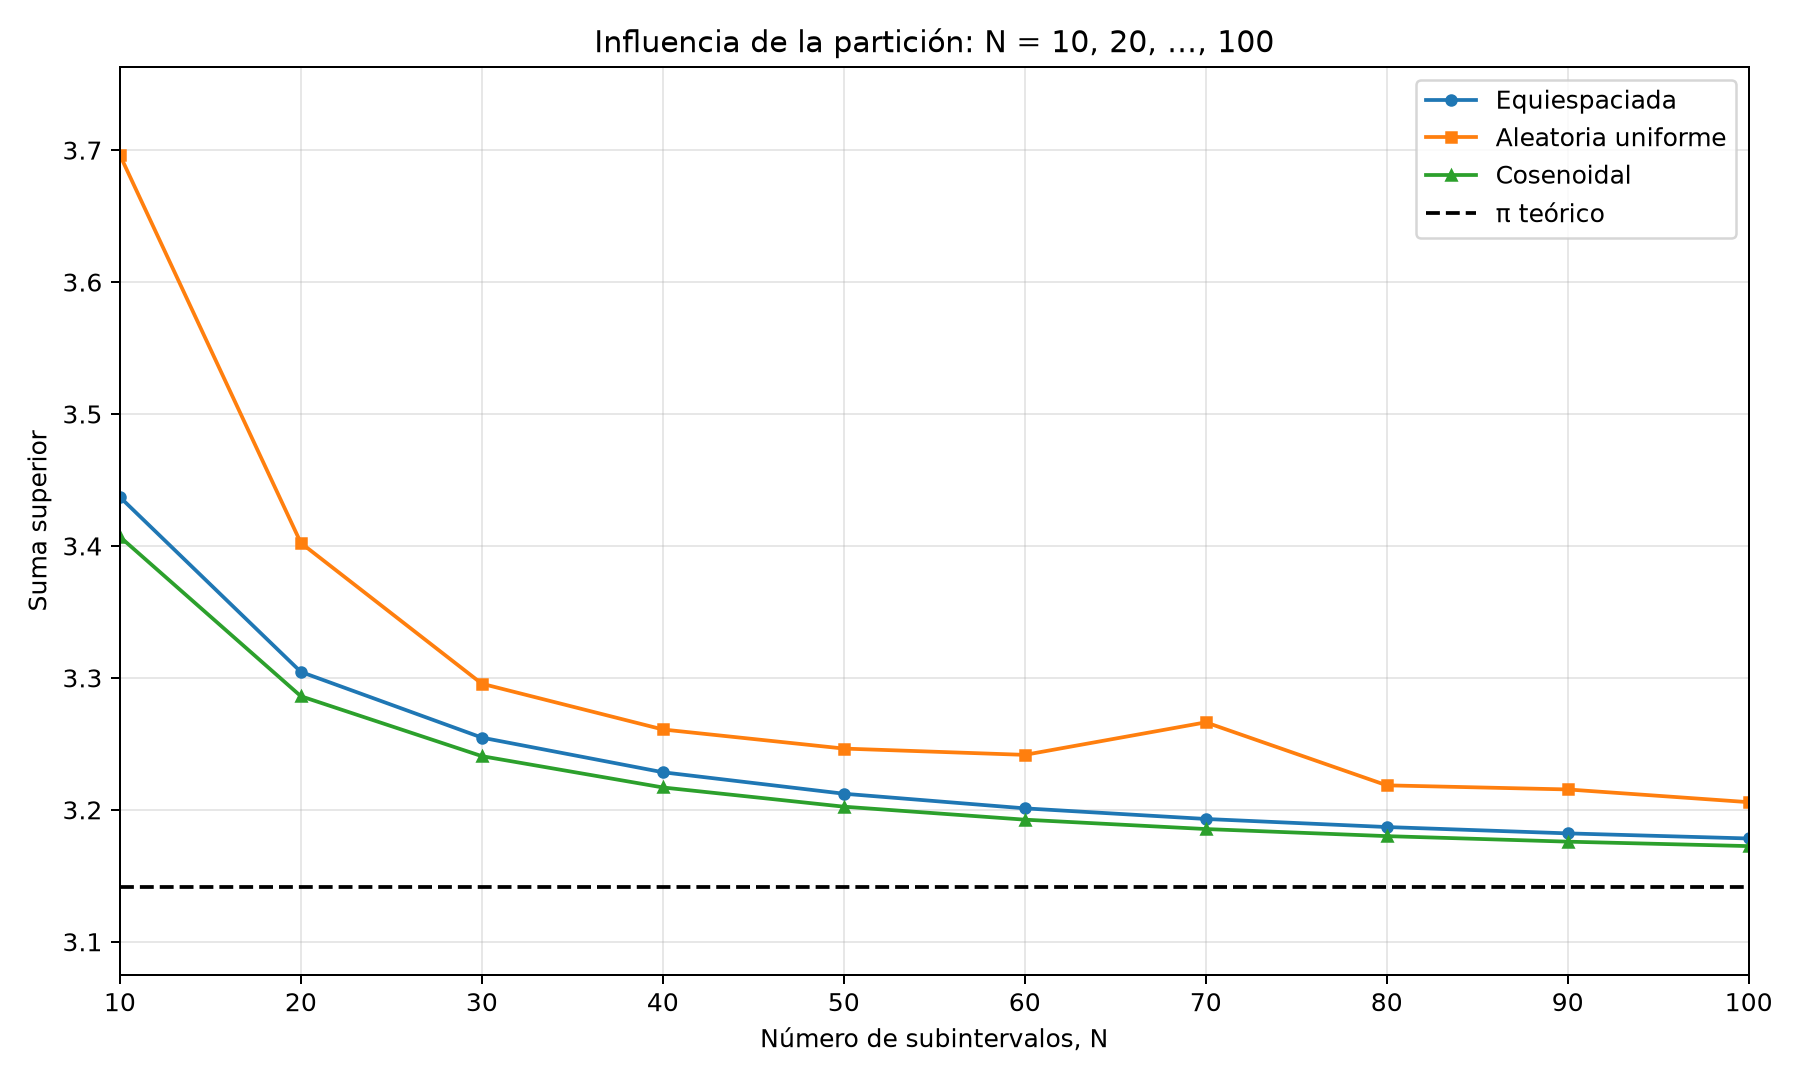
\includegraphics[width=0.88\textwidth]{2grafica_10_a_100.png}
\caption{Suma superior según el tipo de partición para \(N\) entre 10 y 100.}
\label{fig:e2_10a100}
\end{figure}

\begin{figure}[H]
\centering
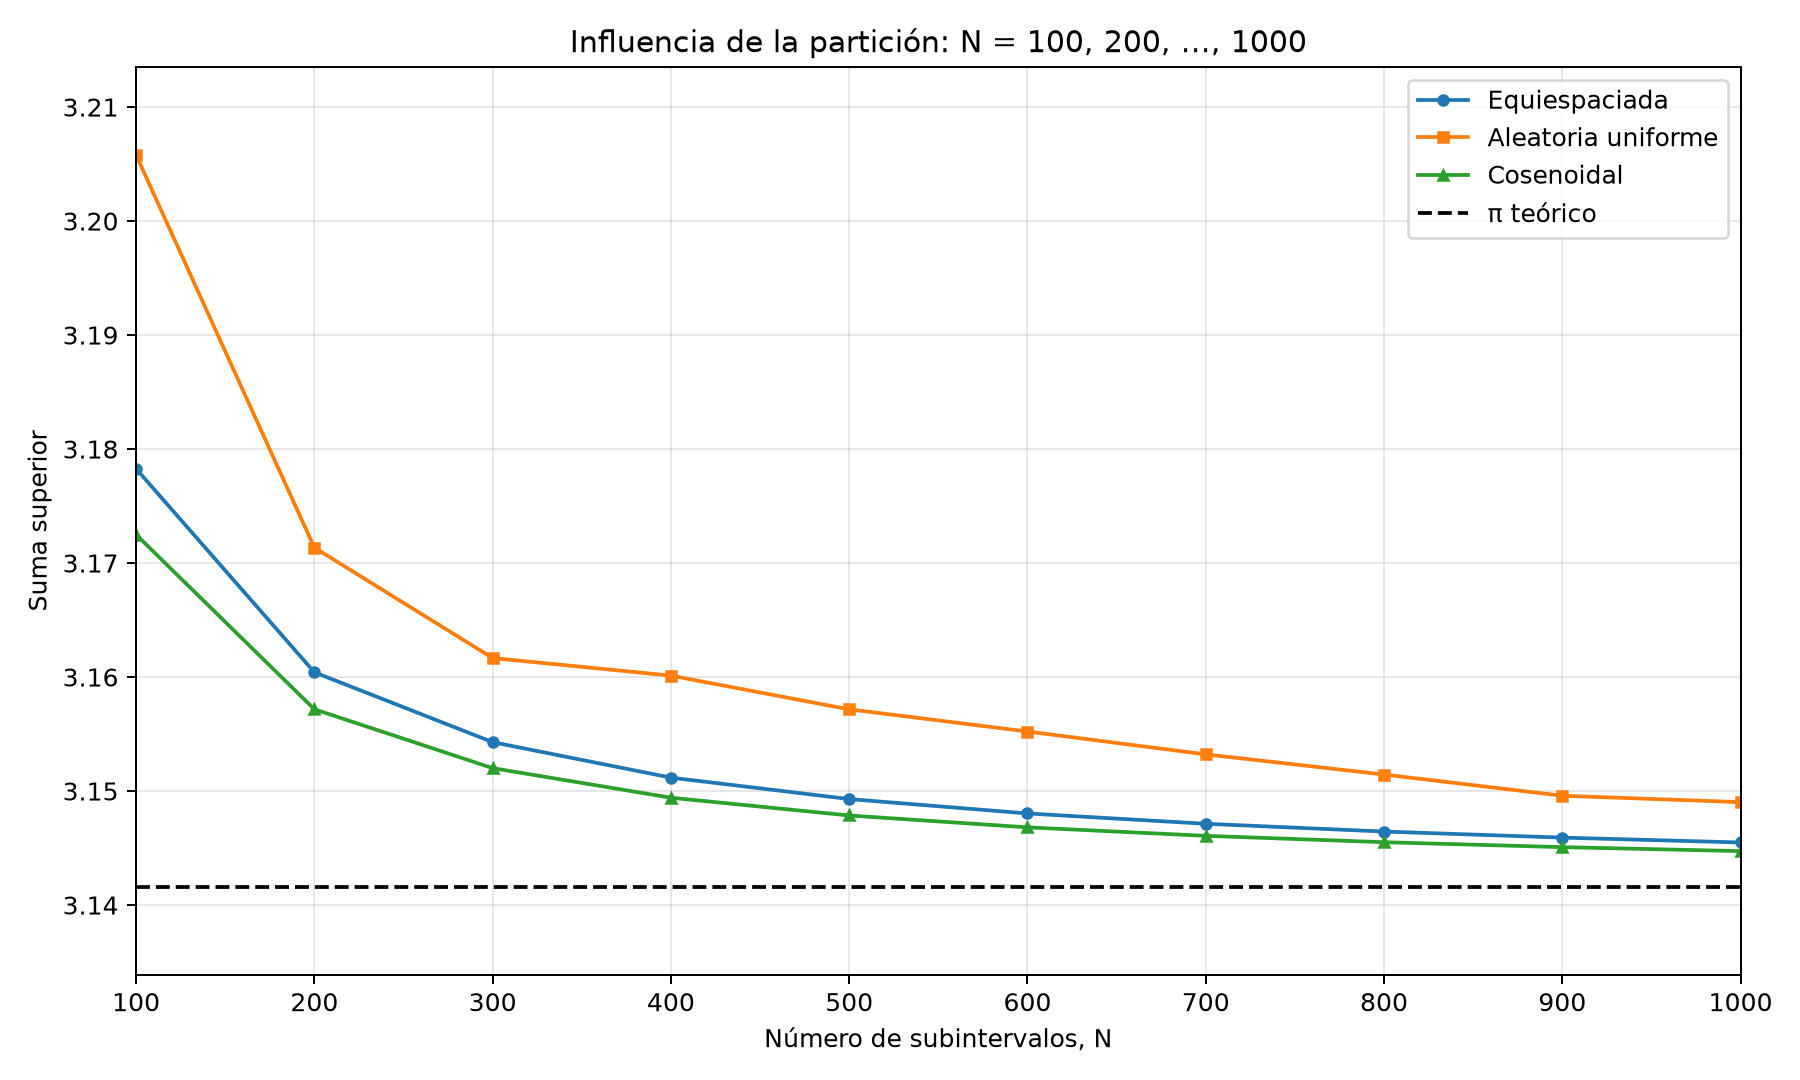
\includegraphics[width=0.88\textwidth]{2grafica_100_a_1000.png}
\caption{Suma superior según el tipo de partición para \(N\) entre 100 y 1000.}
\label{fig:e2_100a1000}
\end{figure}

\begin{figure}[H]
\centering
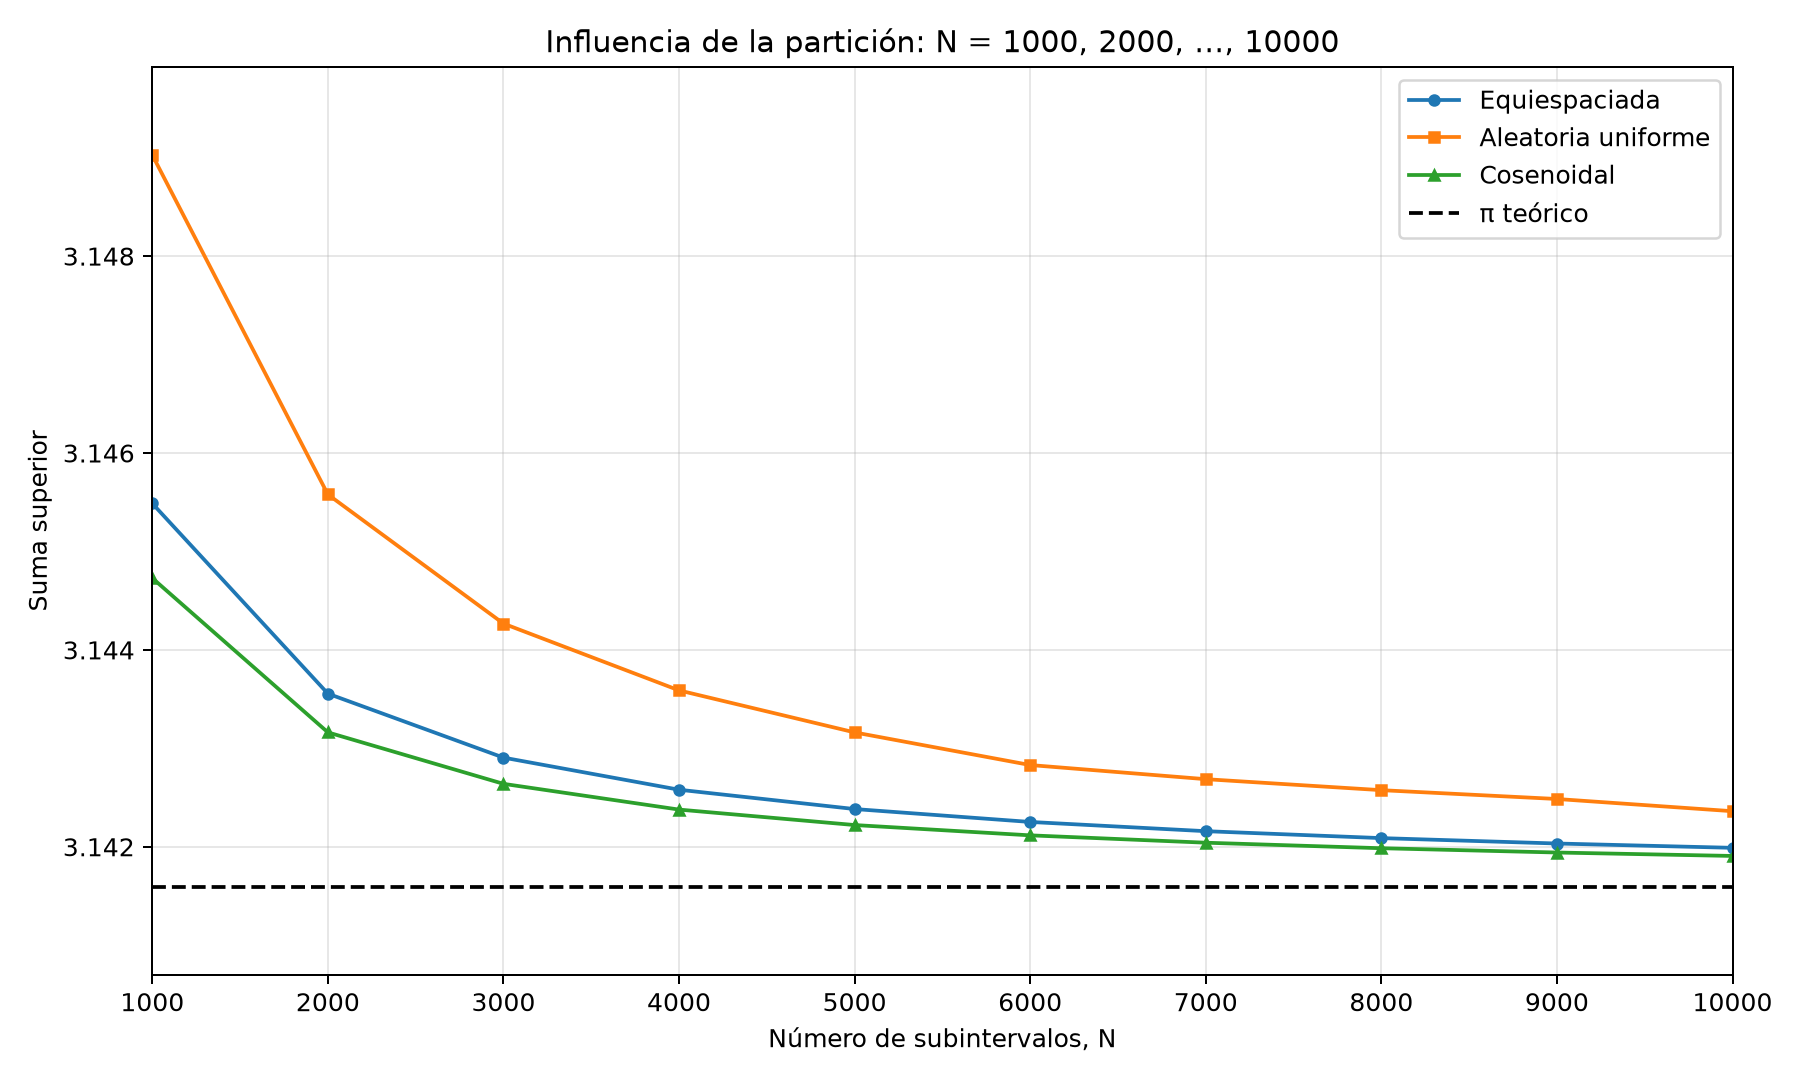
\includegraphics[width=0.88\textwidth]{2grafica_1000_a_10000.png}
\caption{Suma superior según el tipo de partición para \(N\) entre 1000 y 10000.}
\label{fig:e2_1000a10000}
\end{figure}

La consigna también pide graficar la función \(f\) y los rectángulos de la aproximación para cada partición con \(N=100\) (Figura~\ref{fig:e2_rect}). En la equiespaciada todos los rectángulos tienen el mismo ancho; en la aleatoria aparecen rectángulos muy finos junto a otros muy anchos, que sobresalen mucho de la curva; y en la cosenoidal los rectángulos son anchos en el centro y cada vez más finos hacia los bordes.

\begin{figure}[H]
\centering
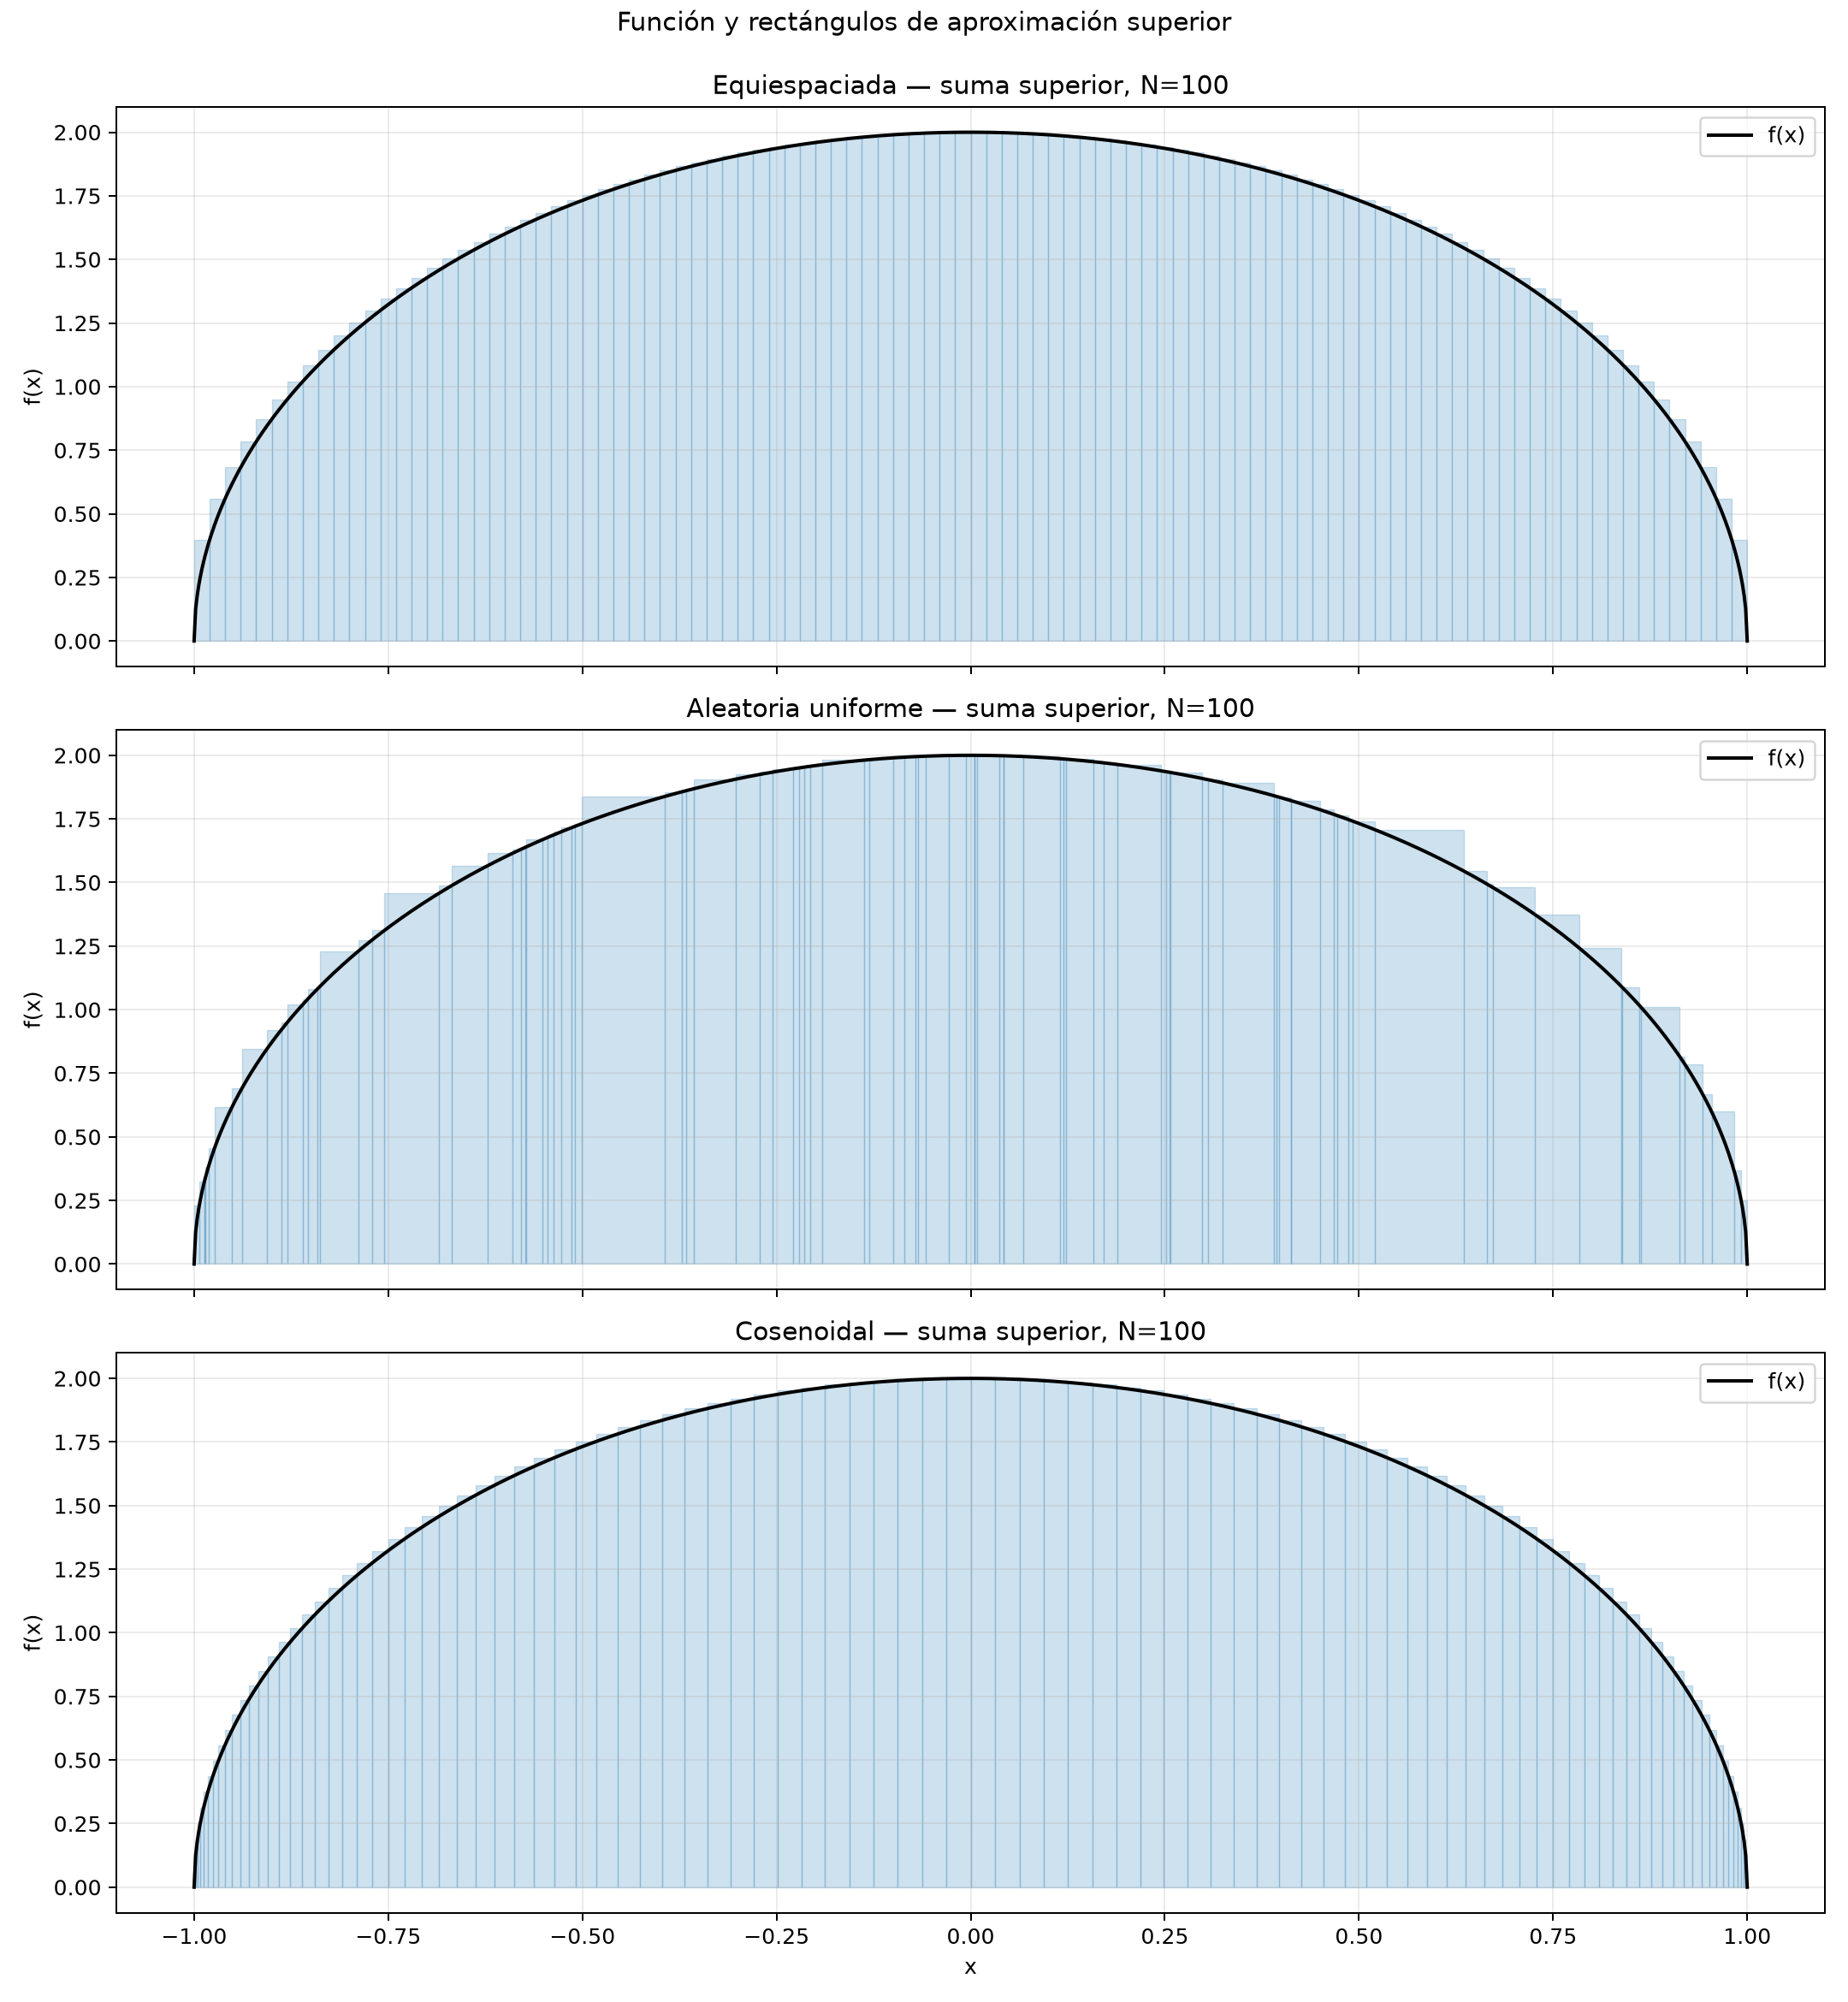
\includegraphics[width=0.85\textwidth]{2rectangulos_N100.png}
\caption{Función \(f\) y rectángulos de la suma superior para cada partición, con \(N=100\).}
\label{fig:e2_rect}
\end{figure}

\subsection{Conclusiones y respuestas analíticas}

\paragraph{¿Qué conclusiones puede tomar? ¿Hay particiones mejores que otras?}
Sí. Las tres particiones convergen a \(\pi\), pero no con la misma precisión: la cosenoidal tiene el menor error en todos los valores de \(N\), seguida por la equiespaciada. La aleatoria uniforme tiene un comportamiento irregular y un error consistentemente mayor (casi el doble que la equiespaciada), porque el azar siempre deja algunos subintervalos desproporcionadamente grandes. Hay que destacar que la mejora de la cosenoidal es moderada: su error es entre un 10\,\% (\(N=10\)) y un 21\,\% (\(N=10000\)) menor que el de la equiespaciada, y en las tres particiones el error disminuye aproximadamente como \(1/N\). Es decir, cambiar la partición reduce el error, pero no cambia la velocidad con la que converge el método.

\paragraph{¿Qué partición dio el mejor resultado? ¿Tiene sentido?}
La partición cosenoidal, \(x_i=\cos\left(\frac{i\pi}{N}\right)\). Tiene sentido: la función \(f(x)=2\sqrt{1-x^2}\) representa una semicircunferencia, cuya pendiente se vuelve vertical en los extremos \(x=\pm1\). En la suma superior, lo que sobra por encima de la curva en cada rectángulo depende de su ancho y de cuánto baja la curva dentro de él. Cerca de los bordes la curva baja muy rápido, así que ahí conviene usar rectángulos finos; en el centro la curva es casi plana y los rectángulos anchos casi no sobresalen. La partición cosenoidal hace exactamente eso: concentra los puntos en los bordes y los separa en el centro.

\paragraph{¿Afecta la geometría de la función a este resultado?}
Sí, la geometría es la explicación. La pendiente vertical en los extremos castiga a las particiones equiespaciada y aleatoria, que dejan subintervalos relativamente grandes justo donde la función cambia más. Los puntos cosenoidales provienen de dividir la circunferencia en ángulos iguales, por lo que se adaptan naturalmente a esta curva. Si la función fuera empinada en el centro y plana en los bordes, juntar los puntos en los extremos no ayudaría: no existe una partición que sea la mejor para todas las funciones, sino que conviene poner más puntos donde la función cambia más rápido.

%=====================================================================
\section{Ejercicio 3: Comparación de métodos}
%=====================================================================

\subsection{Introducción}

En esta sección comparamos tres métodos de integración numérica sobre una misma partición equiespaciada de \([-1,1]\). Como en el Ejercicio 1, \(N\) es la \textbf{cantidad de puntos} de la partición, que forman \(N-1\) subintervalos de ancho
\[
h=\frac{1-(-1)}{N-1}=\frac{2}{N-1},
\qquad x_i=-1+ih,\quad i=0,1,\ldots,N-1.
\]
Los tres métodos son:
\begin{enumerate}
    \item \textbf{Rectángulos (el método usual):} la altura de cada rectángulo es el valor de la función en el extremo izquierdo del subintervalo:
    \[
    R_N=h\sum_{i=0}^{N-2}f(x_i).
    \]
    \item \textbf{Trapecio:} en cada subintervalo se une con una recta los dos puntos de la curva en sus extremos, y se suma el área del trapecio que queda debajo:
    \[
    T_N=\sum_{i=0}^{N-2}\frac{f(x_i)+f(x_{i+1})}{2}\,h.
    \]
    \item \textbf{Punto medio:} la altura de cada rectángulo es el valor de la función en el centro del subintervalo:
    \[
    M_N=h\sum_{i=0}^{N-2}f\!\left(\frac{x_i+x_{i+1}}{2}\right).
    \]
\end{enumerate}
El residuo de cada método se define como \(Q_N-\pi\), donde \(Q_N\) es la aproximación. Un residuo negativo indica que el método subestima la integral y uno positivo, que la sobreestima; para comparar la precisión se mira su valor absoluto.

La Figura~\ref{fig:e3_ilustracion} muestra cómo aproxima el área cada método con solo \(N=6\) puntos.

\begin{figure}[H]
\centering
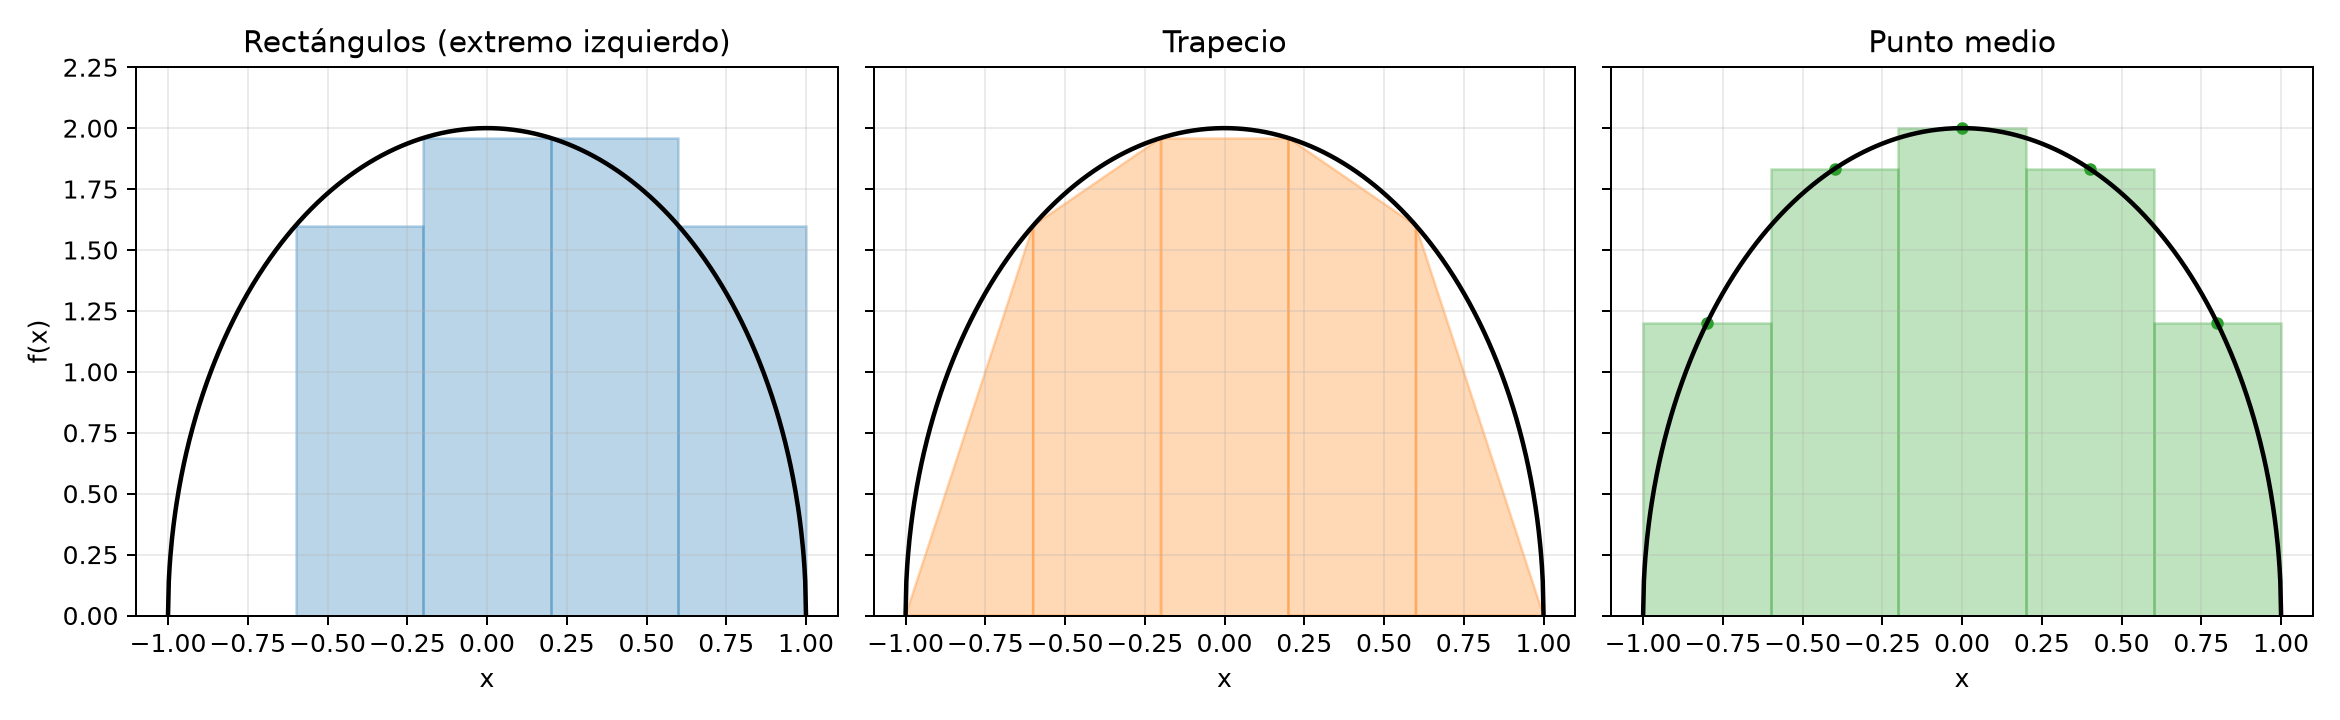
\includegraphics[width=\textwidth]{3metodos_ilustracion.png}
\caption{Aproximación del área con rectángulos (extremo izquierdo), trapecios y punto medio, con \(N=6\) puntos.}
\label{fig:e3_ilustracion}
\end{figure}

\subsection{Implementación en Python}

A continuación se muestra el código implementado en Python para construir la partición y calcular las tres aproximaciones (versión resumida; las funciones que imprimen las tablas, guardan los CSV y dibujan las gráficas se omiten):

\begin{lstlisting}[language=Python, caption={Código fuente del Ejercicio 3 (versión resumida)}]
import math

A = -1.0
B = 1.0
PI = math.pi

RANGOS_N = {
    "10_a_100": range(10, 101, 10),
    "100_a_1000": range(100, 1001, 100),
    "1000_a_10000": range(1000, 10001, 1000),
}

def f(x: float) -> float:
    return 2.0 * math.sqrt(max(0.0, 1.0 - x * x))

def particion_equiespaciada(n: int) -> list[float]:
    """N puntos equiespaciados, incluyendo -1 y 1 (N-1 subintervalos)."""
    if not isinstance(n, int) or isinstance(n, bool) or n < 2:
        raise ValueError("N debe ser un entero de al menos 2 puntos")
    return [A + (B - A) * i / (n - 1) for i in range(n)]

def metodo_rectangulos(puntos: list[float]) -> float:
    suma = 0.0
    for x_izq, x_der in zip(puntos, puntos[1:]):
        suma += f(x_izq) * (x_der - x_izq)
    return suma

def metodo_trapecio(puntos: list[float]) -> float:
    suma = 0.0
    for x_izq, x_der in zip(puntos, puntos[1:]):
        suma += (f(x_izq) + f(x_der)) * (x_der - x_izq) / 2.0
    return suma

def metodo_punto_medio(puntos: list[float]) -> float:
    suma = 0.0
    for x_izq, x_der in zip(puntos, puntos[1:]):
        punto_medio = (x_izq + x_der) / 2.0
        suma += f(punto_medio) * (x_der - x_izq)
    return suma

def generar_registros(valores_n: list[int]) -> list[dict[str, float | int]]:
    metodos = {
        "rectangulos": metodo_rectangulos,
        "trapecio": metodo_trapecio,
        "punto_medio": metodo_punto_medio,
    }
    registros = []
    for n in valores_n:
        puntos = particion_equiespaciada(n)
        registro: dict[str, float | int] = {"N": n}
        for nombre, funcion_metodo in metodos.items():
            aprox = funcion_metodo(puntos)
            registro[f"aprox_{nombre}"] = aprox
            registro[f"residuo_{nombre}"] = aprox - PI
        registros.append(registro)
    return registros
\end{lstlisting}

\subsection{Tablas comparativas de resultados}

Las siguientes tablas muestran la aproximación de cada método y su residuo. Como los residuos se hacen muy chicos, se escriben en notación científica.

\begin{table}[H]
\centering
\caption{Aproximación según el método, \(N\) entre 10 y 100, en incrementos de 10.}
\label{tab:e3_10a100}
\footnotesize
\setlength{\tabcolsep}{3pt}
\begin{tabular}{r r r r r r r}
\toprule
\(N\) & Rectángulos & Residuo & Trapecio & Residuo & Punto medio & Residuo \\
\midrule
10    & 3.01923183 & \(-1.2236\times10^{-1}\) & 3.01923183 & \(-1.2236\times10^{-1}\) & 3.17713893 & \(+3.5546\times10^{-2}\) \\
20    & 3.10155965 & \(-4.0033\times10^{-2}\) & 3.10155965 & \(-4.0033\times10^{-2}\) & 3.15327255 & \(+1.1680\times10^{-2}\) \\
30    & 3.12033906 & \(-2.1254\times10^{-2}\) & 3.12033906 & \(-2.1254\times10^{-2}\) & 3.14780184 & \(+6.2092\times10^{-3}\) \\
40    & 3.12795728 & \(-1.3635\times10^{-2}\) & 3.12795728 & \(-1.3635\times10^{-2}\) & 3.14557880 & \(+3.9861\times10^{-3}\) \\
50    & 3.13190745 & \(-9.6852\times10^{-3}\) & 3.13190745 & \(-9.6852\times10^{-3}\) & 3.14442511 & \(+2.8325\times10^{-3}\) \\
60    & 3.13426075 & \(-7.3319\times10^{-3}\) & 3.13426075 & \(-7.3319\times10^{-3}\) & 3.14373743 & \(+2.1448\times10^{-3}\) \\
70    & 3.13579454 & \(-5.7981\times10^{-3}\) & 3.13579454 & \(-5.7981\times10^{-3}\) & 3.14328906 & \(+1.6964\times10^{-3}\) \\
80    & 3.13685931 & \(-4.7333\times10^{-3}\) & 3.13685931 & \(-4.7333\times10^{-3}\) & 3.14297772 & \(+1.3851\times10^{-3}\) \\
90    & 3.13763387 & \(-3.9588\times10^{-3}\) & 3.13763387 & \(-3.9588\times10^{-3}\) & 3.14275119 & \(+1.1585\times10^{-3}\) \\
100   & 3.13821804 & \(-3.3746\times10^{-3}\) & 3.13821804 & \(-3.3746\times10^{-3}\) & 3.14258032 & \(+9.8766\times10^{-4}\) \\
\bottomrule
\end{tabular}
\end{table}

\begin{table}[H]
\centering
\caption{Aproximación según el método, \(N\) entre 100 y 1000, en incrementos de 100.}
\label{tab:e3_100a1000}
\footnotesize
\setlength{\tabcolsep}{3pt}
\begin{tabular}{r r r r r r r}
\toprule
\(N\) & Rectángulos & Residuo & Trapecio & Residuo & Punto medio & Residuo \\
\midrule
100   & 3.13821804 & \(-3.3746\times10^{-3}\) & 3.13821804 & \(-3.3746\times10^{-3}\) & 3.14258032 & \(+9.8766\times10^{-4}\) \\
200   & 3.14040816 & \(-1.1845\times10^{-3}\) & 3.14040816 & \(-1.1845\times10^{-3}\) & 3.14193945 & \(+3.4680\times10^{-4}\) \\
300   & 3.14094945 & \(-6.4321\times10^{-4}\) & 3.14094945 & \(-6.4321\times10^{-4}\) & 3.14178100 & \(+1.8834\times10^{-4}\) \\
400   & 3.14117538 & \(-4.1727\times10^{-4}\) & 3.14117538 & \(-4.1727\times10^{-4}\) & 3.14171485 & \(+1.2219\times10^{-4}\) \\
500   & 3.14129429 & \(-2.9836\times10^{-4}\) & 3.14129429 & \(-2.9836\times10^{-4}\) & 3.14168003 & \(+8.7375\times10^{-5}\) \\
600   & 3.14136579 & \(-2.2686\times10^{-4}\) & 3.14136579 & \(-2.2686\times10^{-4}\) & 3.14165909 & \(+6.6438\times10^{-5}\) \\
700   & 3.14141269 & \(-1.7997\times10^{-4}\) & 3.14141269 & \(-1.7997\times10^{-4}\) & 3.14164536 & \(+5.2705\times10^{-5}\) \\
800   & 3.14144539 & \(-1.4726\times10^{-4}\) & 3.14144539 & \(-1.4726\times10^{-4}\) & 3.14163578 & \(+4.3128\times10^{-5}\) \\
900   & 3.14146926 & \(-1.2339\times10^{-4}\) & 3.14146926 & \(-1.2339\times10^{-4}\) & 3.14162879 & \(+3.6137\times10^{-5}\) \\
1000  & 3.14148732 & \(-1.0533\times10^{-4}\) & 3.14148732 & \(-1.0533\times10^{-4}\) & 3.14162350 & \(+3.0849\times10^{-5}\) \\
\bottomrule
\end{tabular}
\end{table}

\begin{table}[H]
\centering
\caption{Aproximación según el método, \(N\) entre 1000 y 10000, en incrementos de 1000.}
\label{tab:e3_1000a10000}
\footnotesize
\setlength{\tabcolsep}{3pt}
\begin{tabular}{r r r r r r r}
\toprule
\(N\) & Rectángulos & Residuo & Trapecio & Residuo & Punto medio & Residuo \\
\midrule
1000  & 3.14148732 & \(-1.0533\times10^{-4}\) & 3.14148732 & \(-1.0533\times10^{-4}\) & 3.14162350 & \(+3.0849\times10^{-5}\) \\
2000  & 3.14155544 & \(-3.7215\times10^{-5}\) & 3.14155544 & \(-3.7215\times10^{-5}\) & 3.14160355 & \(+1.0899\times10^{-5}\) \\
3000  & 3.14157240 & \(-2.0252\times10^{-5}\) & 3.14157240 & \(-2.0252\times10^{-5}\) & 3.14159859 & \(+5.9316\times10^{-6}\) \\
4000  & 3.14157950 & \(-1.3153\times10^{-5}\) & 3.14157950 & \(-1.3153\times10^{-5}\) & 3.14159651 & \(+3.8522\times10^{-6}\) \\
5000  & 3.14158324 & \(-9.4106\times10^{-6}\) & 3.14158324 & \(-9.4106\times10^{-6}\) & 3.14159541 & \(+2.7562\times10^{-6}\) \\
6000  & 3.14158550 & \(-7.1585\times10^{-6}\) & 3.14158550 & \(-7.1585\times10^{-6}\) & 3.14159475 & \(+2.0967\times10^{-6}\) \\
7000  & 3.14158697 & \(-5.6805\times10^{-6}\) & 3.14158697 & \(-5.6805\times10^{-6}\) & 3.14159432 & \(+1.6638\times10^{-6}\) \\
8000  & 3.14158800 & \(-4.6493\times10^{-6}\) & 3.14158800 & \(-4.6493\times10^{-6}\) & 3.14159402 & \(+1.3617\times10^{-6}\) \\
9000  & 3.14158876 & \(-3.8963\times10^{-6}\) & 3.14158876 & \(-3.8963\times10^{-6}\) & 3.14159379 & \(+1.1412\times10^{-6}\) \\
10000 & 3.14158933 & \(-3.3267\times10^{-6}\) & 3.14158933 & \(-3.3267\times10^{-6}\) & 3.14159363 & \(+9.7435\times10^{-7}\) \\
\bottomrule
\end{tabular}
\end{table}

Lo primero que llama la atención es que \textbf{rectángulos y trapecio dan exactamente el mismo resultado} en todas las filas. No es un error del programa: como \(f(-1)=f(1)=0\), el primer rectángulo tiene altura cero, y en la fórmula del trapecio los dos extremos también aportan cero, así que las dos fórmulas terminan sumando exactamente los mismos términos:
\[
R_N=h\sum_{i=1}^{N-2}f(x_i)=T_N.
\]
Además, rectángulos y trapecio siempre quedan por debajo de \(\pi\) (residuo negativo), mientras que el punto medio siempre queda por encima (residuo positivo) y con un error absoluto unas tres veces menor.

\subsection{Análisis de las gráficas}

Las gráficas muestran las tres aproximaciones junto con el valor exacto \(\pi\) para cada rango de \(N\). Las curvas de rectángulos y trapecio aparecen superpuestas porque sus valores coinciden.

\begin{figure}[H]
\centering
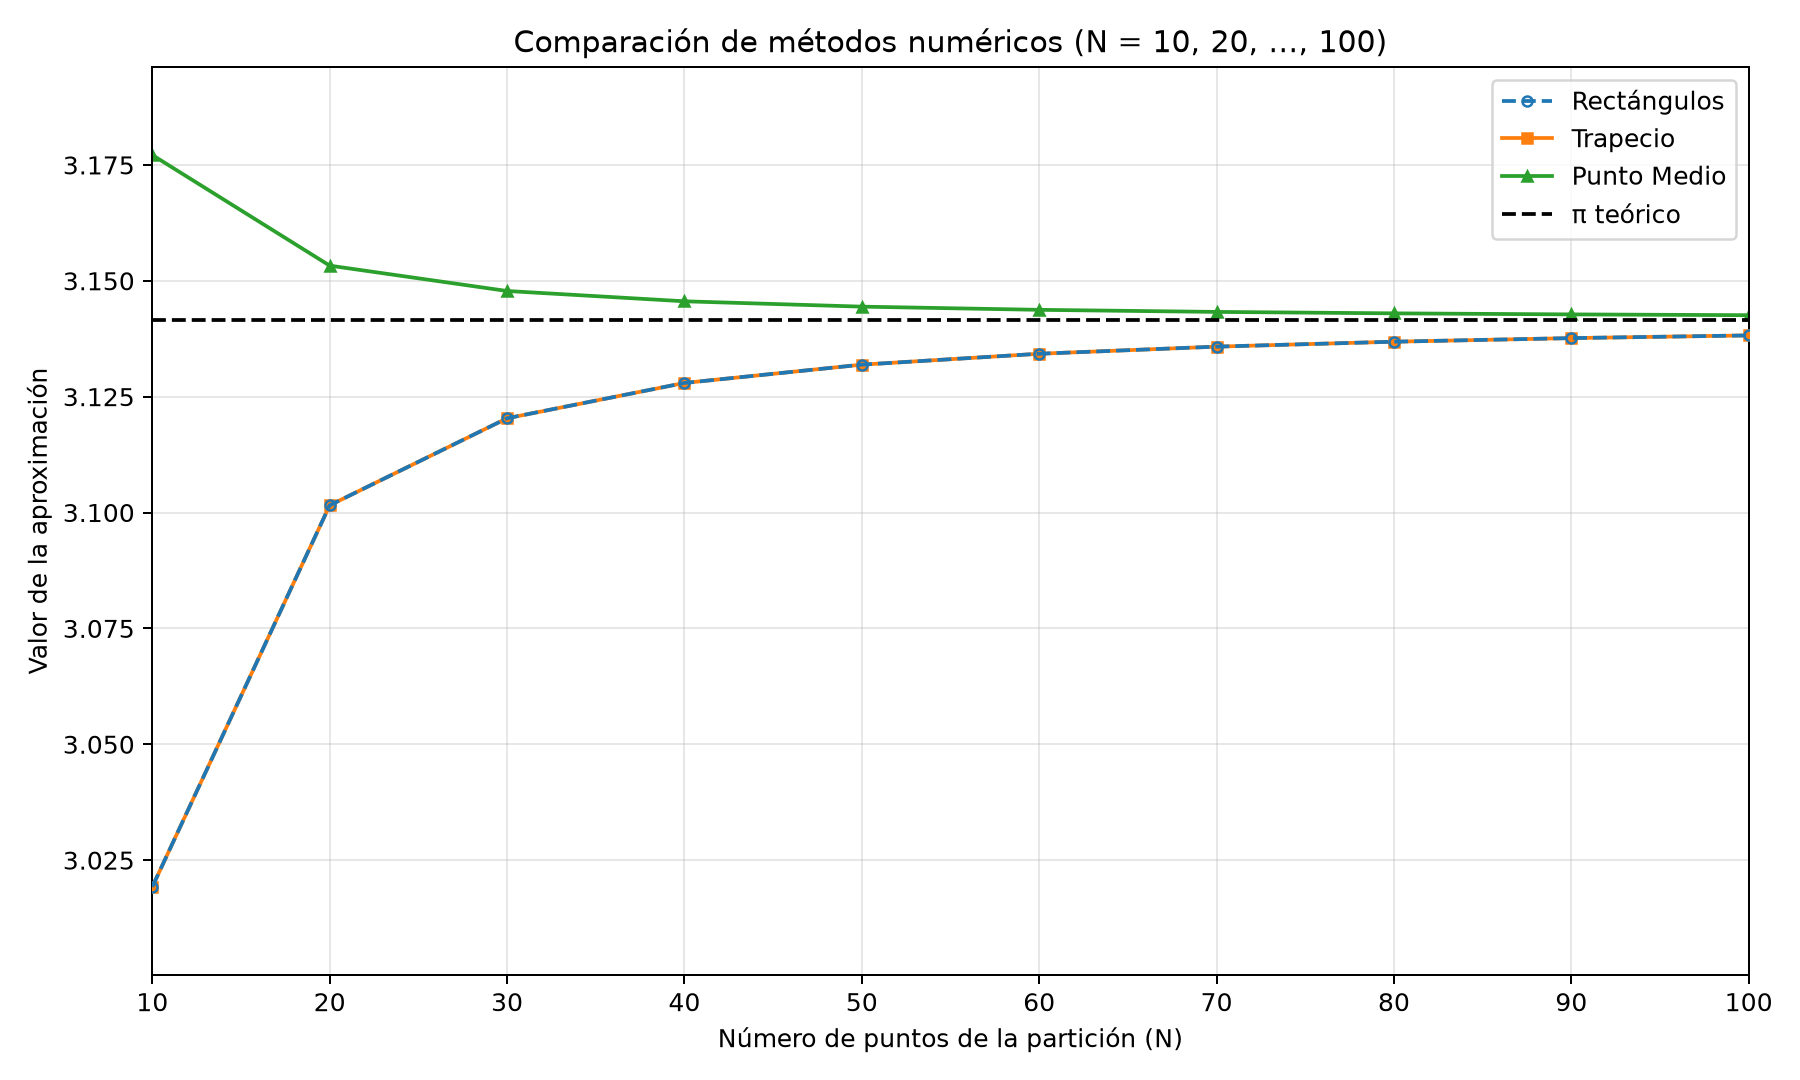
\includegraphics[width=0.88\textwidth]{3grafica_metodos_10_a_100.png}
\caption{Aproximación según el método para \(N\) entre 10 y 100.}
\label{fig:e3_10a100}
\end{figure}

\begin{figure}[H]
\centering
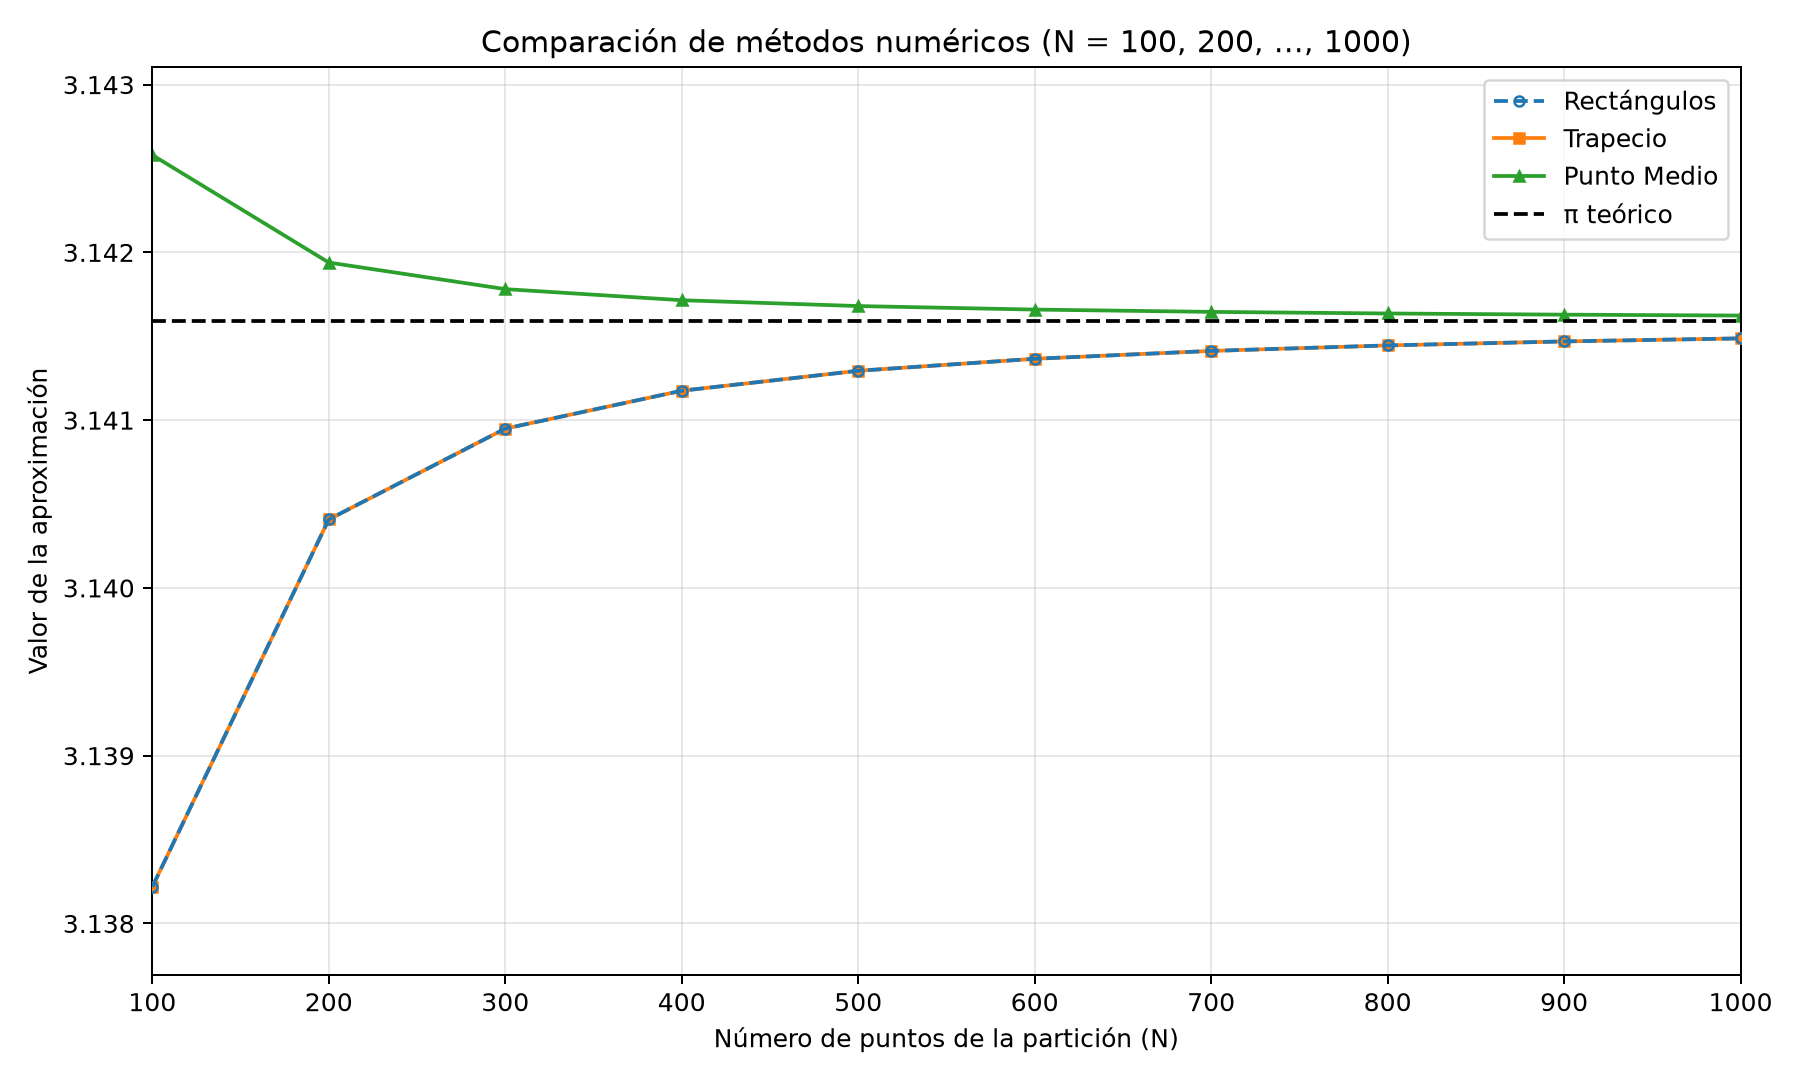
\includegraphics[width=0.88\textwidth]{3grafica_metodos_100_a_1000.png}
\caption{Aproximación según el método para \(N\) entre 100 y 1000.}
\label{fig:e3_100a1000}
\end{figure}

\begin{figure}[H]
\centering
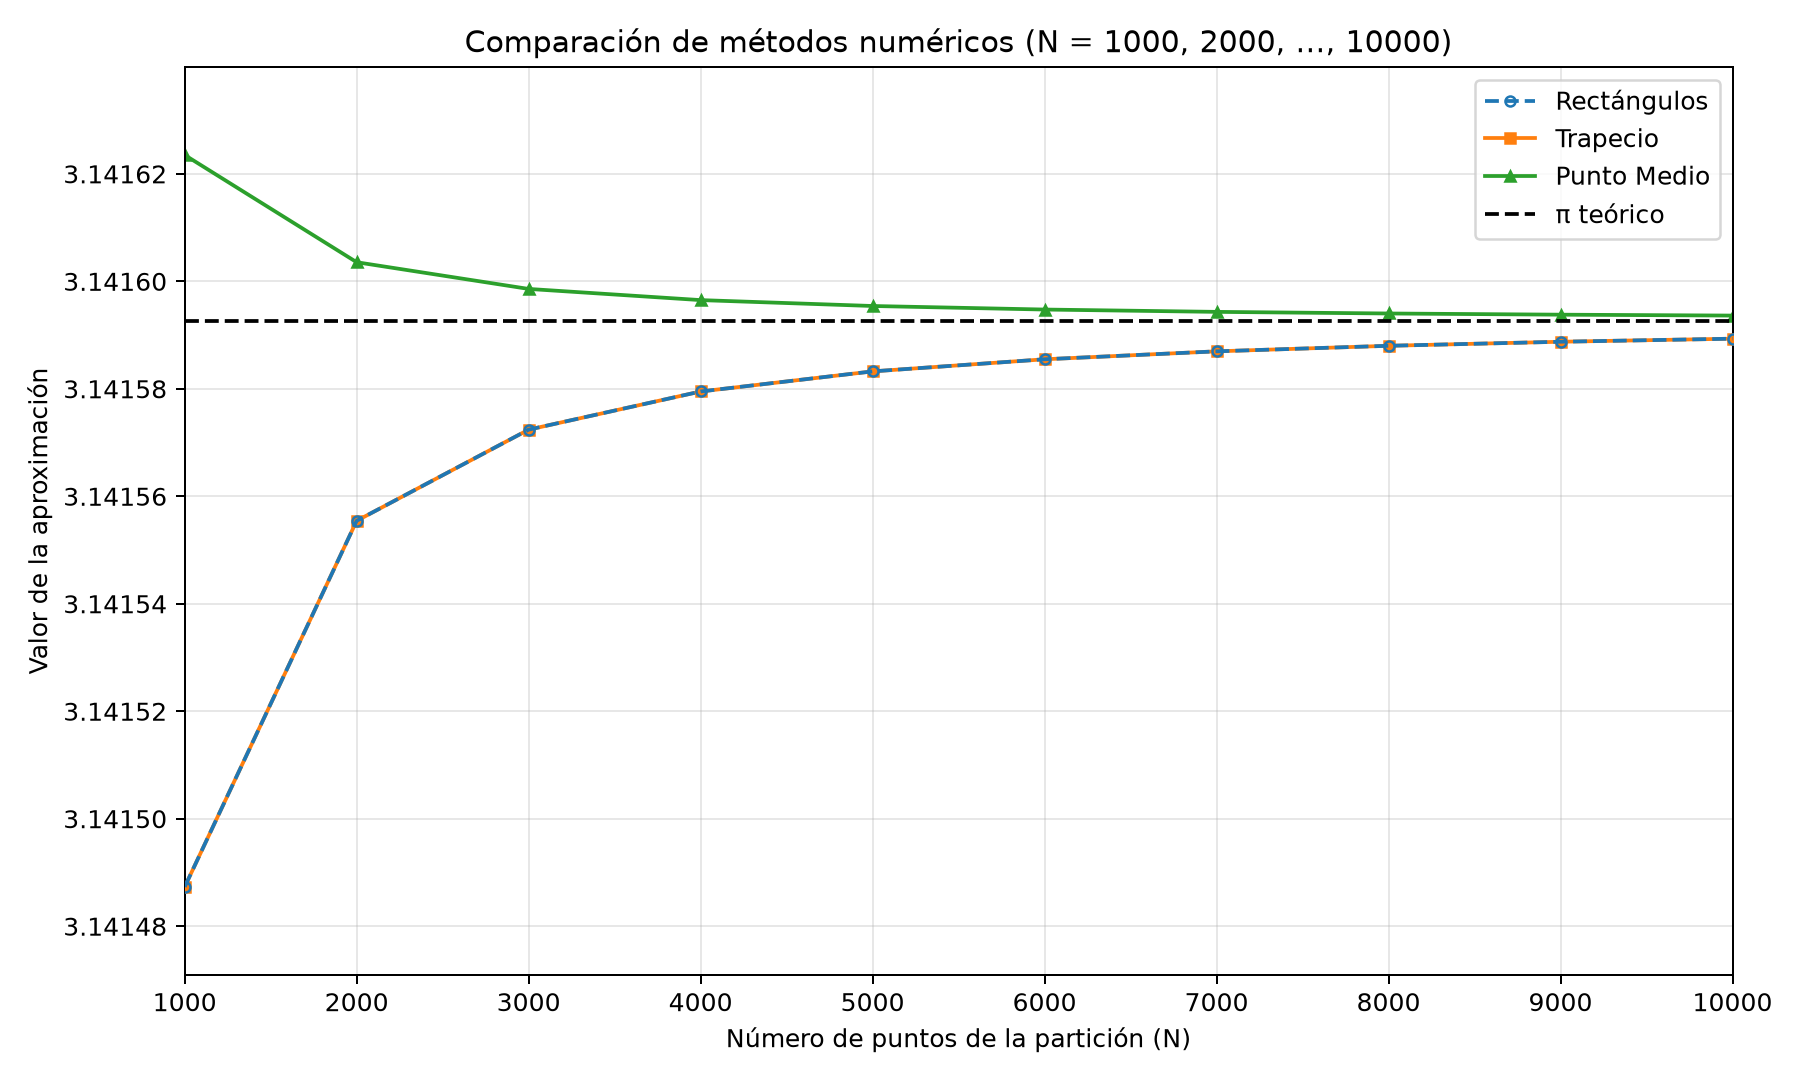
\includegraphics[width=0.88\textwidth]{3grafica_metodos_1000_a_10000.png}
\caption{Aproximación según el método para \(N\) entre 1000 y 10000.}
\label{fig:e3_1000a10000}
\end{figure}

Para ver mejor qué tan rápido baja el error, la Figura~\ref{fig:e3_log} muestra el valor absoluto del residuo en escala logarítmica (cada marca de los ejes representa multiplicar por 10).

\begin{figure}[H]
\centering
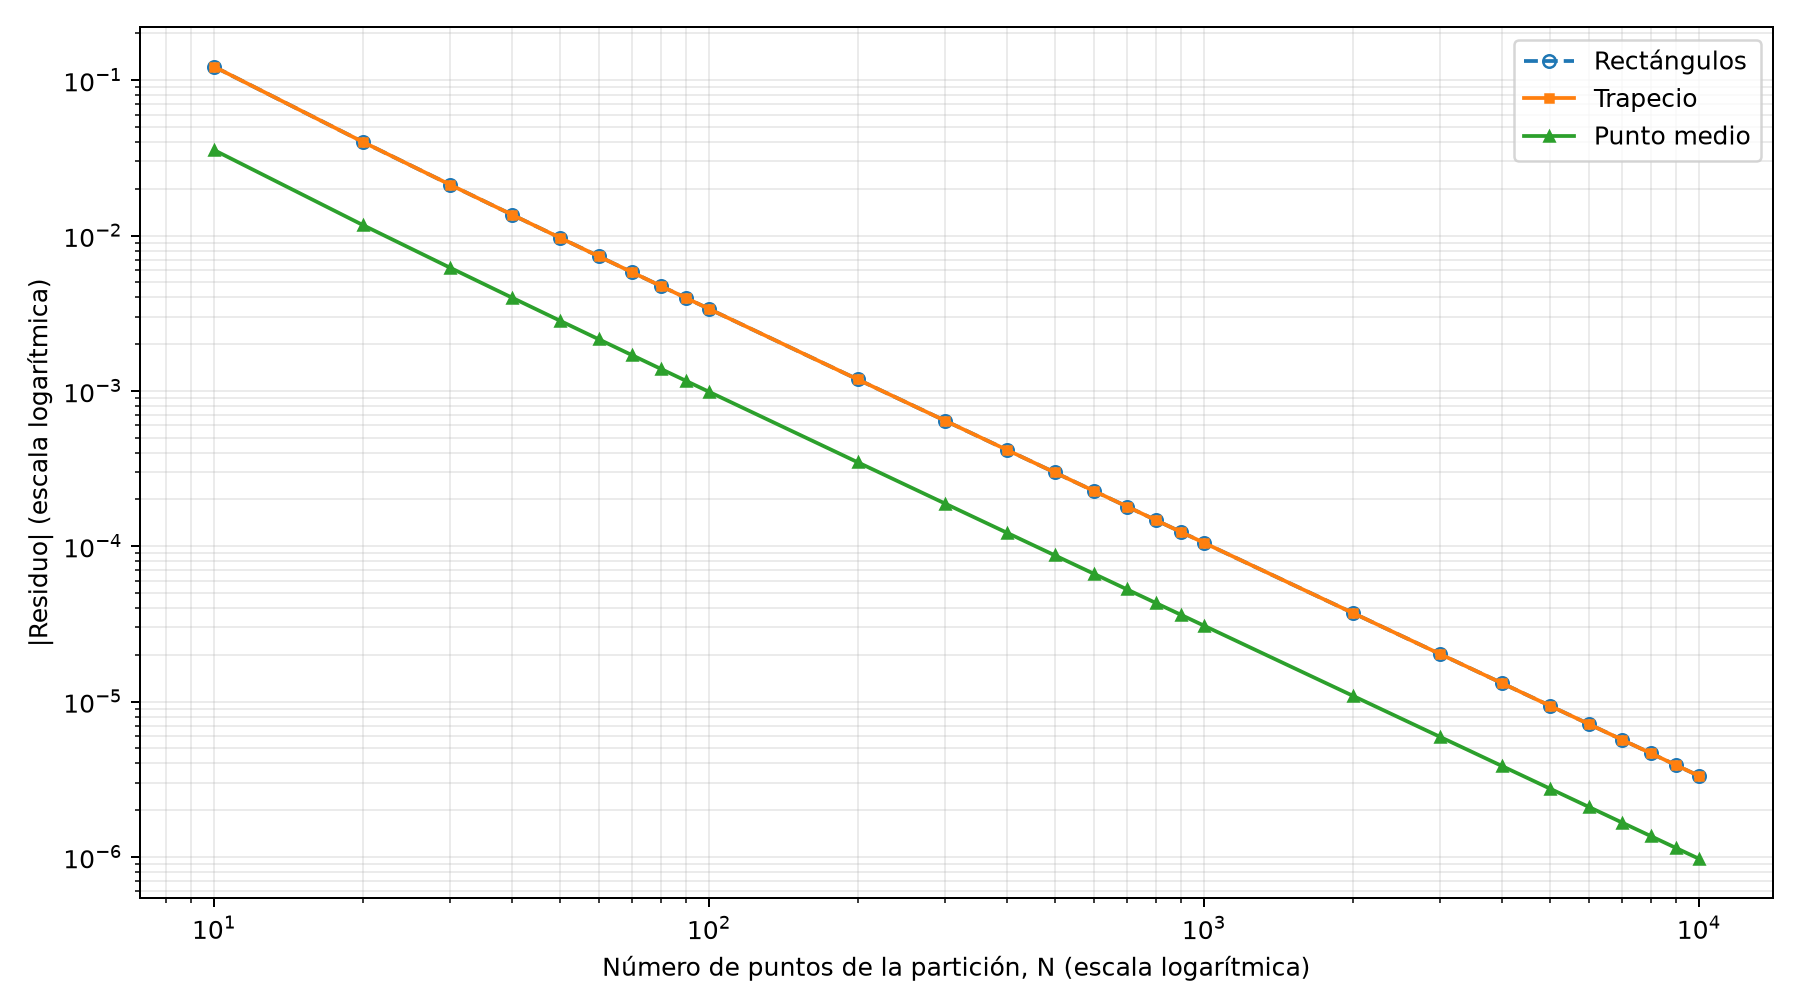
\includegraphics[width=0.88\textwidth]{3errores_log.png}
\caption{Valor absoluto del residuo de cada método según \(N\), en escala logarítmica.}
\label{fig:e3_log}
\end{figure}

Las tres líneas son rectas y paralelas: cada vez que \(N\) se multiplica por 10, el error se divide aproximadamente por 32 (por ejemplo, el residuo del trapecio pasa de \(3.37\times10^{-3}\) con \(N=100\) a \(1.05\times10^{-4}\) con \(N=1000\)). Esto es mucho mejor que las sumas de Darboux de los Ejercicios 1 y 2, donde el error solo se dividía por 10. Con \(N=10000\), el trapecio tiene un error de \(3.3\times10^{-6}\), unas 100 veces menor que el de la suma superior con la misma partición (\(4.0\times10^{-4}\)).

\subsection{Conclusiones y respuestas analíticas}

\paragraph{¿Qué método dio mejores resultados?}
El \textbf{punto medio}. En todos los valores de \(N\) su residuo es el más chico en valor absoluto: aproximadamente un 29\,\% del error del trapecio (por ejemplo, \(9.88\times10^{-4}\) contra \(3.37\times10^{-3}\) con \(N=100\)). Rectángulos y trapecio quedan empatados, porque en este problema dan exactamente el mismo resultado.

\paragraph{¿Hay métodos mejores que otros?}
Sí, pero hay que matizarlo. En general, el trapecio es mejor que los rectángulos, porque reemplaza la ``escalera'' de rectángulos por segmentos que siguen la inclinación de la curva. En este ejercicio esa ventaja no se ve, porque la función vale cero en los dos extremos del intervalo y las dos fórmulas coinciden. Si la función no se anulara en los extremos, los resultados serían distintos. El punto medio, en cambio, sí resulta mejor que los otros dos para esta función.

\paragraph{Justificación geométrica.}
La clave es que la función es \textbf{cóncava hacia abajo} (tiene forma de cúpula):
\[
f''(x)=-\frac{2}{(1-x^2)^{3/2}}<0,\qquad -1<x<1.
\]
\begin{itemize}
    \item \textbf{Trapecio:} el lado de arriba de cada trapecio es una cuerda que une dos puntos de la curva. En una curva cóncava hacia abajo, las cuerdas quedan siempre \textbf{por debajo} de la curva, así que cada trapecio deja un pequeño hueco sin cubrir y la suma total queda por debajo de \(\pi\) (Figura~\ref{fig:e3_ilustracion}, centro).
    \item \textbf{Punto medio:} el área del rectángulo de punto medio es igual al área del trapecio que se forma con la \textbf{recta tangente} a la curva en el centro del subintervalo (lo que el rectángulo agrega de un lado de la tangente lo quita del otro). En una curva cóncava hacia abajo, la tangente queda \textbf{por encima} de la curva, así que el punto medio sobreestima la integral y su residuo es positivo.
    \item \textbf{¿Por qué el punto medio se equivoca menos?} Cerca del centro del subintervalo, la tangente se ``pega'' a la curva mucho más que la cuerda, que solo la toca en los extremos. Por eso el espacio entre la tangente y la curva es más chico que el espacio entre la cuerda y la curva. En funciones suaves el error del punto medio suele ser la mitad del error del trapecio; en nuestra función resultó todavía menor (alrededor del 29\,\%).
\end{itemize}

Por último, el error de los tres métodos baja a un ritmo de aproximadamente \(N^{-1.5}\) (dividido por 32 cada vez que \(N\) se multiplica por 10), y no como \(N^{-2}\), que es lo habitual para el trapecio y el punto medio. Esto también se explica por la geometría: en los extremos \(x=\pm1\) la curva cae en vertical, y ahí ninguna recta (ni la cuerda ni la tangente) la puede seguir bien, así que la mayor parte del error se concentra en los subintervalos de los bordes.

%=====================================================================
\section{Conclusiones generales}
%=====================================================================

En los tres ejercicios aproximamos \(\pi\) como el área bajo \(f(x)=2\sqrt{1-x^2}\), y todos los métodos convergieron al valor exacto al aumentar \(N\), como corresponde a una función continua e integrable de Riemann. Sin embargo, no todas las estrategias mejoran igual. Cambiar la forma de la partición (Ejercicio 2) redujo el error de la suma superior entre un 10\,\% y un 21\,\%, pero mantuvo el mismo ritmo de convergencia que en el Ejercicio 1, donde el error se dividía por 10 cada vez que \(N\) se multiplicaba por 10. En cambio, cambiar la forma de calcular el área de cada subintervalo (Ejercicio 3) cambió el ritmo: con trapecio y punto medio el error se dividió por 32, y el punto medio fue el método más preciso de todos los que probamos.

%=====================================================================
\section*{Referencias}
\addcontentsline{toc}{section}{Referencias}
%=====================================================================

\begingroup
\setlength{\parindent}{-1.27cm}
\setlength{\leftskip}{1.27cm}
\setlength{\parskip}{6pt}

Hunter, J. D. (2007). Matplotlib: A 2D graphics environment. \textit{Computing in Science \& Engineering, 9}(3), 90--95. \url{https://doi.org/10.1109/MCSE.2007.55}

Python Software Foundation. (s.f.). \textit{Python} [Software]. \url{https://www.python.org}

Stewart, J. (2012). \textit{Cálculo de una variable: Trascendentes tempranas} (7.ª ed.; M. C. Rodríguez Pedroza, Trad.). Cengage Learning.

Universidad Católica del Uruguay. (2026). \textit{Comparación de métodos de integración numérica} [Consigna del proyecto grupal, Cálculo Aplicado]. Facultad de Ingeniería y Tecnología.

\endgroup

%=====================================================================

% Los bloques de código se llaman "Código 1, 2, 3" en lugar de "Listing"
\renewcommand{\lstlistingname}{Código}

%=====================================================================
\section{Ejercicio 1: Convergencia de las sumas inferior y superior}
%=====================================================================

\subsection{Introducción y análisis teórico}

La función y el intervalo bajo estudio son:
\[
f(x)=2\sqrt{1-x^2}, \qquad x\in[-1,1].
\]

La ecuación \(x^2+y^2=1\) describe el círculo unitario. Su semicircunferencia superior corresponde a \(y=\sqrt{1-x^2}\). La función del ejercicio es el doble de dicha altura, es decir, \(f(x)=2y\). El área de la semicircunferencia unitaria es \(\pi/2\); al duplicar las alturas, el área exacta bajo la curva es:
\[
\int_{-1}^{1}2\sqrt{1-x^2}\,dx=\pi.
\]

\subsection{Cómo se forman las sumas}

Para un valor de \(N\), se consideran \(N\) puntos equiespaciados, que generan \(N-1\) subintervalos de igual ancho:
\[
\Delta x=\frac{1-(-1)}{N-1}=\frac{2}{N-1}.
\]
Los puntos de la partición son \(x_i=-1+i\Delta x\), para \(i=0,1,\ldots,N-1\). Si \(m_i\) y \(M_i\) son, respectivamente, el mínimo y el máximo de la función en cada subintervalo, las sumas de Darboux son:
\[
L_N=\sum_{i=1}^{N-1}m_i\Delta x,\qquad
U_N=\sum_{i=1}^{N-1}M_i\Delta x.
\]

Como la función es simétrica respecto del eje \(y\), su valor aumenta desde los extremos hasta alcanzar \(2\) en \(x=0\), y luego disminuye. Por eso, en cada subintervalo, el máximo corresponde al punto más cercano a cero y el mínimo al extremo con mayor valor absoluto.

\subsection{Implementación en Python}

El programa, escrito en Python (Python Software Foundation, s.f.), calcula las sumas inferior y superior para cada valor de \(N\), obtiene los residuos respecto de \(\pi\), exporta los resultados a archivos CSV y genera las gráficas que se insertan en este informe. Las gráficas se realizaron con la librería Matplotlib (Hunter, 2007).

\begin{lstlisting}[language=Python,caption={Código de Python para calcular las sumas y generar tablas y gráficas}]
import csv
import math
from pathlib import Path
import matplotlib.pyplot as plt

A, B = -1.0, 1.0
VALOR_EXACTO = math.pi
SALIDA = Path("resultados_ejercicio1")
SALIDA.mkdir(exist_ok=True)

RANGOS_N = {
    "10_a_100": list(range(10, 101, 10)),
    "100_a_1000": list(range(100, 1001, 100)),
    "1000_a_10000": list(range(1000, 10001, 1000)),
}

def f(x):
    return 2.0 * math.sqrt(max(0.0, 1.0 - x * x))

def sumas_darboux(n):
    if not isinstance(n, int) or isinstance(n, bool) or n < 2:
        raise ValueError("N debe ser un entero mayor o igual que 2")

    ancho = (B - A) / (n - 1)
    inferior = 0.0
    superior = 0.0

    for i in range(n - 1):
        x_izq = A + i * ancho
        x_der = A + (i + 1) * ancho

        if x_izq <= 0.0 <= x_der:
            menor_distancia = 0.0
        else:
            menor_distancia = min(abs(x_izq), abs(x_der))

        mayor_distancia = max(abs(x_izq), abs(x_der))
        superior += f(menor_distancia) * ancho
        inferior += f(mayor_distancia) * ancho

    return inferior, superior

def generar_registros(valores_n):
    registros = []
    for n in valores_n:
        inferior, superior = sumas_darboux(n)
        registros.append({
            "N": n,
            "suma_inferior": inferior,
            "residuo_inferior": inferior - VALOR_EXACTO,
            "suma_superior": superior,
            "residuo_superior": superior - VALOR_EXACTO,
        })
    return registros

def guardar_csv(nombre, registros):
    archivo = SALIDA / f"tabla_{nombre}.csv"
    with archivo.open("w", newline="", encoding="utf-8") as f_csv:
        escritor = csv.DictWriter(f_csv, fieldnames=registros[0].keys())
        escritor.writeheader()
        escritor.writerows(registros)

def graficar(nombre, registros):
    n = [r["N"] for r in registros]
    li = [r["suma_inferior"] for r in registros]
    us = [r["suma_superior"] for r in registros]

    plt.figure(figsize=(9, 5.5))
    plt.plot(n, li, "o-", label="Suma inferior")
    plt.plot(n, us, "o-", label="Suma superior")
    plt.axhline(VALOR_EXACTO, linestyle="--", label="Valor exacto: pi")
    plt.xlabel("N (cantidad de puntos)")
    plt.ylabel("Valor de la suma")
    plt.title(f"Convergencia de las sumas: {nombre.replace('_', ' ')}")
    plt.grid(True, alpha=0.3)
    plt.legend()
    plt.tight_layout()
    plt.savefig(SALIDA / f"grafica_{nombre}.png", dpi=300)
    plt.close()

def main():
    todos = []
    for nombre, valores in RANGOS_N.items():
        registros = generar_registros(valores)
        guardar_csv(nombre, registros)
        graficar(nombre, registros)
        todos.extend(registros)

    guardar_csv("todos_los_N", todos)
    graficar("todos_los_N", todos)
    print(f"Archivos guardados en: {SALIDA.resolve()}")
    print(f"Valor exacto de la integral: pi = {VALOR_EXACTO:.15f}")

if __name__ == "__main__":
    main()
\end{lstlisting}

\subsection{Tablas comparativas de resultados}

Los residuos se definen como la diferencia entre cada aproximación y el valor exacto \(\pi\). Por tanto, se espera que los residuos de las sumas inferiores sean negativos y los de las sumas superiores positivos.

\begin{table}[H]
\centering
\caption{Resultados para \(N\) entre 10 y 100, en incrementos de 10.}
\label{tab:10a100}
\small
\begin{tabular}{r r r r r}
\toprule
\(N\) & Suma inferior & Residuo inferior & Suma superior & Residuo superior \\
\midrule
10  & 2.577539 & \(-0.564053\) & 3.463676 & \(+0.322084\) \\
20  & 2.891325 & \(-0.250268\) & 3.312086 & \(+0.170493\) \\
30  & 2.982490 & \(-0.159103\) & 3.258270 & \(+0.116677\) \\
40  & 3.025427 & \(-0.116166\) & 3.230521 & \(+0.088929\) \\
50  & 3.050292 & \(-0.091301\) & 3.213540 & \(+0.071947\) \\
60  & 3.066474 & \(-0.075119\) & 3.202057 & \(+0.060465\) \\
70  & 3.077830 & \(-0.063763\) & 3.193766 & \(+0.052173\) \\
80  & 3.086230 & \(-0.055362\) & 3.187492 & \(+0.045900\) \\
90  & 3.092693 & \(-0.048900\) & 3.182578 & \(+0.040985\) \\
100 & 3.097816 & \(-0.043777\) & 3.178622 & \(+0.037029\) \\
\bottomrule
\end{tabular}
\end{table}

\begin{table}[H]
\centering
\caption{Resultados para \(N\) entre 100 y 1000, en incrementos de 100.}
\label{tab:100a1000}
\small
\begin{tabular}{r r r r r}
\toprule
\(N\) & Suma inferior & Residuo inferior & Suma superior & Residuo superior \\
\midrule
100  & 3.097816 & \(-0.043777\) & 3.178622 & \(+0.037029\) \\
200  & 3.120308 & \(-0.021285\) & 3.160509 & \(+0.018916\) \\
300  & 3.127572 & \(-0.014021\) & 3.154327 & \(+0.012735\) \\
400  & 3.131150 & \(-0.010442\) & 3.151200 & \(+0.009608\) \\
500  & 3.133278 & \(-0.008314\) & 3.149310 & \(+0.007718\) \\
600  & 3.134688 & \(-0.006905\) & 3.148044 & \(+0.006451\) \\
700  & 3.135690 & \(-0.005902\) & 3.147135 & \(+0.005542\) \\
800  & 3.136439 & \(-0.005154\) & 3.146452 & \(+0.004859\) \\
900  & 3.137020 & \(-0.004573\) & 3.145919 & \(+0.004326\) \\
1000 & 3.137483 & \(-0.004109\) & 3.145491 & \(+0.003899\) \\
\bottomrule
\end{tabular}
\end{table}

\begin{table}[H]
\centering
\caption{Resultados para \(N\) entre 1000 y 10000, en incrementos de 1000.}
\label{tab:1000a10000}
\small
\begin{tabular}{r r r r r}
\toprule
\(N\) & Suma inferior & Residuo inferior & Suma superior & Residuo superior \\
\midrule
1000  & 3.137483 & \(-0.004109\) & 3.145491 & \(+0.003899\) \\
2000  & 3.139554 & \(-0.002038\) & 3.143556 & \(+0.001964\) \\
3000  & 3.140239 & \(-0.001354\) & 3.142906 & \(+0.001314\) \\
4000  & 3.140579 & \(-0.001013\) & 3.142580 & \(+0.000987\) \\
5000  & 3.140783 & \(-0.000810\) & 3.142383 & \(+0.000791\) \\
6000  & 3.140919 & \(-0.000674\) & 3.142252 & \(+0.000660\) \\
7000  & 3.141015 & \(-0.000577\) & 3.142158 & \(+0.000566\) \\
8000  & 3.141088 & \(-0.000505\) & 3.142088 & \(+0.000495\) \\
9000  & 3.141144 & \(-0.000448\) & 3.142033 & \(+0.000441\) \\
10000 & 3.141189 & \(-0.000403\) & 3.141989 & \(+0.000397\) \\
\bottomrule
\end{tabular}
\end{table}

\subsection{Análisis de las gráficas}

Las gráficas permiten observar cómo las sumas inferior y superior se aproximan al valor exacto de la integral, \(\pi\), a medida que aumenta \(N\).

\begin{figure}[H]
\centering
\includegraphics[width=0.88\textwidth]{1grafica_10_a_100.png}
\caption{Convergencia de las sumas de Darboux para \(N\) entre 10 y 100.}
\label{fig:grafica10a100}
\end{figure}

\begin{figure}[H]
\centering
\includegraphics[width=0.88\textwidth]{1grafica_100_a_1000.png}
\caption{Convergencia de las sumas de Darboux para \(N\) entre 100 y 1000.}
\label{fig:grafica100a1000}
\end{figure}

\begin{figure}[H]
\centering
\includegraphics[width=0.88\textwidth]{1grafica_1000_a_10000.png}
\caption{Convergencia de las sumas de Darboux para \(N\) entre 1000 y 10000.}
\label{fig:grafica1000a10000}
\end{figure}

\begin{figure}[H]
\centering
\includegraphics[width=0.88\textwidth]{1grafica_todos_los_N.png}
\caption{Comparación global de las sumas inferiores y superiores con el valor exacto \(\pi\).}
\label{fig:graficaTodos}
\end{figure}

\subsection{Conclusión sobre la integrabilidad de Riemann}

La función \(f(x)=2\sqrt{1-x^2}\) es continua en todo el intervalo cerrado y acotado \([-1,1]\). Por el teorema que establece que toda función continua en un intervalo cerrado y acotado es integrable de Riemann (Stewart, 2012, p.~373), se concluye que la función es integrable. Al refinar la partición, las sumas inferior y superior convergen al valor exacto de la integral:
\[
\lim_{N\to\infty}L_N=\lim_{N\to\infty}U_N=\pi.
\]
Los resultados numéricos muestran este comportamiento: la suma inferior se aproxima a \(\pi\) desde abajo y la suma superior desde arriba.

%=====================================================================
\section{Ejercicio 2: Influencia de la partición}
%=====================================================================

\subsection{Introducción}

En esta sección exploramos cómo la distribución de los puntos en \([-1,1]\) afecta la precisión de la aproximación. Como la consigna indica que es indiferente usar sumas superiores o inferiores (Universidad Católica del Uruguay, 2026), utilizamos \textbf{sumas superiores} de forma consistente, por lo que todos los residuos \(U_N-\pi\) son positivos: cuanto más chico, mejor. Evaluamos tres tipos de particiones:
\begin{enumerate}
    \item \textbf{Equiespaciada:} subintervalos de igual longitud, \(\Delta x = 2/N\).
    \item \textbf{Aleatoria uniforme:} además de los extremos \(-1\) y \(1\), se eligen \(N-1\) puntos al azar con distribución uniforme en \((-1,1)\) y se ordenan. Se usa una semilla fija para que los resultados se puedan repetir.
    \item \textbf{Cosenoidal (Chebyshev):} definida por \(x_i = \cos\left(\frac{i\pi}{N}\right)\), para \(i=0,1,\ldots,N\).
\end{enumerate}

En este ejercicio \(N\) representa la \textbf{cantidad de subintervalos}, por lo que cada partición tiene \(N+1\) puntos. Se eligió así porque la fórmula cosenoidal, con \(i=0,\ldots,N\), genera exactamente \(N+1\) puntos. (En el Ejercicio 1, en cambio, \(N\) era la cantidad de puntos.)

La partición cosenoidal tiene una interpretación geométrica: si se divide la semicircunferencia en \(N\) arcos de igual ángulo y se proyecta cada marca sobre el eje \(x\), se obtienen exactamente los puntos \(\cos(i\pi/N)\). Por eso quedan muy juntos cerca de \(x=\pm1\) y más separados en el centro.

\subsection{Implementación en Python}

A continuación se muestra el código implementado en Python para generar las particiones, calcular las aproximaciones y armar los registros de las tablas (versión resumida; las funciones que guardan los CSV y dibujan las gráficas se omiten):

\begin{lstlisting}[language=Python, caption={Código fuente del Ejercicio 2 (versión resumida)}]
"""Compara tres particiones para aproximar la integral de f en [-1, 1].

Se usan sumas superiores de Darboux para las particiones equiespaciada,
aleatoria uniforme y cosenoidal x_i = cos(i*pi/N). Aquí N es el número de
subintervalos: la partición tiene N+1 puntos, como requiere esa fórmula.
"""

import csv
import math
import random
from pathlib import Path

A = -1.0
B = 1.0
PI = math.pi
SEMILLA_ALEATORIA = 20261016
DIRECTORIO_RESULTADOS = Path(__file__).parent / "resultados_ejercicio2"

RANGOS_N = {
    "10_a_100": range(10, 101, 10),
    "100_a_1000": range(100, 1001, 100),
    "1000_a_10000": range(1000, 10001, 1000),
}

def f(x: float) -> float:
    return 2.0 * math.sqrt(max(0.0, 1.0 - x * x))

def particion_equiespaciada(n: int) -> list[float]:
    validar_n(n)
    return [A + (B - A) * i / n for i in range(n + 1)]

def particion_aleatoria_uniforme(n: int) -> list[float]:
    validar_n(n)
    rng = random.Random(SEMILLA_ALEATORIA + n)
    puntos = {A, B}
    while len(puntos) < n + 1:
        puntos.add(rng.uniform(A, B))
    return sorted(puntos)

def particion_cosenoidal(n: int) -> list[float]:
    validar_n(n)
    puntos_descendentes = [math.cos(i * math.pi / n) for i in range(n + 1)]
    puntos_descendentes[0] = B
    puntos_descendentes[-1] = A
    return list(reversed(puntos_descendentes))

def validar_n(n: int) -> None:
    if not isinstance(n, int) or isinstance(n, bool) or n < 1:
        raise ValueError("N debe ser un entero positivo")

def suma_superior(puntos: list[float]) -> float:
    resultado = 0.0
    for x_izquierda, x_derecha in zip(puntos, puntos[1:]):
        if x_izquierda <= 0.0 <= x_derecha:
            distancia_minima = 0.0
        else:
            distancia_minima = min(abs(x_izquierda), abs(x_derecha))
        maximo = f(distancia_minima)
        resultado += maximo * (x_derecha - x_izquierda)
    return resultado

def generar_registros(valores_n: list[int]) -> list[dict[str, float | int]]:
    constructores = {
        "equiespaciada": particion_equiespaciada,
        "aleatoria_uniforme": particion_aleatoria_uniforme,
        "cosenoidal": particion_cosenoidal,
    }
    registros = []
    for n in valores_n:
        registro: dict[str, float | int] = {"N": n}
        for nombre, construir in constructores.items():
            aproximacion = suma_superior(construir(n))
            registro[f"suma_{nombre}"] = aproximacion
            registro[f"residuo_{nombre}"] = aproximacion - PI
        registros.append(registro)
    return registros
\end{lstlisting}

\subsection{Tablas comparativas de resultados}

Las siguientes tablas muestran la suma superior \(U_N\) y su residuo \(U_N-\pi\) para cada tipo de partición.

\begin{table}[H]
\centering
\caption{Suma superior según la partición, \(N\) entre 10 y 100, en incrementos de 10.}
\label{tab:e2_10a100}
\small
\setlength{\tabcolsep}{4pt}
\begin{tabular}{r r r r r r r}
\toprule
\(N\) & Equiespaciada & Residuo & Aleatoria & Residuo & Cosenoidal & Residuo \\
\midrule
10    & 3.437049 & \(+0.295456\) & 3.696294 & \(+0.554701\) & 3.406939 & \(+0.265346\) \\
20    & 3.304518 & \(+0.162926\) & 3.402279 & \(+0.260686\) & 3.286093 & \(+0.144500\) \\
30    & 3.254725 & \(+0.113132\) & 3.295570 & \(+0.153978\) & 3.240669 & \(+0.099077\) \\
40    & 3.228465 & \(+0.086872\) & 3.260897 & \(+0.119304\) & 3.216944 & \(+0.075351\) \\
50    & 3.212196 & \(+0.070604\) & 3.246421 & \(+0.104828\) & 3.202379 & \(+0.060786\) \\
60    & 3.201110 & \(+0.059517\) & 3.241643 & \(+0.100050\) & 3.192529 & \(+0.050937\) \\
70    & 3.193061 & \(+0.051468\) & 3.266311 & \(+0.124718\) & 3.185426 & \(+0.043833\) \\
80    & 3.186948 & \(+0.045355\) & 3.218553 & \(+0.076961\) & 3.180060 & \(+0.038468\) \\
90    & 3.182144 & \(+0.040551\) & 3.215437 & \(+0.073845\) & 3.175865 & \(+0.034272\) \\
100   & 3.178269 & \(+0.036676\) & 3.205792 & \(+0.064199\) & 3.172494 & \(+0.030902\) \\
\bottomrule
\end{tabular}
\end{table}

\begin{table}[H]
\centering
\caption{Suma superior según la partición, \(N\) entre 100 y 1000, en incrementos de 100.}
\label{tab:e2_100a1000}
\small
\setlength{\tabcolsep}{4pt}
\begin{tabular}{r r r r r r r}
\toprule
\(N\) & Equiespaciada & Residuo & Aleatoria & Residuo & Cosenoidal & Residuo \\
\midrule
100   & 3.178269 & \(+0.036676\) & 3.205792 & \(+0.064199\) & 3.172494 & \(+0.030902\) \\
200   & 3.160417 & \(+0.018824\) & 3.171349 & \(+0.029757\) & 3.157172 & \(+0.015579\) \\
300   & 3.154286 & \(+0.012693\) & 3.161665 & \(+0.020073\) & 3.152007 & \(+0.010415\) \\
400   & 3.151177 & \(+0.009584\) & 3.160123 & \(+0.018530\) & 3.149414 & \(+0.007822\) \\
500   & 3.149295 & \(+0.007703\) & 3.157166 & \(+0.015573\) & 3.147855 & \(+0.006263\) \\
600   & 3.148033 & \(+0.006440\) & 3.155221 & \(+0.013628\) & 3.146814 & \(+0.005222\) \\
700   & 3.147127 & \(+0.005535\) & 3.153217 & \(+0.011624\) & 3.146070 & \(+0.004477\) \\
800   & 3.146446 & \(+0.004853\) & 3.151448 & \(+0.009855\) & 3.145512 & \(+0.003919\) \\
900   & 3.145914 & \(+0.004321\) & 3.149587 & \(+0.007995\) & 3.145077 & \(+0.003484\) \\
1000  & 3.145487 & \(+0.003895\) & 3.149027 & \(+0.007434\) & 3.144729 & \(+0.003136\) \\
\bottomrule
\end{tabular}
\end{table}

\begin{table}[H]
\centering
\caption{Suma superior según la partición, \(N\) entre 1000 y 10000, en incrementos de 1000.}
\label{tab:e2_1000a10000}
\small
\setlength{\tabcolsep}{4pt}
\begin{tabular}{r r r r r r r}
\toprule
\(N\) & Equiespaciada & Residuo & Aleatoria & Residuo & Cosenoidal & Residuo \\
\midrule
1000  & 3.145487 & \(+0.003895\) & 3.149027 & \(+0.007434\) & 3.144729 & \(+0.003136\) \\
2000  & 3.143555 & \(+0.001963\) & 3.145579 & \(+0.003986\) & 3.143162 & \(+0.001570\) \\
3000  & 3.142906 & \(+0.001313\) & 3.144267 & \(+0.002674\) & 3.142639 & \(+0.001047\) \\
4000  & 3.142580 & \(+0.000987\) & 3.143588 & \(+0.001996\) & 3.142378 & \(+0.000785\) \\
5000  & 3.142383 & \(+0.000791\) & 3.143162 & \(+0.001569\) & 3.142221 & \(+0.000628\) \\
6000  & 3.142252 & \(+0.000660\) & 3.142830 & \(+0.001238\) & 3.142116 & \(+0.000523\) \\
7000  & 3.142158 & \(+0.000566\) & 3.142687 & \(+0.001094\) & 3.142041 & \(+0.000449\) \\
8000  & 3.142088 & \(+0.000495\) & 3.142575 & \(+0.000982\) & 3.141985 & \(+0.000393\) \\
9000  & 3.142033 & \(+0.000441\) & 3.142485 & \(+0.000893\) & 3.141942 & \(+0.000349\) \\
10000 & 3.141989 & \(+0.000397\) & 3.142361 & \(+0.000769\) & 3.141907 & \(+0.000314\) \\
\bottomrule
\end{tabular}
\end{table}

En todas las filas la partición cosenoidal tiene el residuo más chico, la equiespaciada queda segunda y la aleatoria es la peor. La aleatoria, además, no siempre mejora al aumentar \(N\): con \(N=70\) su residuo (\(0.1247\)) es mayor que con \(N=60\) (\(0.1001\)).

\subsection{Análisis de las gráficas}

Las gráficas muestran las tres sumas superiores junto con el valor exacto \(\pi\) para cada rango de \(N\).

\begin{figure}[H]
\centering
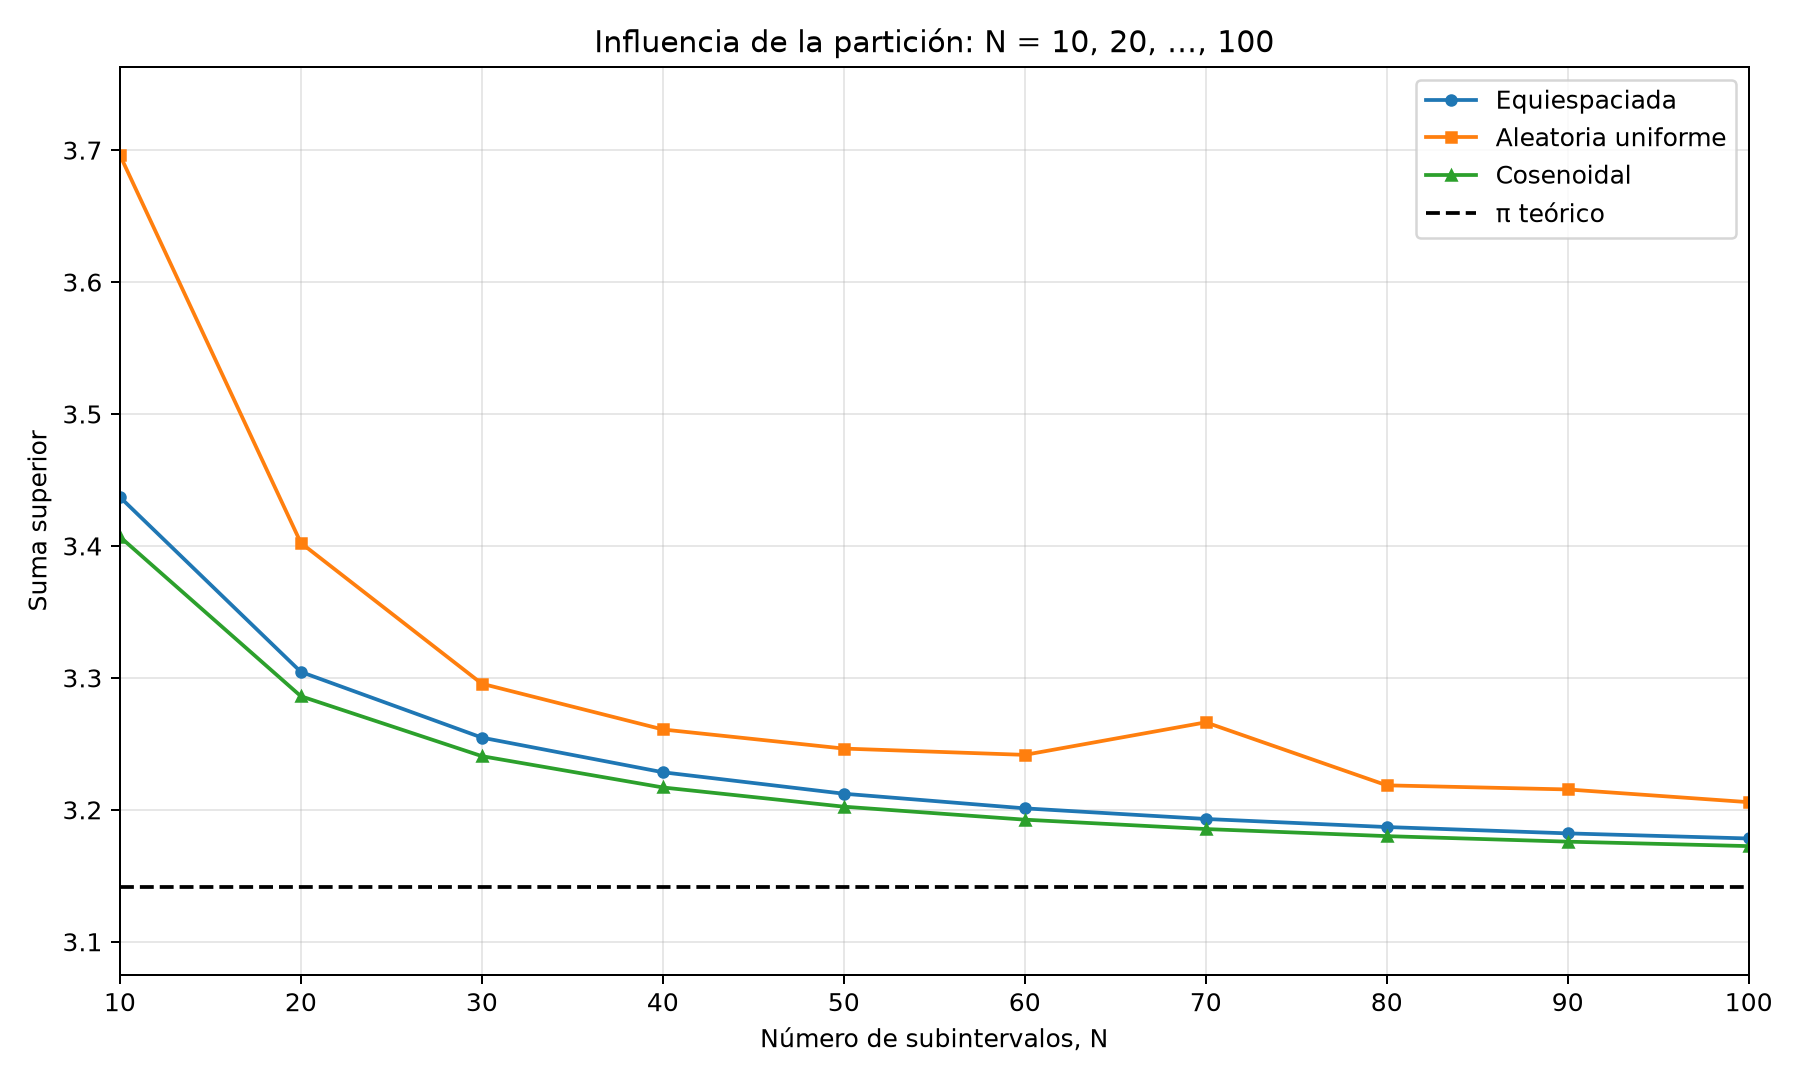
\includegraphics[width=0.88\textwidth]{2grafica_10_a_100.png}
\caption{Suma superior según el tipo de partición para \(N\) entre 10 y 100.}
\label{fig:e2_10a100}
\end{figure}

\begin{figure}[H]
\centering
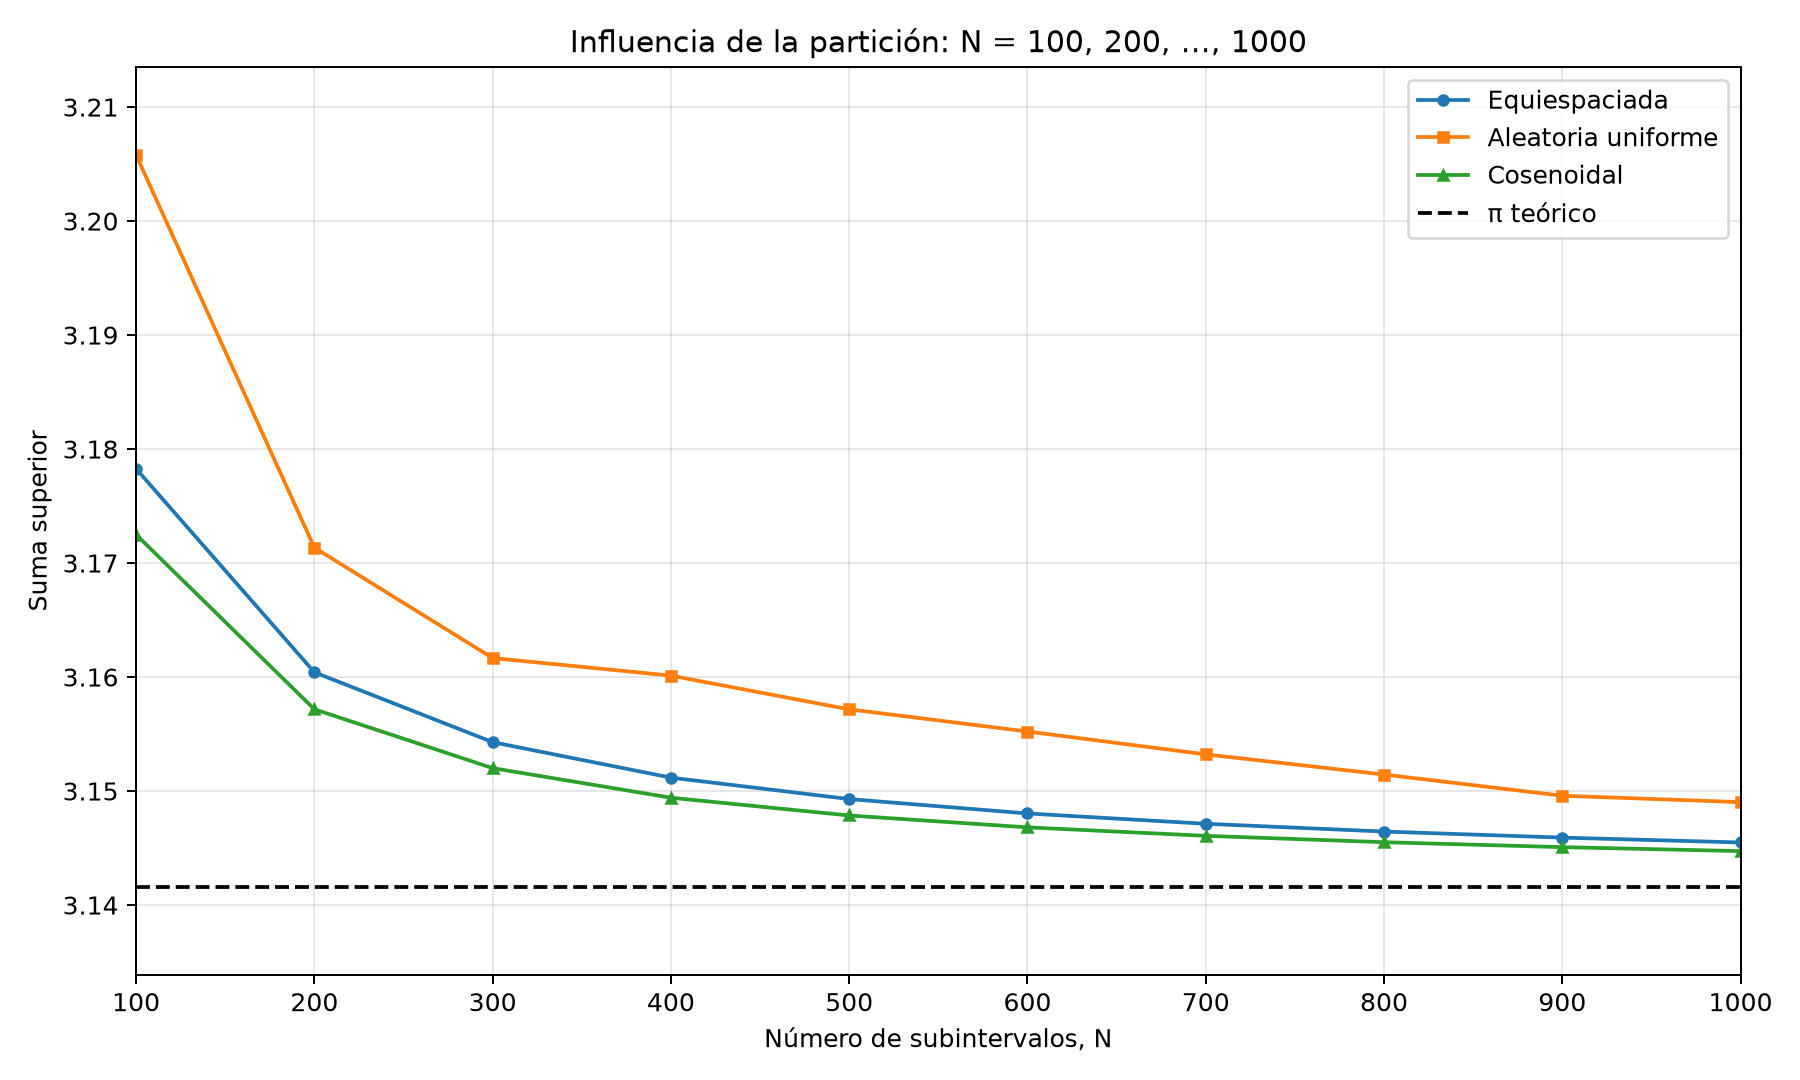
\includegraphics[width=0.88\textwidth]{2grafica_100_a_1000.png}
\caption{Suma superior según el tipo de partición para \(N\) entre 100 y 1000.}
\label{fig:e2_100a1000}
\end{figure}

\begin{figure}[H]
\centering
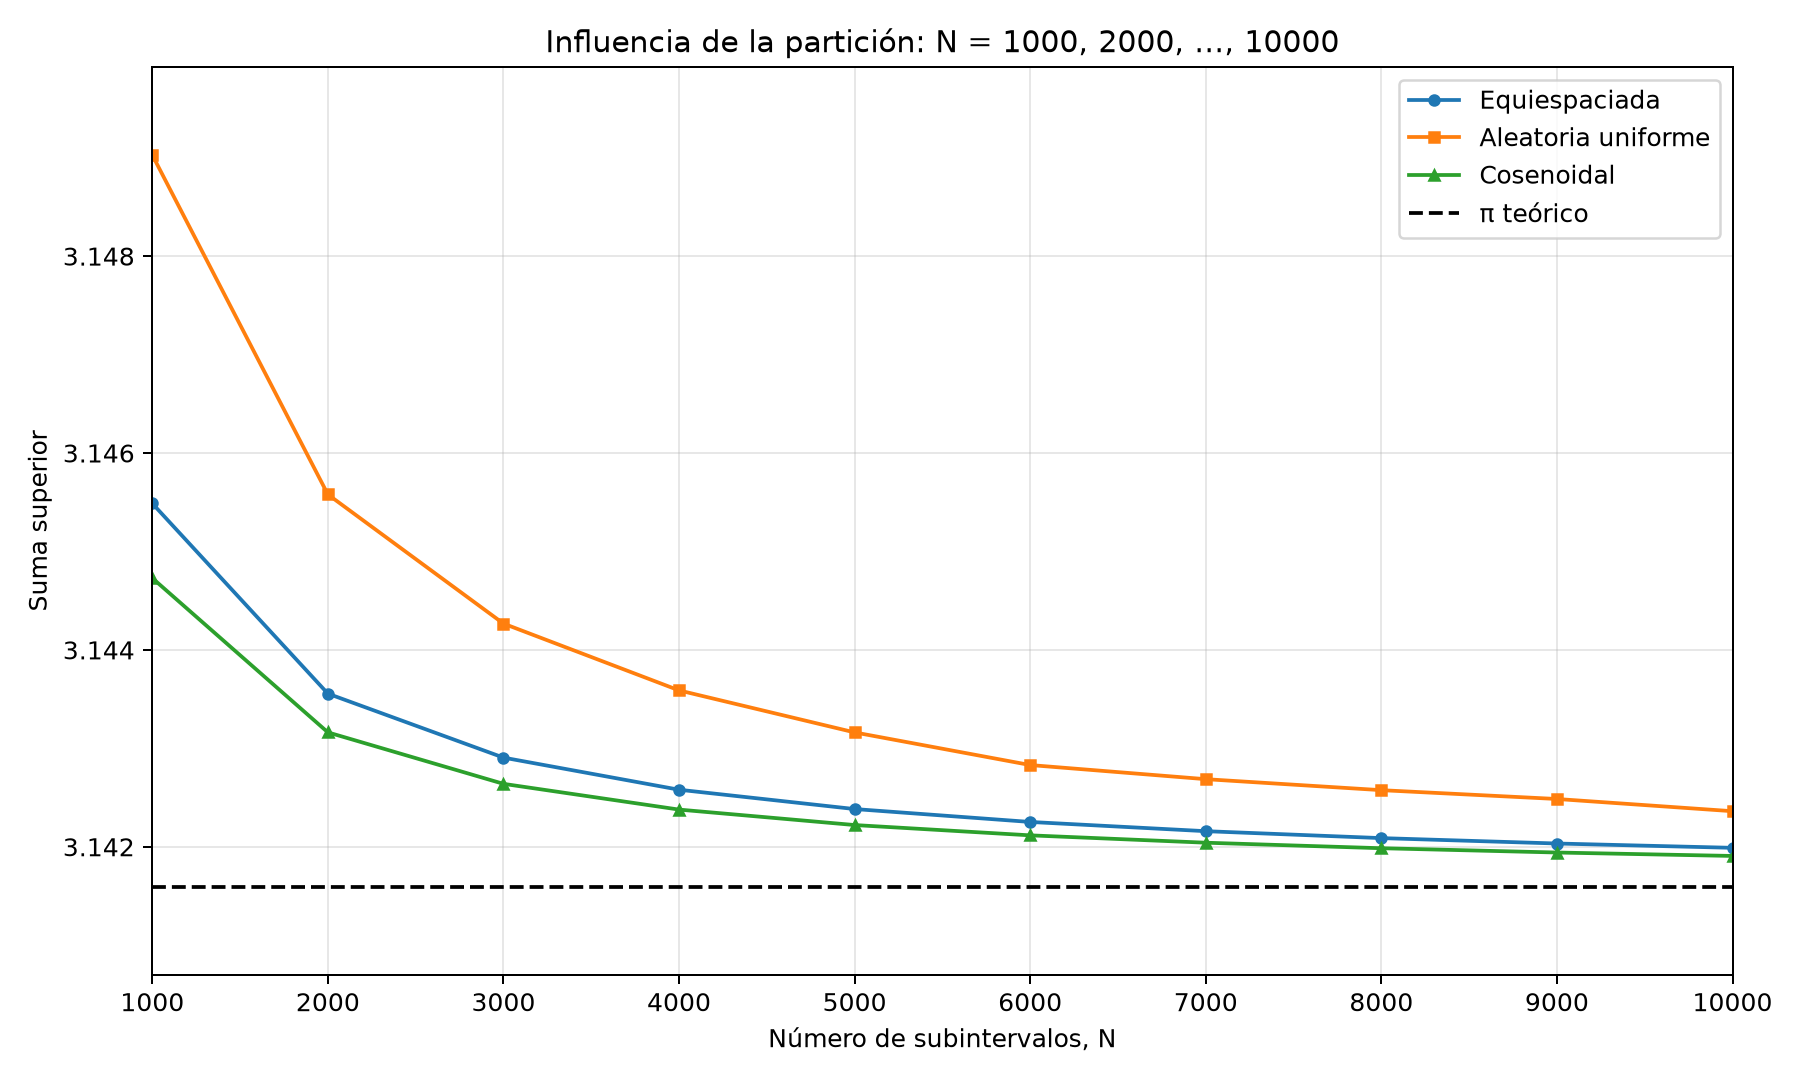
\includegraphics[width=0.88\textwidth]{2grafica_1000_a_10000.png}
\caption{Suma superior según el tipo de partición para \(N\) entre 1000 y 10000.}
\label{fig:e2_1000a10000}
\end{figure}

La consigna también pide graficar la función \(f\) y los rectángulos de la aproximación para cada partición con \(N=100\) (Figura~\ref{fig:e2_rect}). En la equiespaciada todos los rectángulos tienen el mismo ancho; en la aleatoria aparecen rectángulos muy finos junto a otros muy anchos, que sobresalen mucho de la curva; y en la cosenoidal los rectángulos son anchos en el centro y cada vez más finos hacia los bordes.

\begin{figure}[H]
\centering
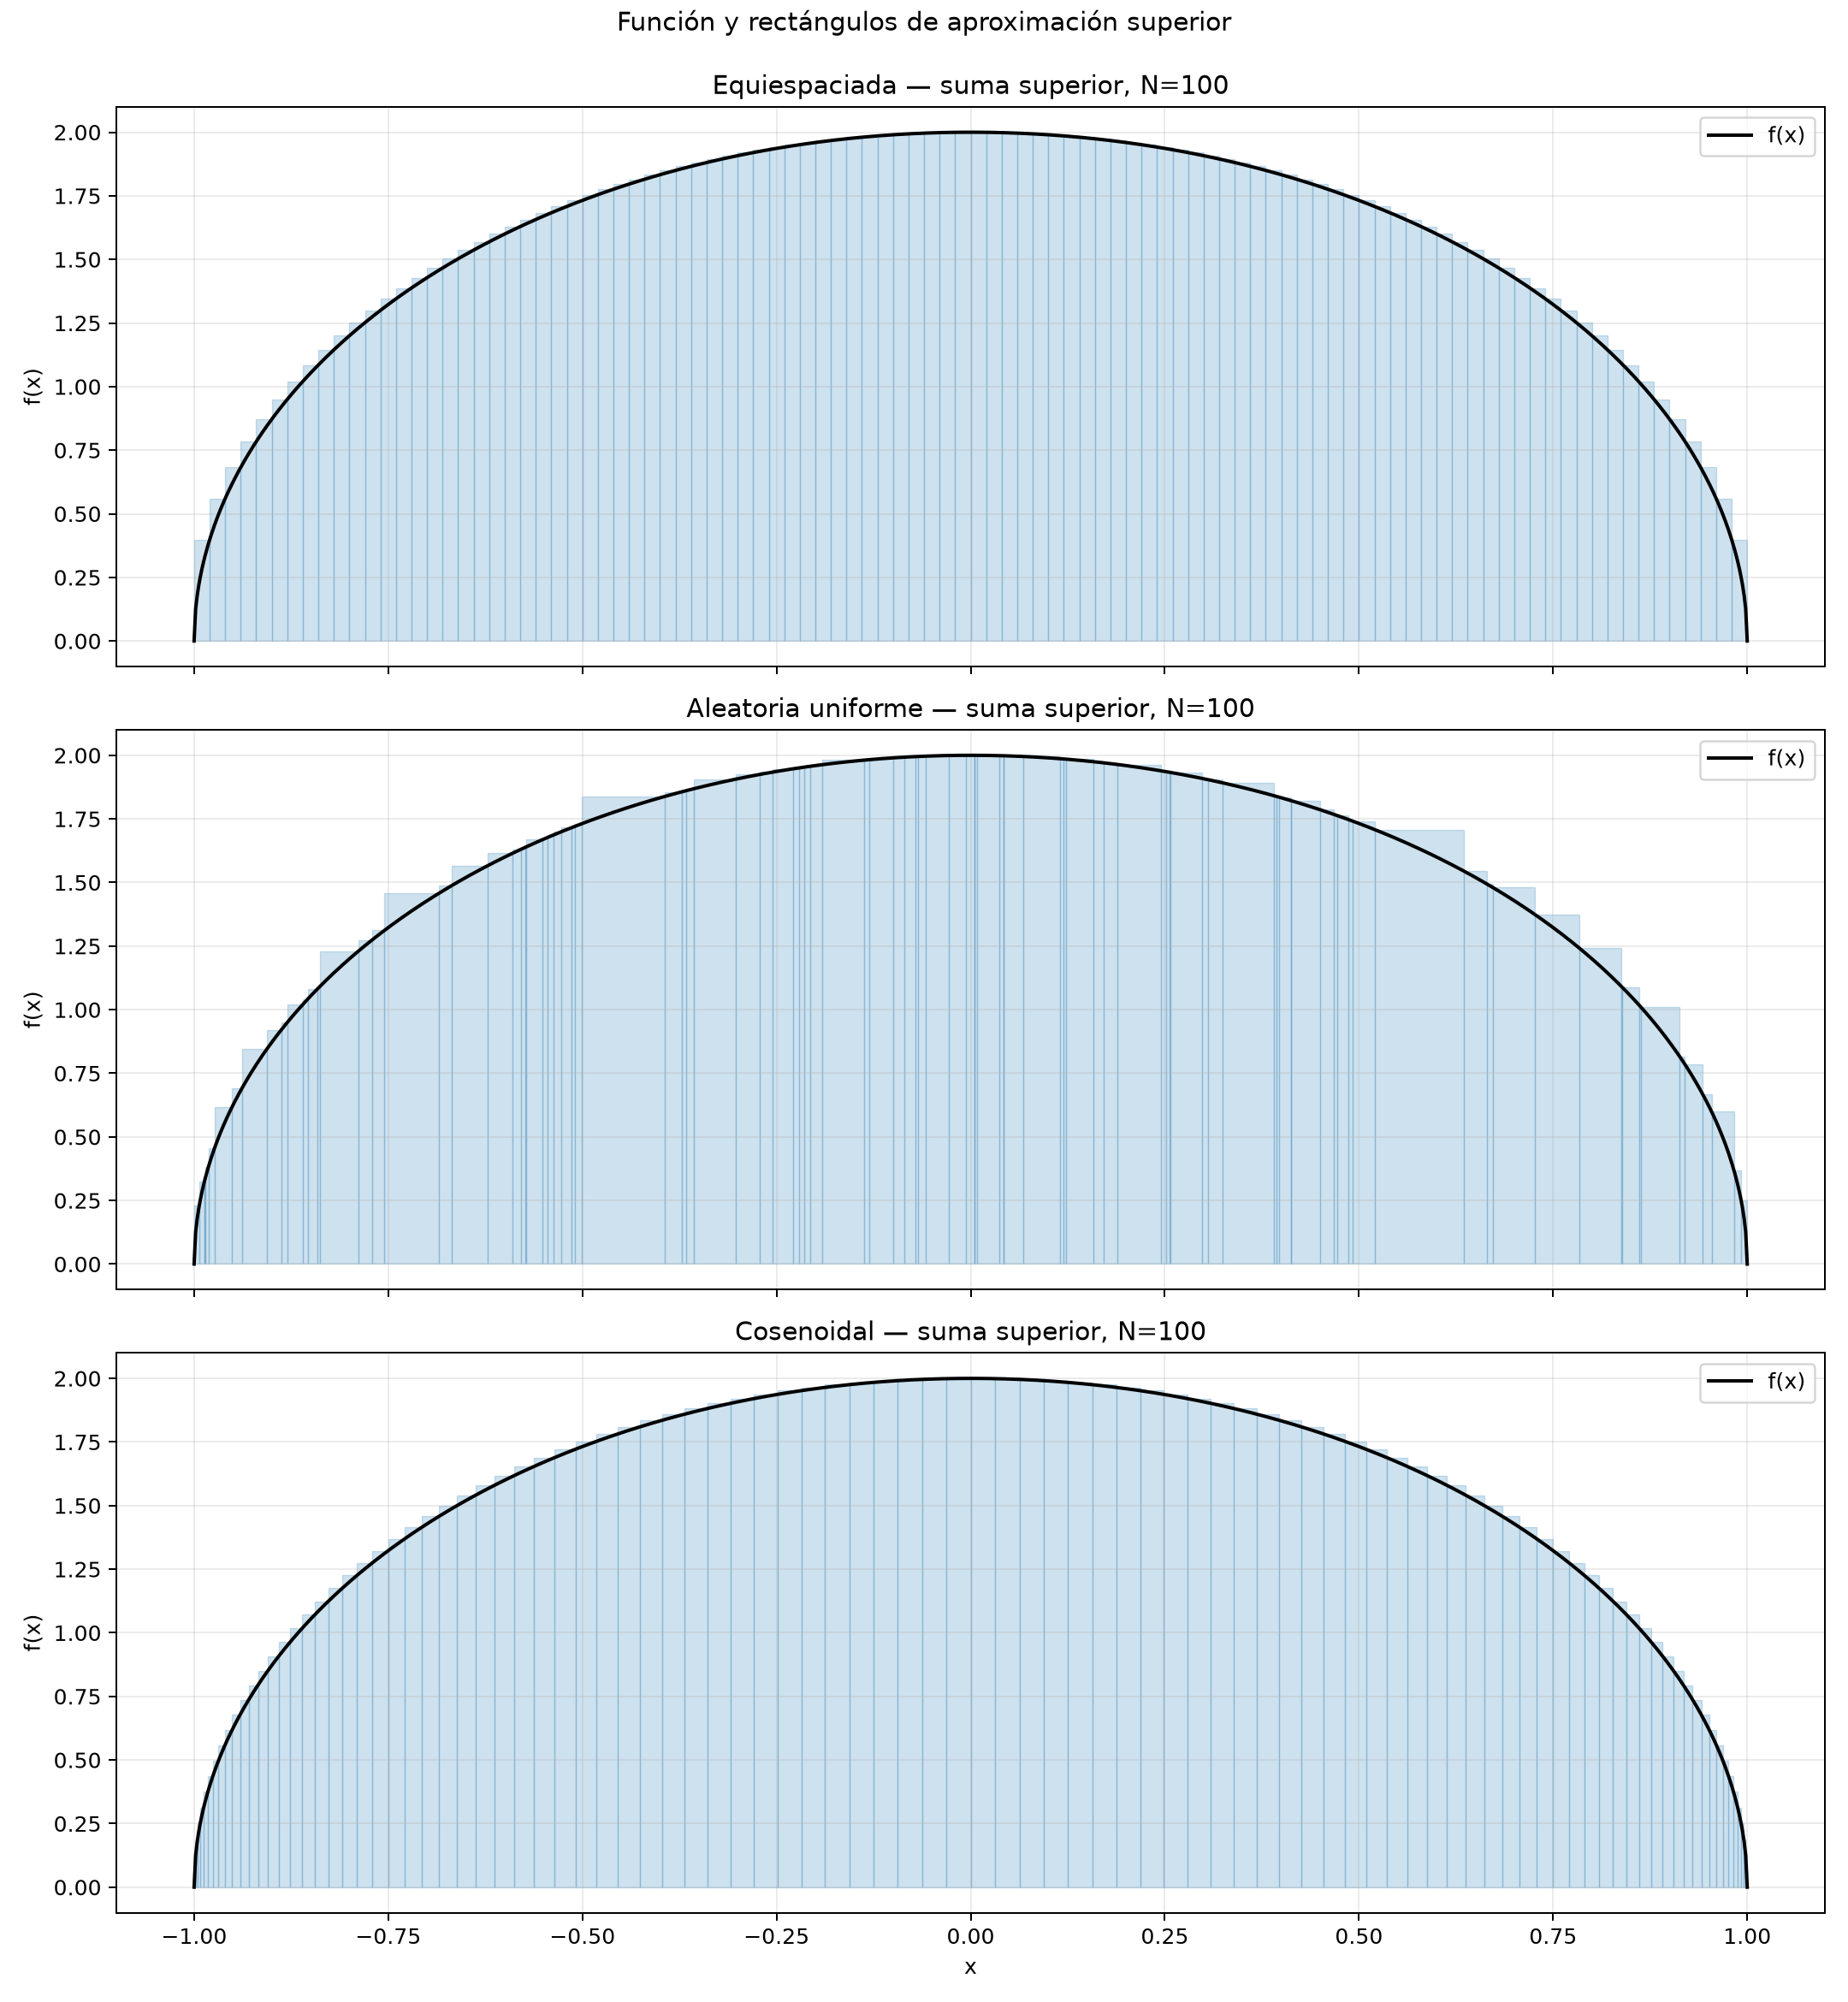
\includegraphics[width=0.85\textwidth]{2rectangulos_N100.png}
\caption{Función \(f\) y rectángulos de la suma superior para cada partición, con \(N=100\).}
\label{fig:e2_rect}
\end{figure}

\subsection{Conclusiones y respuestas analíticas}

\paragraph{¿Qué conclusiones puede tomar? ¿Hay particiones mejores que otras?}
Sí. Las tres particiones convergen a \(\pi\), pero no con la misma precisión: la cosenoidal tiene el menor error en todos los valores de \(N\), seguida por la equiespaciada. La aleatoria uniforme tiene un comportamiento irregular y un error consistentemente mayor (casi el doble que la equiespaciada), porque el azar siempre deja algunos subintervalos desproporcionadamente grandes. Hay que destacar que la mejora de la cosenoidal es moderada: su error es entre un 10\,\% (\(N=10\)) y un 21\,\% (\(N=10000\)) menor que el de la equiespaciada, y en las tres particiones el error disminuye aproximadamente como \(1/N\). Es decir, cambiar la partición reduce el error, pero no cambia la velocidad con la que converge el método.

\paragraph{¿Qué partición dio el mejor resultado? ¿Tiene sentido?}
La partición cosenoidal, \(x_i=\cos\left(\frac{i\pi}{N}\right)\). Tiene sentido: la función \(f(x)=2\sqrt{1-x^2}\) representa una semicircunferencia, cuya pendiente se vuelve vertical en los extremos \(x=\pm1\). En la suma superior, lo que sobra por encima de la curva en cada rectángulo depende de su ancho y de cuánto baja la curva dentro de él. Cerca de los bordes la curva baja muy rápido, así que ahí conviene usar rectángulos finos; en el centro la curva es casi plana y los rectángulos anchos casi no sobresalen. La partición cosenoidal hace exactamente eso: concentra los puntos en los bordes y los separa en el centro.

\paragraph{¿Afecta la geometría de la función a este resultado?}
Sí, la geometría es la explicación. La pendiente vertical en los extremos castiga a las particiones equiespaciada y aleatoria, que dejan subintervalos relativamente grandes justo donde la función cambia más. Los puntos cosenoidales provienen de dividir la circunferencia en ángulos iguales, por lo que se adaptan naturalmente a esta curva. Si la función fuera empinada en el centro y plana en los bordes, juntar los puntos en los extremos no ayudaría: no existe una partición que sea la mejor para todas las funciones, sino que conviene poner más puntos donde la función cambia más rápido.

%=====================================================================
\section{Ejercicio 3: Comparación de métodos}
%=====================================================================

\subsection{Introducción}

En esta sección comparamos tres métodos de integración numérica sobre una misma partición equiespaciada de \([-1,1]\). Como en el Ejercicio 1, \(N\) es la \textbf{cantidad de puntos} de la partición, que forman \(N-1\) subintervalos de ancho
\[
h=\frac{1-(-1)}{N-1}=\frac{2}{N-1},
\qquad x_i=-1+ih,\quad i=0,1,\ldots,N-1.
\]
Los tres métodos son:
\begin{enumerate}
    \item \textbf{Rectángulos (el método usual):} la altura de cada rectángulo es el valor de la función en el extremo izquierdo del subintervalo:
    \[
    R_N=h\sum_{i=0}^{N-2}f(x_i).
    \]
    \item \textbf{Trapecio:} en cada subintervalo se une con una recta los dos puntos de la curva en sus extremos, y se suma el área del trapecio que queda debajo:
    \[
    T_N=\sum_{i=0}^{N-2}\frac{f(x_i)+f(x_{i+1})}{2}\,h.
    \]
    \item \textbf{Punto medio:} la altura de cada rectángulo es el valor de la función en el centro del subintervalo:
    \[
    M_N=h\sum_{i=0}^{N-2}f\!\left(\frac{x_i+x_{i+1}}{2}\right).
    \]
\end{enumerate}
El residuo de cada método se define como \(Q_N-\pi\), donde \(Q_N\) es la aproximación. Un residuo negativo indica que el método subestima la integral y uno positivo, que la sobreestima; para comparar la precisión se mira su valor absoluto.

La Figura~\ref{fig:e3_ilustracion} muestra cómo aproxima el área cada método con solo \(N=6\) puntos.

\begin{figure}[H]
\centering
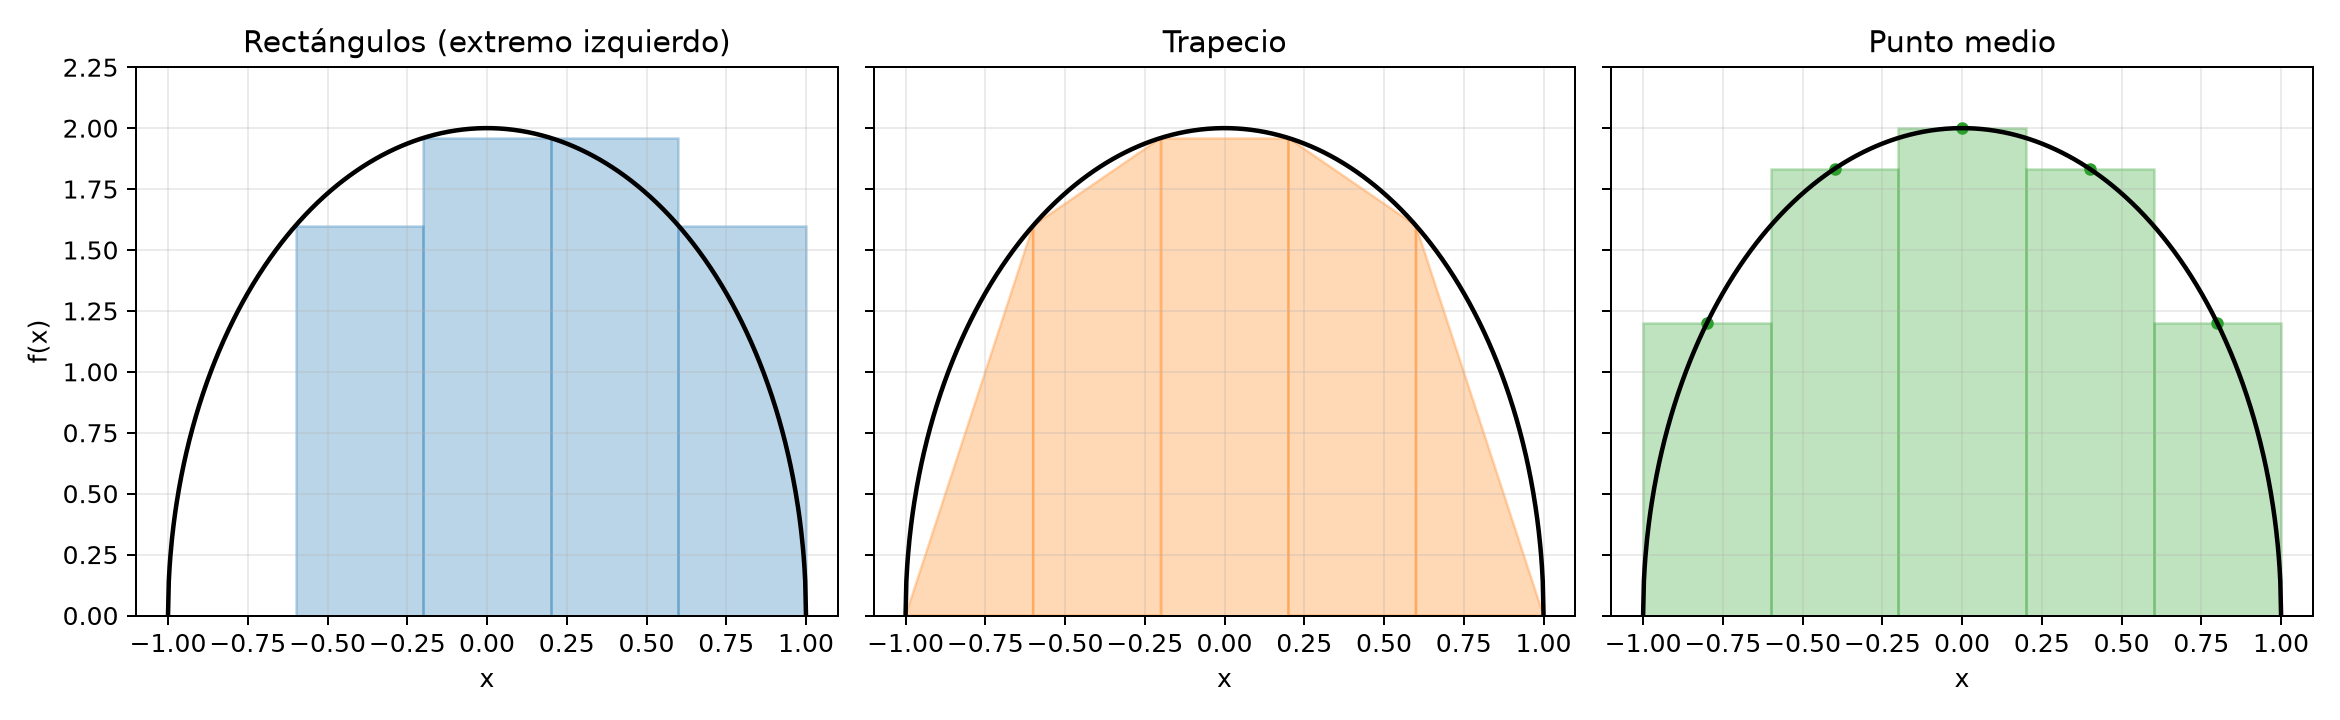
\includegraphics[width=\textwidth]{3metodos_ilustracion.png}
\caption{Aproximación del área con rectángulos (extremo izquierdo), trapecios y punto medio, con \(N=6\) puntos.}
\label{fig:e3_ilustracion}
\end{figure}

\subsection{Implementación en Python}

A continuación se muestra el código implementado en Python para construir la partición y calcular las tres aproximaciones (versión resumida; las funciones que imprimen las tablas, guardan los CSV y dibujan las gráficas se omiten):

\begin{lstlisting}[language=Python, caption={Código fuente del Ejercicio 3 (versión resumida)}]
import math

A = -1.0
B = 1.0
PI = math.pi

RANGOS_N = {
    "10_a_100": range(10, 101, 10),
    "100_a_1000": range(100, 1001, 100),
    "1000_a_10000": range(1000, 10001, 1000),
}

def f(x: float) -> float:
    return 2.0 * math.sqrt(max(0.0, 1.0 - x * x))

def particion_equiespaciada(n: int) -> list[float]:
    """N puntos equiespaciados, incluyendo -1 y 1 (N-1 subintervalos)."""
    if not isinstance(n, int) or isinstance(n, bool) or n < 2:
        raise ValueError("N debe ser un entero de al menos 2 puntos")
    return [A + (B - A) * i / (n - 1) for i in range(n)]

def metodo_rectangulos(puntos: list[float]) -> float:
    suma = 0.0
    for x_izq, x_der in zip(puntos, puntos[1:]):
        suma += f(x_izq) * (x_der - x_izq)
    return suma

def metodo_trapecio(puntos: list[float]) -> float:
    suma = 0.0
    for x_izq, x_der in zip(puntos, puntos[1:]):
        suma += (f(x_izq) + f(x_der)) * (x_der - x_izq) / 2.0
    return suma

def metodo_punto_medio(puntos: list[float]) -> float:
    suma = 0.0
    for x_izq, x_der in zip(puntos, puntos[1:]):
        punto_medio = (x_izq + x_der) / 2.0
        suma += f(punto_medio) * (x_der - x_izq)
    return suma

def generar_registros(valores_n: list[int]) -> list[dict[str, float | int]]:
    metodos = {
        "rectangulos": metodo_rectangulos,
        "trapecio": metodo_trapecio,
        "punto_medio": metodo_punto_medio,
    }
    registros = []
    for n in valores_n:
        puntos = particion_equiespaciada(n)
        registro: dict[str, float | int] = {"N": n}
        for nombre, funcion_metodo in metodos.items():
            aprox = funcion_metodo(puntos)
            registro[f"aprox_{nombre}"] = aprox
            registro[f"residuo_{nombre}"] = aprox - PI
        registros.append(registro)
    return registros
\end{lstlisting}

\subsection{Tablas comparativas de resultados}

Las siguientes tablas muestran la aproximación de cada método y su residuo. Como los residuos se hacen muy chicos, se escriben en notación científica.

\begin{table}[H]
\centering
\caption{Aproximación según el método, \(N\) entre 10 y 100, en incrementos de 10.}
\label{tab:e3_10a100}
\footnotesize
\setlength{\tabcolsep}{3pt}
\begin{tabular}{r r r r r r r}
\toprule
\(N\) & Rectángulos & Residuo & Trapecio & Residuo & Punto medio & Residuo \\
\midrule
10    & 3.01923183 & \(-1.2236\times10^{-1}\) & 3.01923183 & \(-1.2236\times10^{-1}\) & 3.17713893 & \(+3.5546\times10^{-2}\) \\
20    & 3.10155965 & \(-4.0033\times10^{-2}\) & 3.10155965 & \(-4.0033\times10^{-2}\) & 3.15327255 & \(+1.1680\times10^{-2}\) \\
30    & 3.12033906 & \(-2.1254\times10^{-2}\) & 3.12033906 & \(-2.1254\times10^{-2}\) & 3.14780184 & \(+6.2092\times10^{-3}\) \\
40    & 3.12795728 & \(-1.3635\times10^{-2}\) & 3.12795728 & \(-1.3635\times10^{-2}\) & 3.14557880 & \(+3.9861\times10^{-3}\) \\
50    & 3.13190745 & \(-9.6852\times10^{-3}\) & 3.13190745 & \(-9.6852\times10^{-3}\) & 3.14442511 & \(+2.8325\times10^{-3}\) \\
60    & 3.13426075 & \(-7.3319\times10^{-3}\) & 3.13426075 & \(-7.3319\times10^{-3}\) & 3.14373743 & \(+2.1448\times10^{-3}\) \\
70    & 3.13579454 & \(-5.7981\times10^{-3}\) & 3.13579454 & \(-5.7981\times10^{-3}\) & 3.14328906 & \(+1.6964\times10^{-3}\) \\
80    & 3.13685931 & \(-4.7333\times10^{-3}\) & 3.13685931 & \(-4.7333\times10^{-3}\) & 3.14297772 & \(+1.3851\times10^{-3}\) \\
90    & 3.13763387 & \(-3.9588\times10^{-3}\) & 3.13763387 & \(-3.9588\times10^{-3}\) & 3.14275119 & \(+1.1585\times10^{-3}\) \\
100   & 3.13821804 & \(-3.3746\times10^{-3}\) & 3.13821804 & \(-3.3746\times10^{-3}\) & 3.14258032 & \(+9.8766\times10^{-4}\) \\
\bottomrule
\end{tabular}
\end{table}

\begin{table}[H]
\centering
\caption{Aproximación según el método, \(N\) entre 100 y 1000, en incrementos de 100.}
\label{tab:e3_100a1000}
\footnotesize
\setlength{\tabcolsep}{3pt}
\begin{tabular}{r r r r r r r}
\toprule
\(N\) & Rectángulos & Residuo & Trapecio & Residuo & Punto medio & Residuo \\
\midrule
100   & 3.13821804 & \(-3.3746\times10^{-3}\) & 3.13821804 & \(-3.3746\times10^{-3}\) & 3.14258032 & \(+9.8766\times10^{-4}\) \\
200   & 3.14040816 & \(-1.1845\times10^{-3}\) & 3.14040816 & \(-1.1845\times10^{-3}\) & 3.14193945 & \(+3.4680\times10^{-4}\) \\
300   & 3.14094945 & \(-6.4321\times10^{-4}\) & 3.14094945 & \(-6.4321\times10^{-4}\) & 3.14178100 & \(+1.8834\times10^{-4}\) \\
400   & 3.14117538 & \(-4.1727\times10^{-4}\) & 3.14117538 & \(-4.1727\times10^{-4}\) & 3.14171485 & \(+1.2219\times10^{-4}\) \\
500   & 3.14129429 & \(-2.9836\times10^{-4}\) & 3.14129429 & \(-2.9836\times10^{-4}\) & 3.14168003 & \(+8.7375\times10^{-5}\) \\
600   & 3.14136579 & \(-2.2686\times10^{-4}\) & 3.14136579 & \(-2.2686\times10^{-4}\) & 3.14165909 & \(+6.6438\times10^{-5}\) \\
700   & 3.14141269 & \(-1.7997\times10^{-4}\) & 3.14141269 & \(-1.7997\times10^{-4}\) & 3.14164536 & \(+5.2705\times10^{-5}\) \\
800   & 3.14144539 & \(-1.4726\times10^{-4}\) & 3.14144539 & \(-1.4726\times10^{-4}\) & 3.14163578 & \(+4.3128\times10^{-5}\) \\
900   & 3.14146926 & \(-1.2339\times10^{-4}\) & 3.14146926 & \(-1.2339\times10^{-4}\) & 3.14162879 & \(+3.6137\times10^{-5}\) \\
1000  & 3.14148732 & \(-1.0533\times10^{-4}\) & 3.14148732 & \(-1.0533\times10^{-4}\) & 3.14162350 & \(+3.0849\times10^{-5}\) \\
\bottomrule
\end{tabular}
\end{table}

\begin{table}[H]
\centering
\caption{Aproximación según el método, \(N\) entre 1000 y 10000, en incrementos de 1000.}
\label{tab:e3_1000a10000}
\footnotesize
\setlength{\tabcolsep}{3pt}
\begin{tabular}{r r r r r r r}
\toprule
\(N\) & Rectángulos & Residuo & Trapecio & Residuo & Punto medio & Residuo \\
\midrule
1000  & 3.14148732 & \(-1.0533\times10^{-4}\) & 3.14148732 & \(-1.0533\times10^{-4}\) & 3.14162350 & \(+3.0849\times10^{-5}\) \\
2000  & 3.14155544 & \(-3.7215\times10^{-5}\) & 3.14155544 & \(-3.7215\times10^{-5}\) & 3.14160355 & \(+1.0899\times10^{-5}\) \\
3000  & 3.14157240 & \(-2.0252\times10^{-5}\) & 3.14157240 & \(-2.0252\times10^{-5}\) & 3.14159859 & \(+5.9316\times10^{-6}\) \\
4000  & 3.14157950 & \(-1.3153\times10^{-5}\) & 3.14157950 & \(-1.3153\times10^{-5}\) & 3.14159651 & \(+3.8522\times10^{-6}\) \\
5000  & 3.14158324 & \(-9.4106\times10^{-6}\) & 3.14158324 & \(-9.4106\times10^{-6}\) & 3.14159541 & \(+2.7562\times10^{-6}\) \\
6000  & 3.14158550 & \(-7.1585\times10^{-6}\) & 3.14158550 & \(-7.1585\times10^{-6}\) & 3.14159475 & \(+2.0967\times10^{-6}\) \\
7000  & 3.14158697 & \(-5.6805\times10^{-6}\) & 3.14158697 & \(-5.6805\times10^{-6}\) & 3.14159432 & \(+1.6638\times10^{-6}\) \\
8000  & 3.14158800 & \(-4.6493\times10^{-6}\) & 3.14158800 & \(-4.6493\times10^{-6}\) & 3.14159402 & \(+1.3617\times10^{-6}\) \\
9000  & 3.14158876 & \(-3.8963\times10^{-6}\) & 3.14158876 & \(-3.8963\times10^{-6}\) & 3.14159379 & \(+1.1412\times10^{-6}\) \\
10000 & 3.14158933 & \(-3.3267\times10^{-6}\) & 3.14158933 & \(-3.3267\times10^{-6}\) & 3.14159363 & \(+9.7435\times10^{-7}\) \\
\bottomrule
\end{tabular}
\end{table}

Lo primero que llama la atención es que \textbf{rectángulos y trapecio dan exactamente el mismo resultado} en todas las filas. No es un error del programa: como \(f(-1)=f(1)=0\), el primer rectángulo tiene altura cero, y en la fórmula del trapecio los dos extremos también aportan cero, así que las dos fórmulas terminan sumando exactamente los mismos términos:
\[
R_N=h\sum_{i=1}^{N-2}f(x_i)=T_N.
\]
Además, rectángulos y trapecio siempre quedan por debajo de \(\pi\) (residuo negativo), mientras que el punto medio siempre queda por encima (residuo positivo) y con un error absoluto unas tres veces menor.

\subsection{Análisis de las gráficas}

Las gráficas muestran las tres aproximaciones junto con el valor exacto \(\pi\) para cada rango de \(N\). Las curvas de rectángulos y trapecio aparecen superpuestas porque sus valores coinciden.

\begin{figure}[H]
\centering
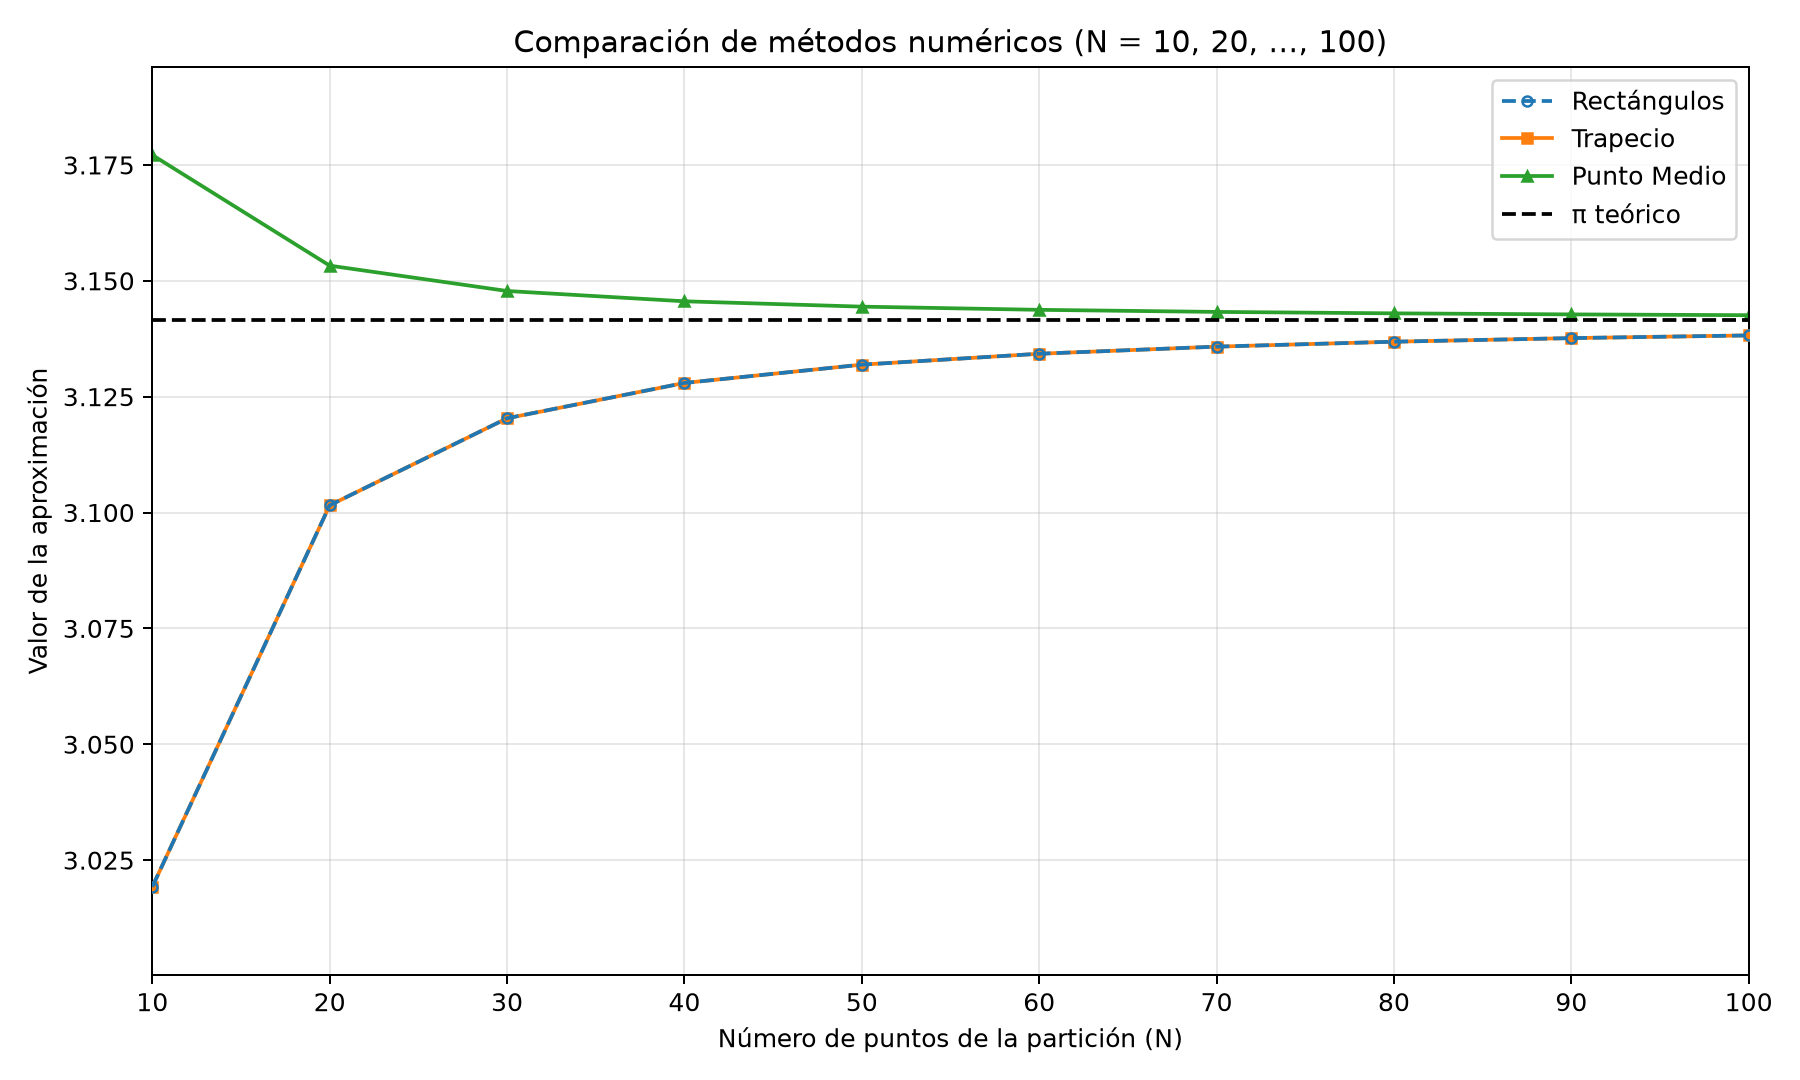
\includegraphics[width=0.88\textwidth]{3grafica_metodos_10_a_100.png}
\caption{Aproximación según el método para \(N\) entre 10 y 100.}
\label{fig:e3_10a100}
\end{figure}

\begin{figure}[H]
\centering
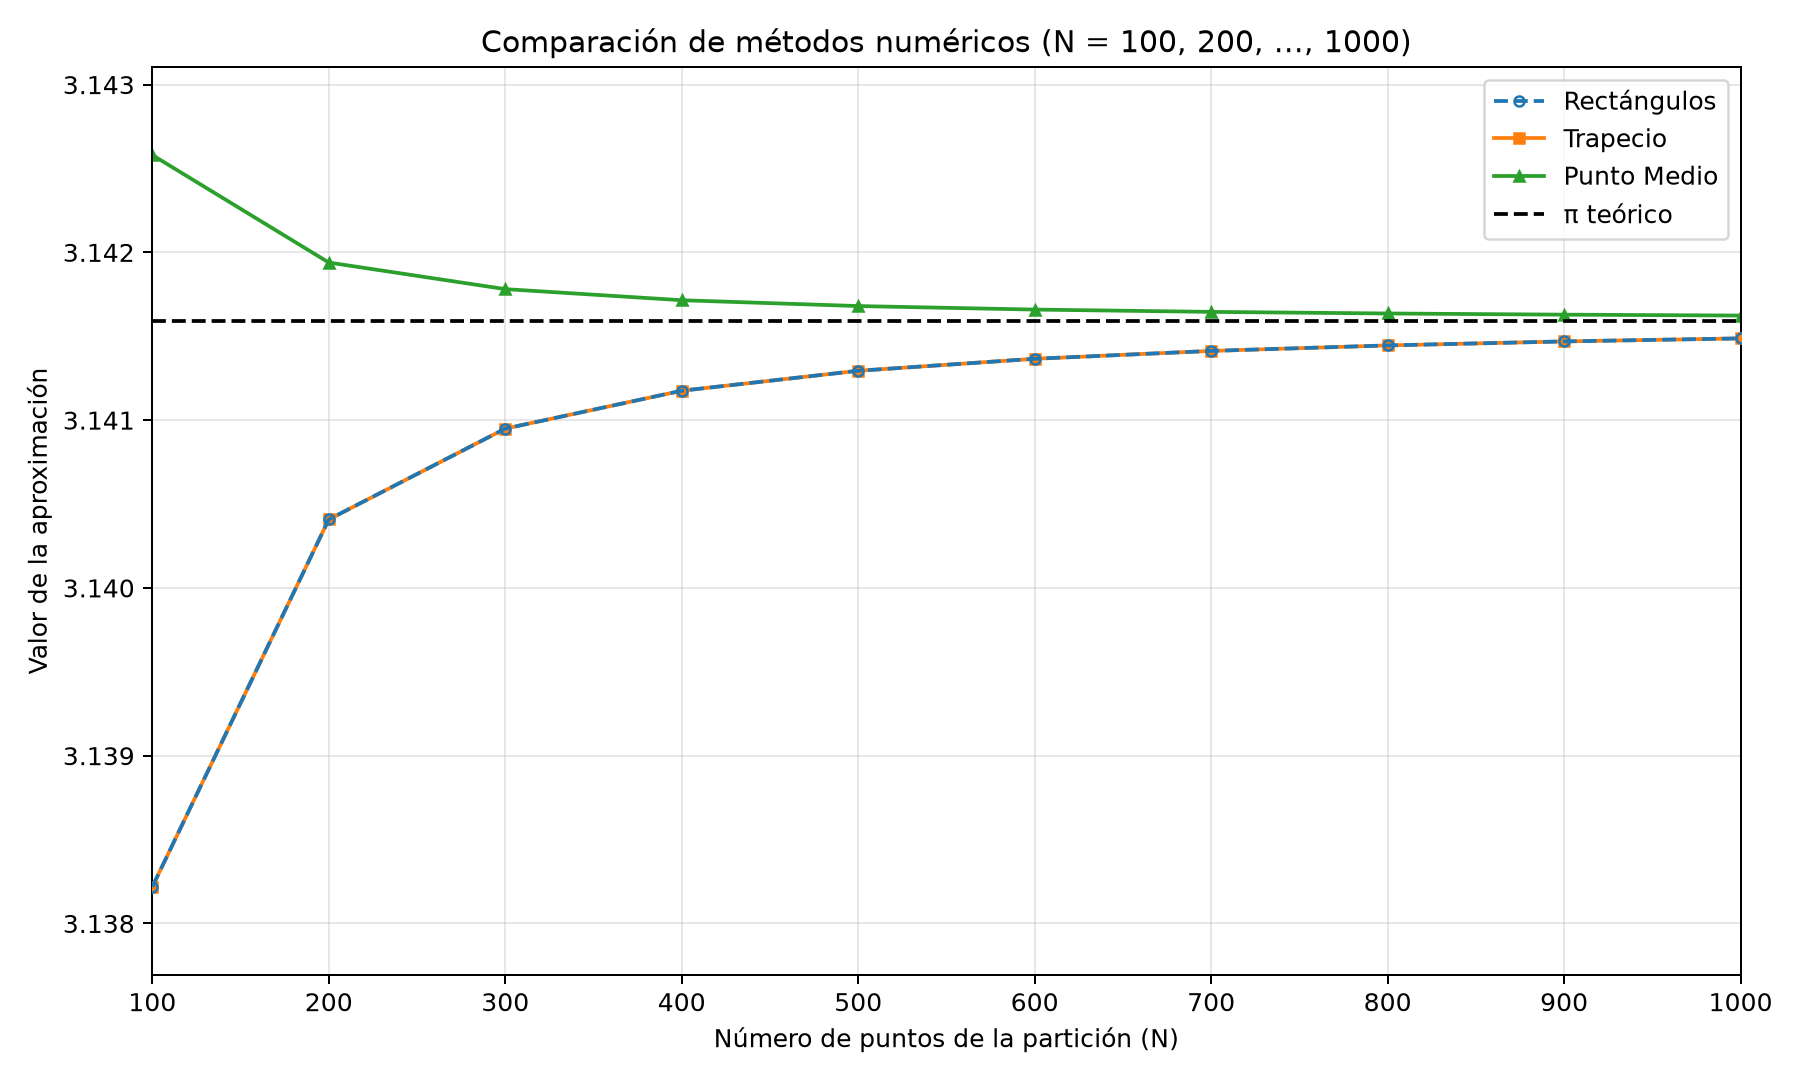
\includegraphics[width=0.88\textwidth]{3grafica_metodos_100_a_1000.png}
\caption{Aproximación según el método para \(N\) entre 100 y 1000.}
\label{fig:e3_100a1000}
\end{figure}

\begin{figure}[H]
\centering
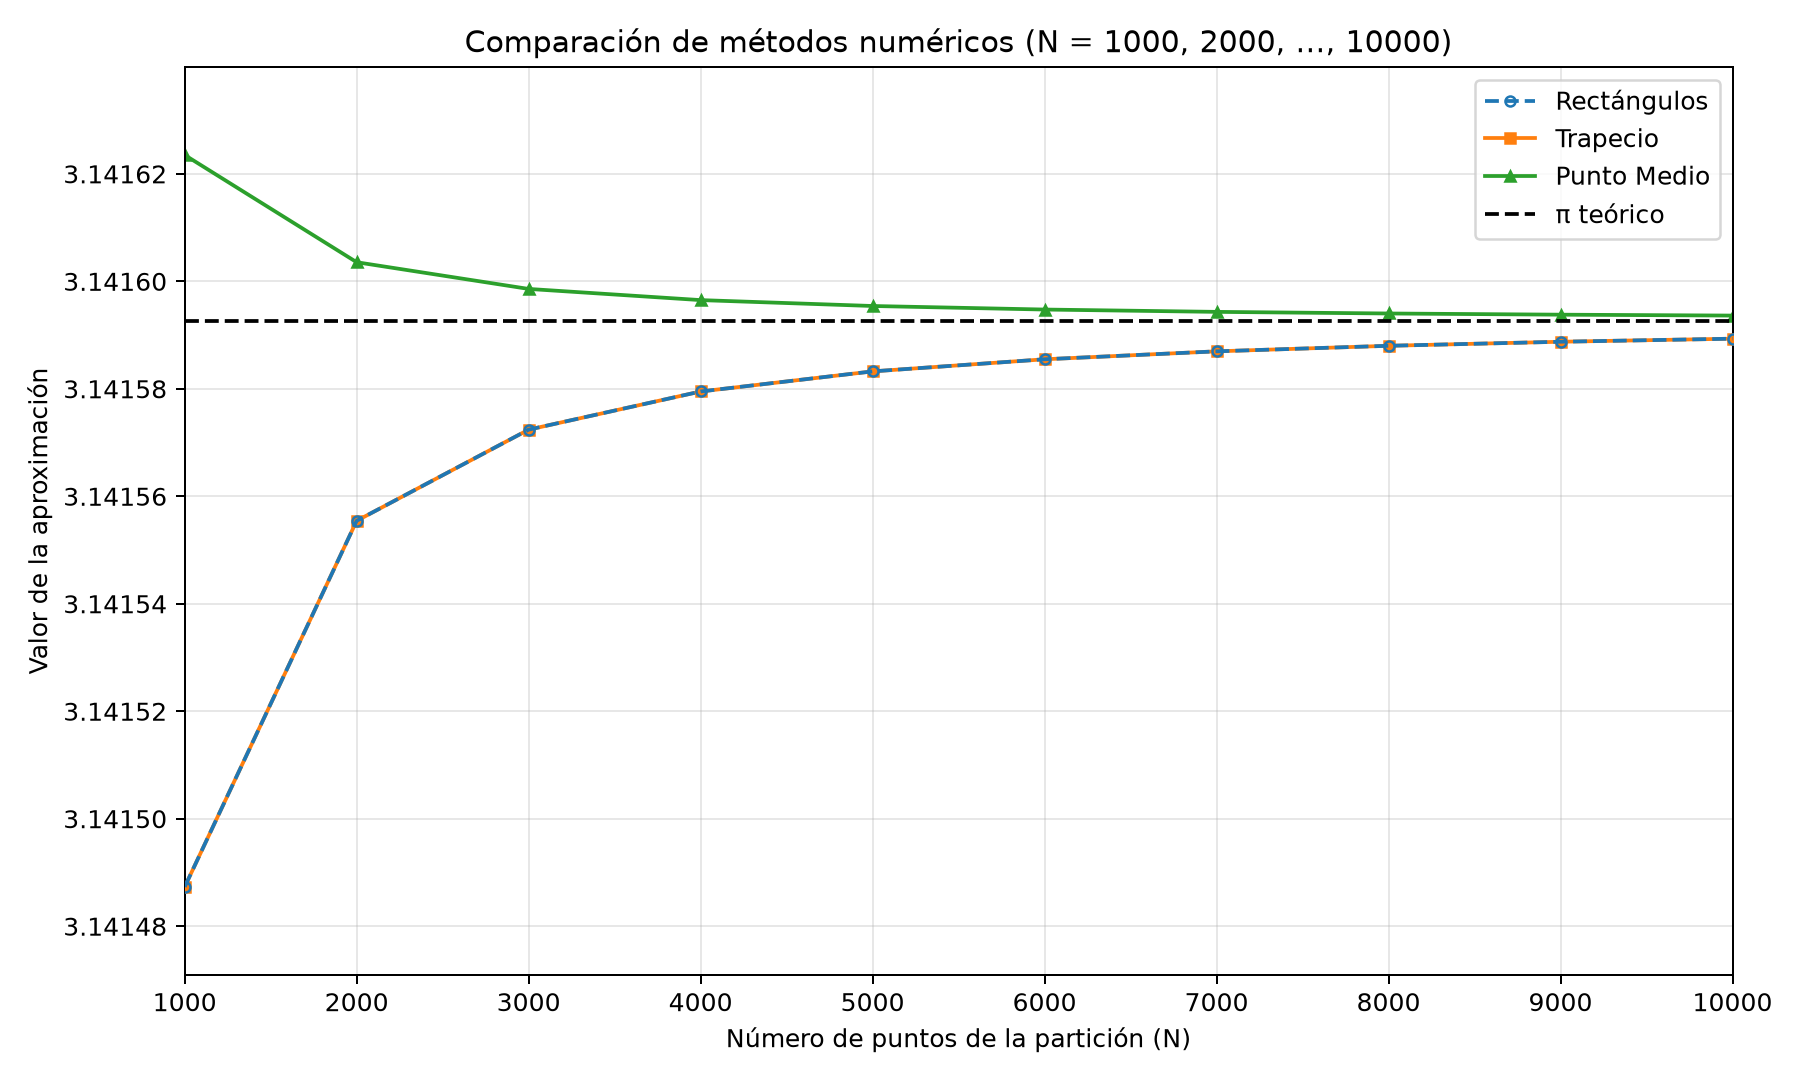
\includegraphics[width=0.88\textwidth]{3grafica_metodos_1000_a_10000.png}
\caption{Aproximación según el método para \(N\) entre 1000 y 10000.}
\label{fig:e3_1000a10000}
\end{figure}

Para ver mejor qué tan rápido baja el error, la Figura~\ref{fig:e3_log} muestra el valor absoluto del residuo en escala logarítmica (cada marca de los ejes representa multiplicar por 10).

\begin{figure}[H]
\centering
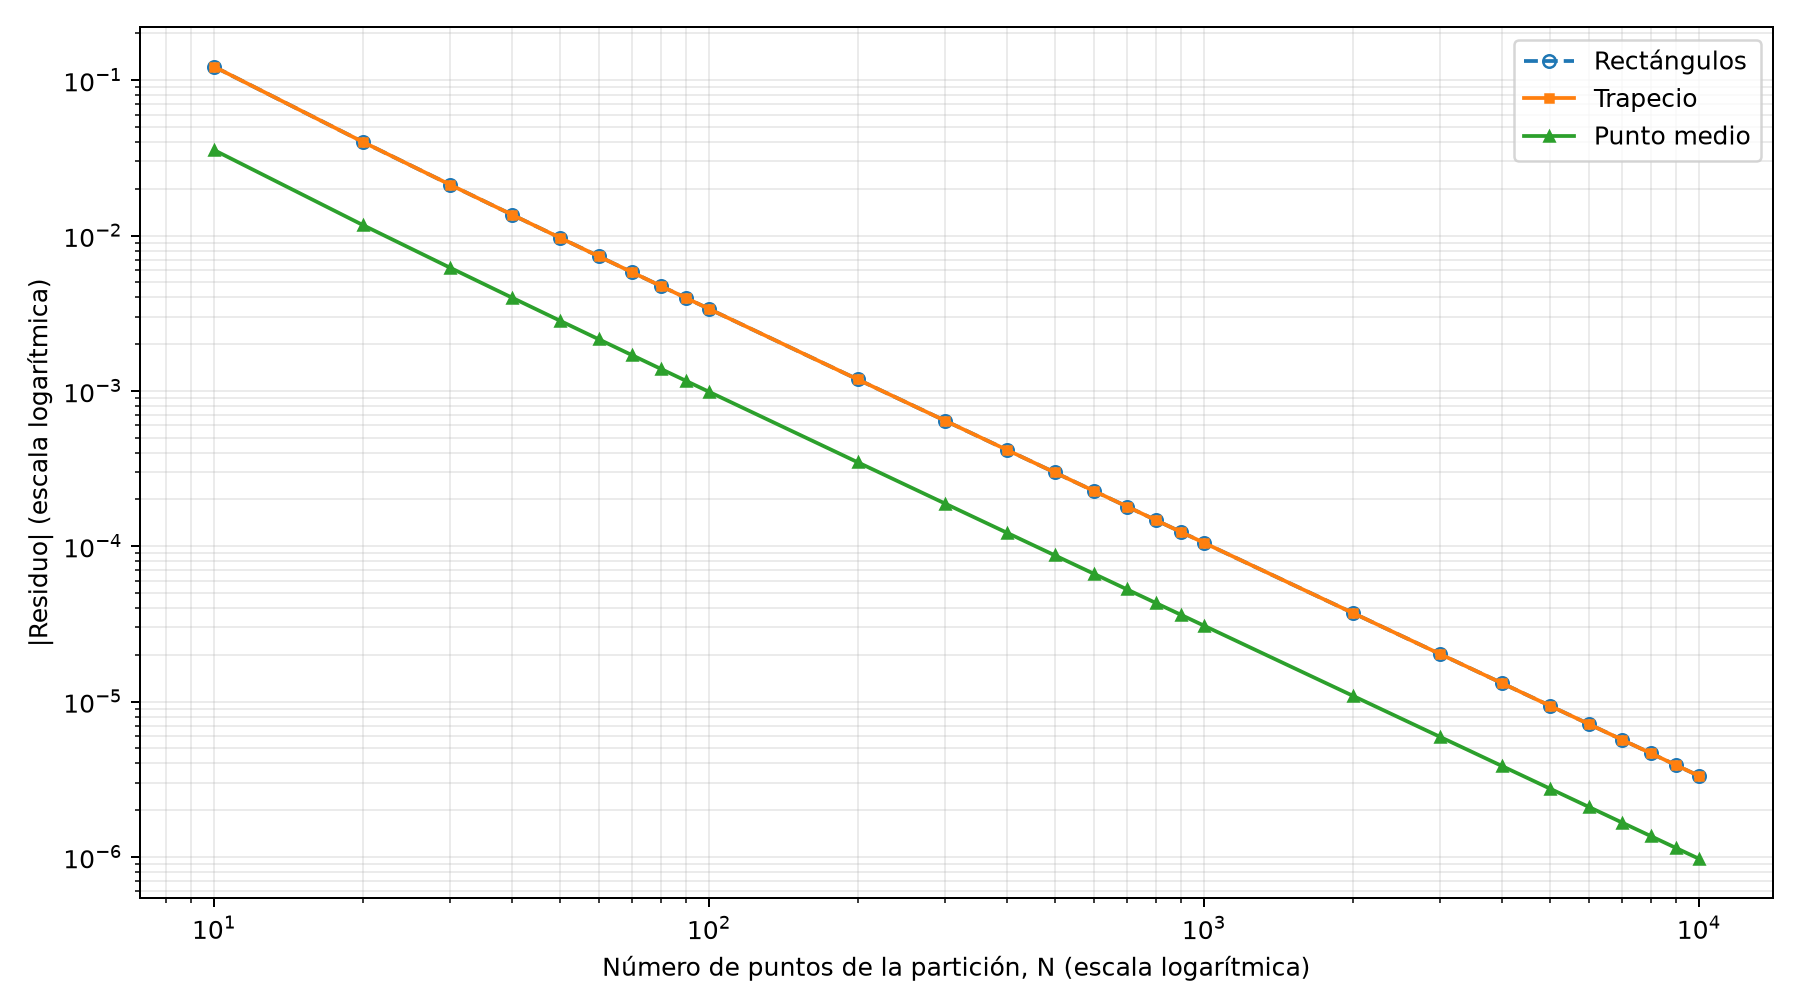
\includegraphics[width=0.88\textwidth]{3errores_log.png}
\caption{Valor absoluto del residuo de cada método según \(N\), en escala logarítmica.}
\label{fig:e3_log}
\end{figure}

Las tres líneas son rectas y paralelas: cada vez que \(N\) se multiplica por 10, el error se divide aproximadamente por 32 (por ejemplo, el residuo del trapecio pasa de \(3.37\times10^{-3}\) con \(N=100\) a \(1.05\times10^{-4}\) con \(N=1000\)). Esto es mucho mejor que las sumas de Darboux de los Ejercicios 1 y 2, donde el error solo se dividía por 10. Con \(N=10000\), el trapecio tiene un error de \(3.3\times10^{-6}\), unas 100 veces menor que el de la suma superior con la misma partición (\(4.0\times10^{-4}\)).

\subsection{Conclusiones y respuestas analíticas}

\paragraph{¿Qué método dio mejores resultados?}
El \textbf{punto medio}. En todos los valores de \(N\) su residuo es el más chico en valor absoluto: aproximadamente un 29\,\% del error del trapecio (por ejemplo, \(9.88\times10^{-4}\) contra \(3.37\times10^{-3}\) con \(N=100\)). Rectángulos y trapecio quedan empatados, porque en este problema dan exactamente el mismo resultado.

\paragraph{¿Hay métodos mejores que otros?}
Sí, pero hay que matizarlo. En general, el trapecio es mejor que los rectángulos, porque reemplaza la ``escalera'' de rectángulos por segmentos que siguen la inclinación de la curva. En este ejercicio esa ventaja no se ve, porque la función vale cero en los dos extremos del intervalo y las dos fórmulas coinciden. Si la función no se anulara en los extremos, los resultados serían distintos. El punto medio, en cambio, sí resulta mejor que los otros dos para esta función.

\paragraph{Justificación geométrica.}
La clave es que la función es \textbf{cóncava hacia abajo} (tiene forma de cúpula):
\[
f''(x)=-\frac{2}{(1-x^2)^{3/2}}<0,\qquad -1<x<1.
\]
\begin{itemize}
    \item \textbf{Trapecio:} el lado de arriba de cada trapecio es una cuerda que une dos puntos de la curva. En una curva cóncava hacia abajo, las cuerdas quedan siempre \textbf{por debajo} de la curva, así que cada trapecio deja un pequeño hueco sin cubrir y la suma total queda por debajo de \(\pi\) (Figura~\ref{fig:e3_ilustracion}, centro).
    \item \textbf{Punto medio:} el área del rectángulo de punto medio es igual al área del trapecio que se forma con la \textbf{recta tangente} a la curva en el centro del subintervalo (lo que el rectángulo agrega de un lado de la tangente lo quita del otro). En una curva cóncava hacia abajo, la tangente queda \textbf{por encima} de la curva, así que el punto medio sobreestima la integral y su residuo es positivo.
    \item \textbf{¿Por qué el punto medio se equivoca menos?} Cerca del centro del subintervalo, la tangente se ``pega'' a la curva mucho más que la cuerda, que solo la toca en los extremos. Por eso el espacio entre la tangente y la curva es más chico que el espacio entre la cuerda y la curva. En funciones suaves el error del punto medio suele ser la mitad del error del trapecio; en nuestra función resultó todavía menor (alrededor del 29\,\%).
\end{itemize}

Por último, el error de los tres métodos baja a un ritmo de aproximadamente \(N^{-1.5}\) (dividido por 32 cada vez que \(N\) se multiplica por 10), y no como \(N^{-2}\), que es lo habitual para el trapecio y el punto medio. Esto también se explica por la geometría: en los extremos \(x=\pm1\) la curva cae en vertical, y ahí ninguna recta (ni la cuerda ni la tangente) la puede seguir bien, así que la mayor parte del error se concentra en los subintervalos de los bordes.

%=====================================================================
\section{Conclusiones generales}
%=====================================================================

En los tres ejercicios aproximamos \(\pi\) como el área bajo \(f(x)=2\sqrt{1-x^2}\), y todos los métodos convergieron al valor exacto al aumentar \(N\), como corresponde a una función continua e integrable de Riemann. Sin embargo, no todas las estrategias mejoran igual. Cambiar la forma de la partición (Ejercicio 2) redujo el error de la suma superior entre un 10\,\% y un 21\,\%, pero mantuvo el mismo ritmo de convergencia que en el Ejercicio 1, donde el error se dividía por 10 cada vez que \(N\) se multiplicaba por 10. En cambio, cambiar la forma de calcular el área de cada subintervalo (Ejercicio 3) cambió el ritmo: con trapecio y punto medio el error se dividió por 32, y el punto medio fue el método más preciso de todos los que probamos.

%=====================================================================
\section*{Referencias}
\addcontentsline{toc}{section}{Referencias}
%=====================================================================

\begingroup
\setlength{\parindent}{-1.27cm}
\setlength{\leftskip}{1.27cm}
\setlength{\parskip}{6pt}

Hunter, J. D. (2007). Matplotlib: A 2D graphics environment. \textit{Computing in Science \& Engineering, 9}(3), 90--95. \url{https://doi.org/10.1109/MCSE.2007.55}

Python Software Foundation. (s.f.). \textit{Python} [Software]. \url{https://www.python.org}

Stewart, J. (2012). \textit{Cálculo de una variable: Trascendentes tempranas} (7.ª ed.; M. C. Rodríguez Pedroza, Trad.). Cengage Learning.

Universidad Católica del Uruguay. (2026). \textit{Comparación de métodos de integración numérica} [Consigna del proyecto grupal, Cálculo Aplicado]. Facultad de Ingeniería y Tecnología.

\endgroup


\end{document}